\providecommand{\toplevelprefix}{../..}  %
\documentclass[../../book-main_ro.tex]{subfiles}

\begin{document}

\chapter{Inferență cu Distribuții de Dimensiune Redusă}
\label{ch:conditional-inference}

\begin{quote}

\hfill    ``{\em Matematica este arta de a da același nume la lucruri diferite}.''

$~$ \hfill --- Henri Poincar\'e 
\end{quote}
\vspace{5mm}


În capitolele anterioare ale acestei cărți, am studiat cum să învățăm eficace și eficient o reprezentare pentru o variabilă $\x$ din lume cu o distribuție $p(\x)$ care are un suport de dimensiune redusă într-un spațiu de dimensiune înaltă. Până acum, am dezvoltat în principal metodologia pentru învățarea reprezentării și autocodarea într-un mod general, agnostic față de distribuție sau sarcină. Cu o astfel de reprezentare învățată, se pot deja utiliza pentru a efectua unele sarcini generice și de bază, cum ar fi clasificarea (dacă codarea este supravegheată cu clasa) și generarea de eșantioane aleatorii care au aceeași distribuție ca datele date (să zicem imagini naturale sau limbaje naturale).

În general, totuși, universalitatea și scalabilitatea cadrului teoretic și computațional prezentat în această carte ne-a permis să învățăm distribuția unei varietăți de date importante de dimensiune înaltă din lumea reală, cum ar fi limbajele naturale, pozele umane, imaginile naturale, videoclipurile și chiar scenele 3D. Odată ce structurile intrinseci bogate și de dimensiune redusă ale acestor date reale pot fi învățate și reprezentate corect, ele încep să permită o familie largă de sarcini puternice, adesea aparent miraculoase. Prin urmare, de aici înainte, vom începe să arătăm cum să conectăm și să adaptăm metodele generale prezentate în capitolele anterioare pentru a învăța reprezentări utile pentru distribuții specifice de date structurate și pentru multe sarcini populare în practica modernă a inteligenței mașinilor.

\section{Inferență Bayesiană și Optimizare Constrânsă}
\paragraph{Valorificarea Dimensionalității Reduse pentru Inferență Stabilă și Robustă.}
În general, o reprezentare sau autocodare bună ar trebui să ne permită să utilizăm distribuția de dimensiune redusă învățată a datelor $\x$ și reprezentarea sa $\z$ pentru diverse sarcini ulterioare de clasificare, estimare și generare în condiții diferite. După cum am menționat mai devreme în Capitolul \ref{ch:intro} Secțiunea \ref{sec:intro-low-dimensionality}, importanța {\em dimensionalității reduse} a distribuției este cheia pentru a efectua inferențe stabile și robuste legate de datele $\x$, așa cum este ilustrat de cele câteva exemple simple din Figura \ref{fig:low-dim-properties}, din observații incomplete, zgomotoase și chiar corupte. După cum se dovedește, exact același concept se aplică datelor de dimensiune înaltă din lumea reală ale căror distribuții au un suport de dimensiune redusă, cum ar fi imaginile și limbajele naturale.

În ciuda unei varietăți amețitoare de aplicații în practica învățării automate cu date precum limbajele, imaginile, videoclipurile și multe alte modalități, aproape toate aplicațiile practice pot fi văzute ca un caz special al următoarei probleme de inferență: dată o observație $\y$ care depinde de $\x$, să zicem
\begin{equation}
    \y = h(\x) + \boldsymbol{w},
\end{equation}
unde $h(\cdot)$ reprezintă măsurători ale unei părți din $\x$ sau anumite atribute observate și $\vw$ reprezintă un anumit zgomot de măsurare și chiar corupții (rare), rezolvăm „problema inversă" de a obține o estimare cea mai probabilă $\hat \x(\y)$ a lui $\x$ sau generarea unui eșantion $\hat{\x}$ care este cel puțin consistent cu observația $\y \approx h(\hat{\x})$. Figura \ref{fig:inference_roadmap} ilustrează relația generală dintre $\x$ și $\y$.

\begin{figure}
  \centering 
  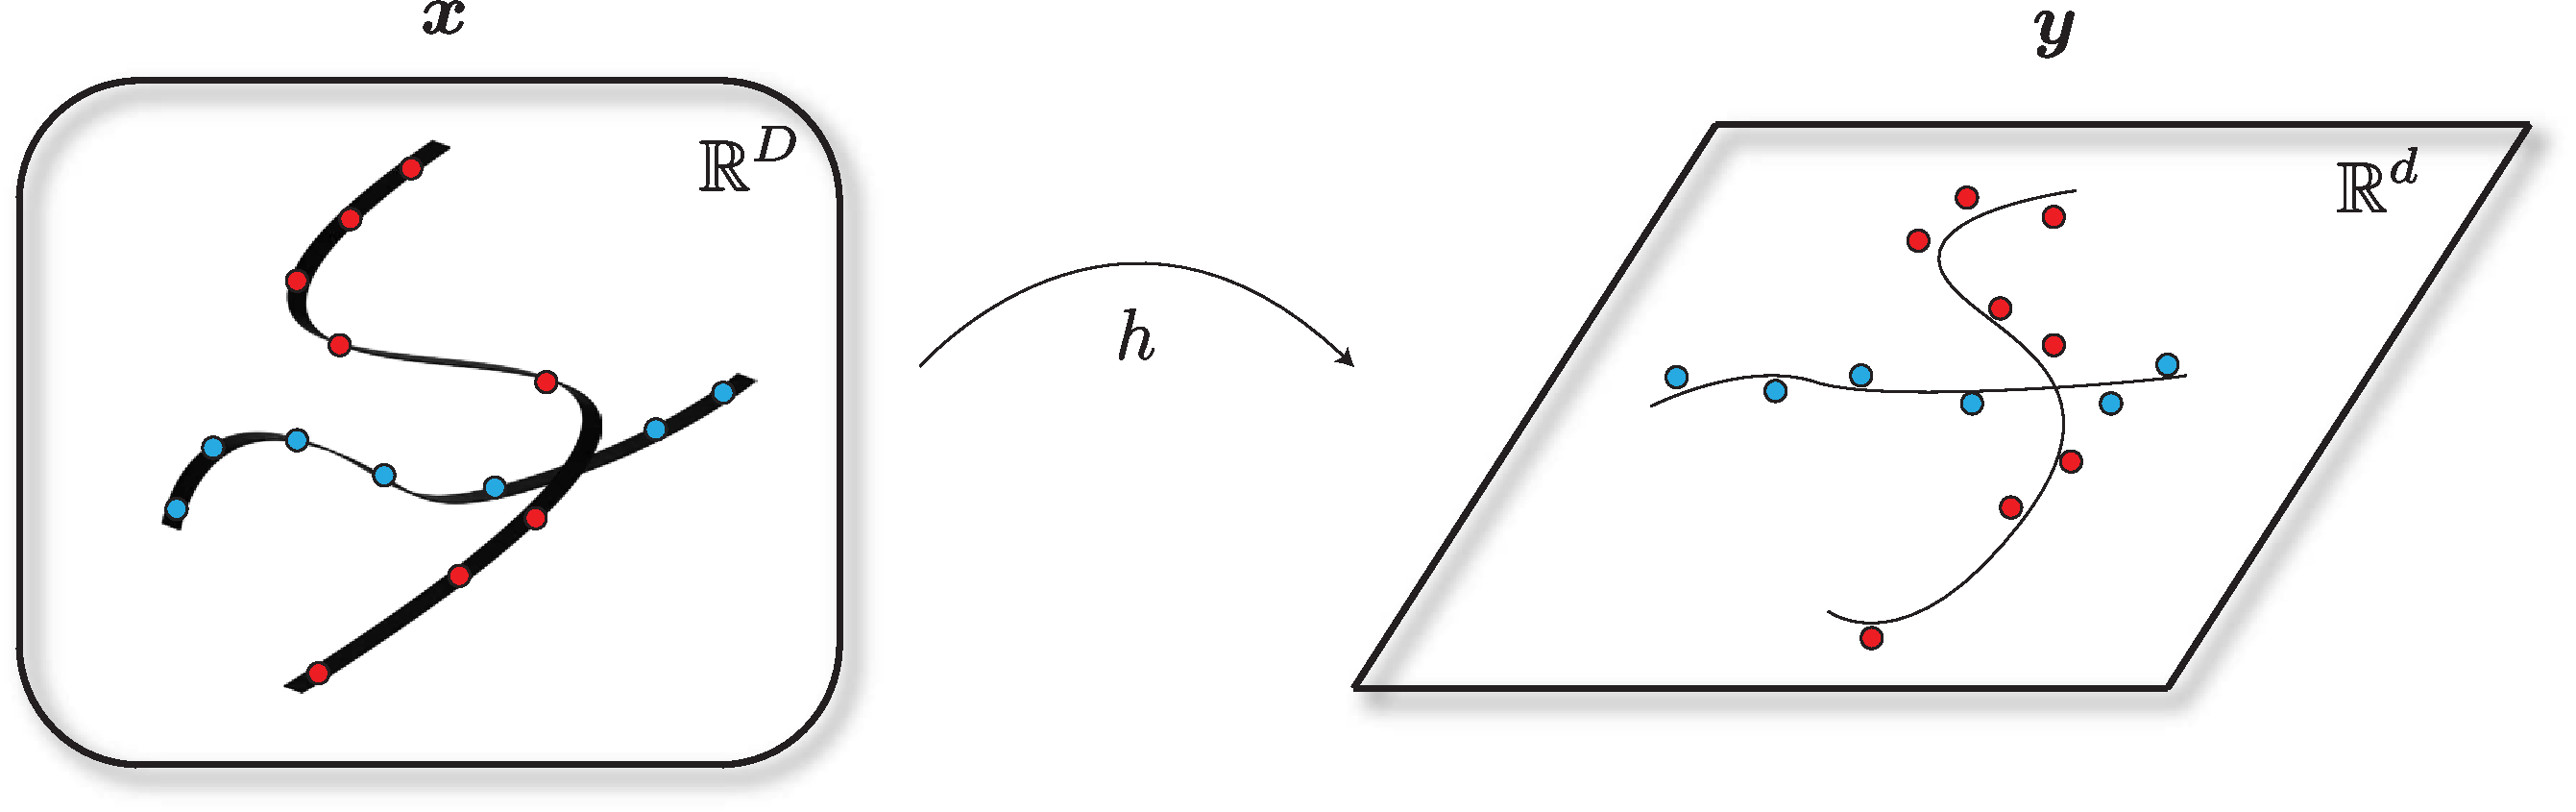
\includegraphics[width=0.9\textwidth]{\toplevelprefix/chapters/chapter6/figs/inference_roadmap.pdf}
  \caption{\small \textbf{Inferență cu distribuții de dimensiune redusă.} Aceasta este imaginea generică pentru acest capitol: avem o distribuție de dimensiune redusă pentru \(\vx \in \R^{D}\) (aici descrisă ca o uniune de două varietăți \(2\)-dimensionale în \(\R^{3}\)) și un model de măsurare \(\y = h(\vx) + \vw \in \R^{d}\). Vrem să inferăm diverse lucruri despre acest model, inclusiv distribuția condiționată a \(\vx\) dată \(\vy\), sau așteptarea condiționată \(\mathbb{E}[\vx \mid \y]\), date fiind diverse informații despre model și (potențial finite) eșantioane fie ale \(\vx\) fie ale \(\vy\).}
  \label{fig:inference_roadmap}
\end{figure}

\begin{example}[Completarea Imaginilor și Predicția Textului]
Completarea populară a imaginilor naturale și predicția limbajului natural sunt două sarcini tipice care ne cer să recuperăm date complete $\x$ din observațiile sale parțiale $\y$, cu părți din $\x$ mascate și de completat pe baza restului. Figura \ref{fig:image-text-completion} arată câteva exemple de astfel de sarcini. De fapt, sunt exact aceste sarcini care au inspirat cum să antrenăm modele mari moderne pentru generarea de text (cum ar fi GPT) și completarea imaginilor (cum ar fi autocodorul mascat) pe care le vom studia mai detaliat mai târziu.
    \begin{figure}
        \centering
        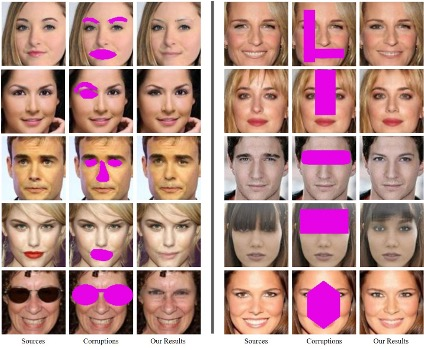
\includegraphics[height=0.4\linewidth]{\toplevelprefix/chapters/chapter6/figs/image-completion.jpg} \hspace{10mm} 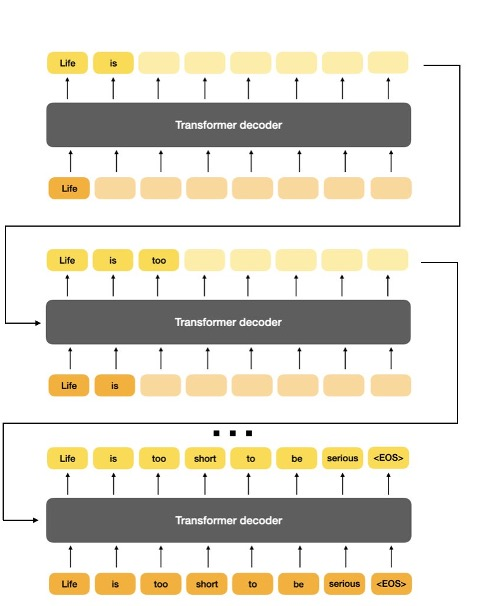
\includegraphics[height=0.45\linewidth]{\toplevelprefix/chapters/chapter6/figs/text-prediction.jpg}
        \caption{Stânga: completarea imaginii. Dreapta: predicția textului. În special, predicția textului este inspirația pentru popularul Transformer Generativ Pre-antrenat (GPT).}
        \label{fig:image-text-completion}
    \end{figure}
\end{example}


\paragraph{Interpretare statistică prin regula lui Bayes.} În general, pentru a îndeplini astfel de sarcini bine, trebuie să obținem distribuția condiționată $p(\x\mid \y)$. Dacă am avea aceasta, atunci am putea găsi estimarea de verosimilitate maximă (predicția): 
\begin{equation}
  \hat{\x} = \argmax_{\x} p(\x\mid \y);
\end{equation}
calcula estimarea așteptării condiționate: 
\begin{equation}
  \hat{\x} = \mathbb{E}[\x \mid \y] = \int \x p(\x\mid \y)\odif{\vx};
\end{equation}
și eșantiona din distribuția condiționată:  
\begin{equation}
  \hat{\x} \sim p(\x \mid \y).
\end{equation}

Observați că din regula lui Bayes, avem
\begin{equation}
  p(\x\mid \y) = \frac{p(\y\mid \x) p(\x) }{p(\y)}.
\end{equation} 
De exemplu, estimarea de verosimilitate maximă poate fi calculată rezolvând următorul program (log verosimilitate maximă):
\begin{equation}
    \hat{\x} = \argmax_{\x} [\log p(\y\mid \x) + \log p(\x)], 
\end{equation}
să zicem prin ascensiune gradient:
\begin{equation}
    \x_{k+1} = \x_k + \alpha \cdot \big(\nabla_{\x} \log p(\y \mid \x) + \nabla_{\x} \log p(\x)\big).
    \label{eqn:loglikelihoo-gradient-ascent}
\end{equation}
Calcularea eficientă a distribuției condiționate $p(\x \mid \y)$ depinde în mod natural de modul în care învățăm și exploatăm distribuția de dimensiune redusă $p(\x)$ a datelor $\x$ și modelul de observație $\y = h(\x) + \vw$ care determină distribuția condiționată $p(\y \mid \x)$.

\begin{remark}[Abordare End-to-End versus Bayesiană]
În practica modernă a învățării automate bazate pe date, pentru anumite sarcini populare oamenii adesea învață direct distribuția condiționată $p(\x\mid \y)$ sau o mapare (probabilistică) sau un regresor. O astfel de mapare este adesea modelată de unele rețele profunde și antrenată end-to-end cu suficiente eșantioane pereche $(\x, \y)$. O astfel de abordare este foarte diferită de abordarea bayesiană de mai sus în care sunt necesare atât distribuția lui $\x \sim p(\x)$, cât și maparea (de observație). Beneficiul abordării bayesiene este că distribuția învățată $p(\x)$ poate facilita multe sarcini diferite cu modele și condiții de observație variate.
\end{remark}

\paragraph{Interpretare geometrică ca optimizare constrânsă.}

Deoarece suportul \(\cS_{\vx}\) al distribuției lui \(\vx\) este de dimensiune redusă, putem presupune că există o funcție \(F\) astfel încât
\begin{equation}
  F(\vx) = \boldsymbol{0} \qquad \iff \qquad \vx \in \cS_{\vx}
\end{equation}
astfel încât \(\cS_{\vx} = F^{-1}(\{\vzero\})\) este suportul de dimensiune redusă al distribuției $p(\x)$. Geometric, o alegere naturală a lui $F(\x)$ este „funcția distanță" până la suportul $\mathcal{S}_{\x}$:\footnote{Observați că, în realitate, avem doar eșantioane discrete pe suportul distribuției. În același spirit de continuare, prin difuzie sau codare cu pierderi studiată în Capitolul \ref{ch:compression}, putem aproxima funcția distanță ca $F(\x) \approx \min_{\x_p \in \cC_{\vx}^{\epsilon}} \|\x - \x_p\|_2$ unde $\mathcal{S}_{\x}$ este înlocuit de o acoperire \(\cC_{\vx}^{\epsilon}\) a eșantioanelor cu bile de rază $\epsilon$.}
\begin{equation}
    F(\x) = \min_{\x_p \in \mathcal{S}_{\x}} \|\x - \x_p\|_2. 
\end{equation}
Acum, dat $\y = h(\x) +\vw$, pentru a rezolva pentru $\x$, putem rezolva următoarea problemă de optimizare constrânsă:
\begin{equation}
    \max_{\x} - \frac{1}{2}\|h(\x) - \y\|_2^2 \quad \mbox{s.t.} \quad F(\x) = \boldsymbol{0}. 
\end{equation}
Folosind metoda multiplicatorilor Lagrange augmentați, putem rezolva următorul program neconstrâns:
\begin{equation}
   \max_{\x} \left[-\frac{1}{2}\|h(\x) - \y\|_2^2  + \vlambda^{\top} F(\x) - \frac{\mu}{2} \|F(\x)\|_2^2\right]
\end{equation}
pentru anumiți multiplicatori Lagrange constanți $\vlambda$.
Aceasta este echivalentă cu următorul program:
\begin{equation}\label{eq:lagrange_multiplier_continuation}
\max_{\x} \left[\log \exp\Big(- \frac{1}{2}\|h(\x) - \y\|_2^2\Big) + \log \exp\Big( - \frac{\mu}{2} \big\|F(\x) - \vlambda/\mu\big\|_2^2\Big)\right],
\end{equation} 
unde $\vc \doteq {\vlambda}/{\mu}$ poate fi văzut ca o „medie" pentru funcția de constrângere. Pe măsură ce $\mu$ devine mare când se impune constrângerea prin continuare\footnote{În același spirit de continuare din \Cref{ch:compression} unde am obținut aproximări mai bune ale distribuției noastre trimițând \(\eps \to 0\), aici trimitem \(\mu \to \infty\). Valori mai mari ale lui \(\mu\) vor constrânge \(F\) să ia valori din ce în ce mai mici la optim, ceea ce înseamnă că optimul se află într-o vecinătate din ce în ce mai mică a suportului \(\cS_{\vx}\). Interesant, teoria multiplicatorilor Lagrange sugerează că, în anumite condiții benigne asupra \(F\) și altor termeni din obiectiv, trebuie doar să facem \(\mu\) suficient de mare pentru a asigura \(F(\vx) = \vzero\) la optim, ceea ce înseamnă că la o penalitate \textit{finită} obținem o aproximare \textit{perfectă} a suportului. În general, ar trebui să avem intuiția că \(\mu\) joacă același rol ca \(\epsilon^{-1}\).}, $\|\vc\|_2$ devine din ce în ce mai mic.

Programul de mai sus poate fi interpretat în două moduri diferite. În primul rând, se poate vedea primul termen ca probabilitatea condiționată a lui $\y$ dat $\x$, iar al doilea termen ca o densitate de probabilitate pentru $\x$:
\begin{equation}
  p(\y\mid \x) \propto \exp\Big(- \frac{1}{2}\|h(\x) - \y\|_2^2\Big), \quad 
    p(\x) \propto \exp\Big( - \frac{\mu}{2}\|F(\x) - \vc\|_2^2\Big).
\end{equation} 
Prin urmare, rezolvarea optimizării constrânse pentru problema inversă este echivalentă cu efectuarea inferenței Bayes cu densitățile de probabilitate de mai sus. Astfel, rezolvarea programului de mai sus \eqref{eq:lagrange_multiplier_continuation} prin ascensiune gradient este echivalentă cu estimarea de verosimilitate maximă de mai sus \eqref{eqn:loglikelihoo-gradient-ascent}, 
în care gradientul ia forma:
\begin{equation}
   \nabla_{\x} \log p(\y \mid \x) + \nabla_{\x} \log p(\x)   =  \pdv{h}{\vx}(\vx)\big(\y - h(\x)\big) + \mu \pdv{F}{\vx}(\vx)\big(\vc - F(\x)\big),
\end{equation}
unde $\pdv{h}{\vx}(\vx)$ și $\pdv{F}{\vx}(\vx)$ sunt Jacobianele lui $h(\x)$ și $F(\x)$, respectiv.

În al doilea rând, observați că programul de mai sus \eqref{eq:lagrange_multiplier_continuation} este echivalent cu:
\begin{equation}
\min_{\x} \frac{1}{2}\|h(\x) - \y\|_2^2 + \frac{\mu}{2} \big\|F(\x) - \vlambda/\mu\big\|_2^2,
\label{eqn:energy-minimization}
\end{equation} 
Datorită formei pătratice evidente a celor doi termeni, aceștia pot fi interpretați și ca anumite funcții de „energie". O astfel de formulare este adesea denumită „Minimizarea Energiei" în literatura de învățare automată.



\paragraph{Câteva setări practice reprezentative pentru inferență.} 
În practică, totuși, informațiile inițiale despre distribuțiile lui $\x$ și relația dintre $\x$ și $\y$ pot fi date în multe moduri și forme diferite. În general, ele pot fi în mare parte categorizate în patru cazuri, care sunt, conceptual, din ce în ce mai provocatoare:
\begin{itemize}
\item {\em Cazul 1:} Sunt cunoscute atât un model pentru distribuția lui $\x$, cât și modelul de observație $\y = h(\x)$ $(+ \boldsymbol{w})$, chiar cu o formă analitică. Acesta este de obicei cazul pentru multe probleme clasice de procesare a semnalului, cum ar fi eliminarea zgomotului din semnal, problema de recuperare a vectorului rar pe care l-am văzut în Capitolul \ref{ch:classic} și problema de recuperare a matricei de rang redus care va fi introdusă mai jos.
\item {\em Cazul 2:} Nu avem un model pentru distribuție, ci doar eșantioane $\X = \{\x_1, \ldots, \x_N\}$ ale lui $\x$, iar modelul de observație $\y = h(\x)$ $ (+ \boldsymbol{w})$ este cunoscut.\footnote{În literatură, această setare este uneori denumită {\em inferență bayesiană empirică}.} Un model pentru distribuția $p(\x)$ a lui $\x$ trebuie să fie învățat, iar ulterior distribuția condiționată $p(\x\mid \y)$. Completarea imaginilor naturale sau completarea limbajului natural (de exemplu, BERT și GPT) sunt exemple tipice ale acestei clase de probleme.
\item {\em Cazul 3:} Avem doar eșantioanele pereche: $(\X, \Y) = \{ (\x_1, \y_1), \ldots, (\x_N, \y_N) \}$ ale celor două variabile $(\x, \y)$. Distribuțiile lui $\x$ și $\y$ și relația lor $h(\cdot)$ trebuie să fie învățate din aceste date de eșantioane pereche. De exemplu, date fiind multe imagini și legendele lor, învățarea de a efectua generarea de imagini condiționată de text este o astfel de problemă.
\item {\em Cazul 4:} Avem doar eșantioanele $\Y = \{\y_1, \ldots, \y_N\}$ ale observațiilor $\y$, iar modelul de observație $h(\cdot)$ trebuie să fie cunoscut, cel puțin într-o familie parametrică $h(\cdot, \boldsymbol{\theta})$. Distribuția $p(\x)$ și $p(\x \mid \y)$ trebuie să fie învățate din $\hat \x$, estimate din $\Y$. De exemplu, învățarea de a reda o vizualizare nouă dintr-o secvență de vizualizări calibrate sau necalibrate este o astfel de problemă.
\end{itemize}
În acest capitol, vom discuta abordări generale pentru a învăța distribuțiile dorite și a rezolva estimarea condiționată asociată sau generarea pentru aceste cazuri, de obicei cu o problemă reprezentativă. Pe parcursul capitolului, ar trebui să păstrați în minte \Cref{fig:inference_roadmap}.





\section{Inferență Condiționată cu o Distribuție de Date Cunoscută}
Observați că în setarea pe care am discutat-o în capitolele anterioare, rețeaua de autocodare este antrenată să reconstruiască un set de eșantioane ale vectorului aleator $\x$. Acest lucru ne-ar permite să regenerăm eșantioane din distribuția (de dimensiune redusă) învățată. În practică, dimensionalitatea redusă a distribuției, odată dată sau învățată, poate fi exploatată pentru sarcini de recuperare, completare sau predicție stabile și robuste. Adică, în condiții destul de blânde, se poate recupera $\x$ din măsuri foarte compresive, parțiale, zgomotoase sau chiar corupte ale lui $\x$ de tipul:
\begin{equation}
    \y = h(\x) + \vw,
\end{equation}
unde $\y$ este de obicei o observație a lui $\x$ care este de dimensiune mult mai mică decât $\x$ și $\vw$ poate fi zgomot aleator sau chiar corupții brute rare. Aceasta este o clasă de probleme care au fost studiate pe larg în literatura clasică de procesare a semnalului, pentru structuri de dimensiune redusă cum ar fi vectori rari, matrici de rang redus și mai mult. Cititorii interesați pot vedea \cite{Wright-Ma-2022} pentru o expunere completă a acestui subiect.

Aici, pentru a pune lucrarea clasică într-un cadru modern mai general, ilustrăm ideea de bază și faptele prin sarcina, probabil cea mai simplă, de completare a datelor (și în special a imaginilor). Adică, considerăm problema de a recupera un eșantion $\x$ când părți din el lipsesc (sau chiar sunt corupte). Vrem să recuperăm sau să prezicem restul lui $\x$
din observarea doar a unei fracțiuni din el:
\begin{equation}
f: \mathcal{P}_{\Omega}(\x) \mapsto \hat{\x},
\end{equation}
unde $\mathcal{P}_{\Omega}(\spcdot)$ reprezintă o operație de mascare
(vezi \Cref{fig:matrix-completion} pentru un exemplu).

În această secțiune și următoarea, vom studia sarcina de completare în două scenarii diferite: Unul este când distribuția datelor $\x$ de interes este deja dată {\em apriori}, chiar într-o anumită formă analitică. Acesta este cazul care prevalează în procesarea clasică a semnalului unde structurile semnalelor sunt presupuse a fi cunoscute, de exemplu, cu bandă limitată, rare sau de rang redus. Celălalt este când sunt disponibile doar eșantioane brute ale lui $\x$ și trebuie să învățăm distribuția de dimensiune redusă din eșantioane pentru a rezolva bine sarcina de completare. Acesta este cazul pentru sarcinile de completare a imaginilor naturale sau predicție a cadrelor video. Ca un precursor al restului capitolului, începem cu cel mai simplu caz de completare a imaginii: când imaginea de completat poate fi bine modelată ca o matrice de rang redus. Vom trece la cazuri din ce în ce mai generale și setări mai provocatoare mai târziu.

\paragraph{Completarea matricei de rang redus.}  
Problema de {\em completare a matricei} de rang redus este o problemă clasică pentru completarea datelor când distribuția sa este de dimensiune redusă și cunoscută. Considerați un eșantion aleator al unei matrici $\X_o =
[\x_1, \ldots, \x_n] \in \mathbb{R}^{m\times n}$ din spațiul tuturor matricelor de rang $r$. În general, presupunem că rangul
matricei este
\begin{equation}
\mbox{rank}(\X_o) = r < \min\{m, n\}.
\end{equation}
Deci este clar că local dimensiunea intrinsecă a spațiului tuturor matricelor de rang $r$ este mult mai mică decât spațiul ambiental $mn$.

Acum, fie $\Omega$ să indice un set de indici ai intrărilor observate ale matricei $\X_o$. Fie intrările observate:
\begin{equation}
\Y = \mathcal{P}_{\Omega}(\X_o).
\end{equation}
Intrările rămase suportate pe $\Omega^c$ sunt neobservate sau
lipsă. Problema este dacă putem recupera din $\Y$ intrările lipsă
ale lui $\X$ corect și eficient. Figura \ref{fig:matrix-completion} arată un
exemplu de completare a unei astfel de matrici.

\begin{figure}
\centering
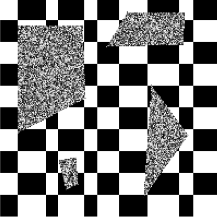
\includegraphics[width=0.3\linewidth]{\toplevelprefix/chapters/chapter6/figs/masked-checkerboard.png}\;\;

\includegraphics[width=0.3\linewidth]{\toplevelprefix/chapters/chapter6/figs/mask.png}\;\;
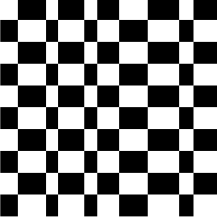
\includegraphics[width=0.3\linewidth]{\toplevelprefix/chapters/chapter6/figs/checkerboard.png}
\caption{Ilustrarea completării unei imagini ca matrice de rang redus
  cu unele intrări mascate sau corupte. Stânga: imaginea mascată/coruptă
$\Y$; mijloc: masca $\Omega$; dreapta: imaginea completată $\hat \X$.}
\label{fig:matrix-completion}
\end{figure}

Observați că motivul fundamental pentru care o astfel de matrice poate fi completată este că coloanele și rândurile matricei sunt foarte corelate și
toate se află pe un subspațiu de dimensiune redusă. Pentru exemplul arătat în
Figura \ref{fig:matrix-completion}, dimensiunea sau rangul matricei completate este doar doi. Prin urmare, ideea fundamentală pentru a recupera o astfel de matrice este să căutăm o matrice care are cel mai mic rang dintre toate
matricele care au intrări în acord cu cele observate:
\begin{equation}
\min_{\X} \mbox{rank}(\X) \quad \mbox{supus la}
\quad
\Y = \mathcal{P}_{\Omega}(\X).
\label{eqn:rank-min}
\end{equation}
Aceasta este cunoscută ca problema de {\em completare a matricei de rang redus}. Vezi \cite{Wright-Ma-2022} pentru o caracterizare completă a spațiului tuturor matricelor de rang redus. Deoarece funcția rang este discontinuă și minimizarea rangului
este în general o problemă NP-hard, am vrea să o relaxăm cu
ceva mai ușor de optimizat.

Bazându-ne pe cunoștințele noastre despre compresie din Capitolul
\ref{ch:compression}, am putea promova caracterul de rang redus al
matricei recuperate $\X$ impunând rata de codare cu pierderi (sau
volumul acoperit de $\X$) a datelor din $\X$ să fie mică:
\begin{equation}
\min R_\epsilon(\X) = \frac{1}{2} \log \det \left(\boldsymbol{I} +
\alpha  \X\X^\top \right) \quad \mbox{supus la}
\quad
\Y = \mathcal{P}_{\Omega}(\X).
\label{eqn:rate-min}
\end{equation}
Problema poate fi văzută ca o relaxare continuă a problemei de mai sus
de completare a matricei de rang redus \eqref{eqn:rank-min} și poate fi
rezolvată prin coborâre gradient. Se poate arăta că operatorul de coborâre gradient
pentru obiectivul $\log\det$ minimizează precis un
surogat apropiat al rangului matricei $\X\X^\top$.

Funcția de distorsiune a ratei este o funcție neconvexă, iar coborârea sa
gradient nu garantează întotdeauna găsirea soluției optime globale. Cu toate acestea, deoarece structura de bază căutată pentru $\X$ este liniară pe bucăți, funcția rang admite o relaxare convexă destul de eficace: norma
nucleară---suma tuturor valorilor singulare ale matricei $\X$. După
cum s-a arătat în literatura de detectare compresivă, în condiții destul de
largi,\footnote{De obicei, astfel de condiții specifică
cantitatea necesară și suficientă de intrări necesare pentru ca completarea
să fie fezabilă computațional. Aceste condiții au fost
caracterizate sistematic în \cite{Wright-Ma-2022}.} problema de
completare a matricei \eqref{eqn:rank-min}
poate fi rezolvată eficient prin următorul program convex:
\begin{equation}
\min \|\X\|_* \quad \mbox{supus la}
\quad
\Y = \mathcal{P}_{\Omega}(\X),
\label{eqn:nuclear-min}
\end{equation}
unde norma nucleară $\|\X\|_*$ este suma valorilor singulare ale
$\X$. În practică, adesea convertim programul de optimizare convex constrâns de mai sus
într-unul neconstrâns:
\begin{equation}
\min \|\X\|_*  + \lambda \|
\Y - \mathcal{P}_{\Omega}(\X)\|_F^2,
\label{eqn:nuclear-min-lagrangian}
\end{equation}
pentru un anumit $\lambda > 0$ ales corespunzător. Cititorii interesați pot consulta
\cite{Wright-Ma-2022} pentru cum să dezvolte algoritmi care pot rezolva
programele de mai sus eficient și eficace.
Figura \ref{fig:matrix-completion} arată un exemplu real în care
matricea $\hat \X$ este de fapt recuperată rezolvând programul de mai sus.

\paragraph{Extensii suplimentare.}
S-a arătat că imaginile (sau mai precis texturile) și scenele 3D
cu structuri de rang redus pot fi completate foarte eficient prin
rezolvarea programelor de optimizare de tipul de mai sus, chiar dacă există
corupție și distorsiune suplimentară
\cite{Zhang2010TILTTI,Liang-ECCV2012,Yi_2023_ICCV}:
\begin{equation}
    \Y \circ \tau = \X_o + \boldsymbol{E},
\end{equation}
unde $\tau$ este o distorsiune neliniară necunoscută a imaginii și $\boldsymbol{E}$ este o matrice necunoscută care modelează unele ocluziuni și corupții (rare). Din nou, cititorii interesați pot consulta \cite{Wright-Ma-2022} pentru o prezentare mai detaliată.

\section{Inferență Condiționată cu o Reprezentare de Date Învățată}
În subsecțiunea anterioară, motivul pentru care putem infera $\x$ din observația parțială $\y$ este pentru că (suportul) distribuției lui $\X$ este cunoscut sau specificat {\em apriori}, să zicem ca mulțimea tuturor matricelor de rang redus. Pentru multe seturi de date practice, nu avem distribuția lor într-o formă analitică precum matricele de rang redus, să zicem mulțimea tuturor imaginilor naturale. Cu toate acestea, dacă avem suficiente eșantioane ale datelor $\x$, ar trebui să putem învăța mai întâi distribuția sa de dimensiune redusă și să o valorificăm pentru sarcini viitoare de inferență bazate pe o observație $\y = h(\x) + \vw$. În această secțiune, presupunem că modelul de observație $h(\cdot)$ este dat și cunoscut. Vom studia cazul când $h(\cdot)$ nu este dat explicit în secțiunea următoare.


\subsection{Completarea Imaginilor cu Auto-Codare Mascată}
Pentru o imagine generală $\vX$ precum cea prezentată în stânga Figurii
\ref{fig:crate_mae_pipeline}, nu o mai putem vedea ca o matrice de rang
redus. Cu toate acestea, oamenii încă demonstrează o abilitate remarcabilă de a
completa o scenă și de a recunoaște obiecte familiare în ciuda ocluziunii
severe. Acest lucru sugerează că creierul nostru a învățat
distribuția de dimensiune redusă a imaginilor naturale și o poate folosi pentru
completare și, prin urmare, recunoaștere. Cu toate acestea, distribuția tuturor
imaginilor naturale nu este la fel de simplă ca un subspațiu liniar de dimensiune redusă.
Prin urmare, o întrebare naturală este dacă putem învăța distribuția mai
sofisticată a imaginilor naturale și o putem folosi pentru a efectua
completarea imaginilor?

\begin{figure}[t!]
\begin{center}
  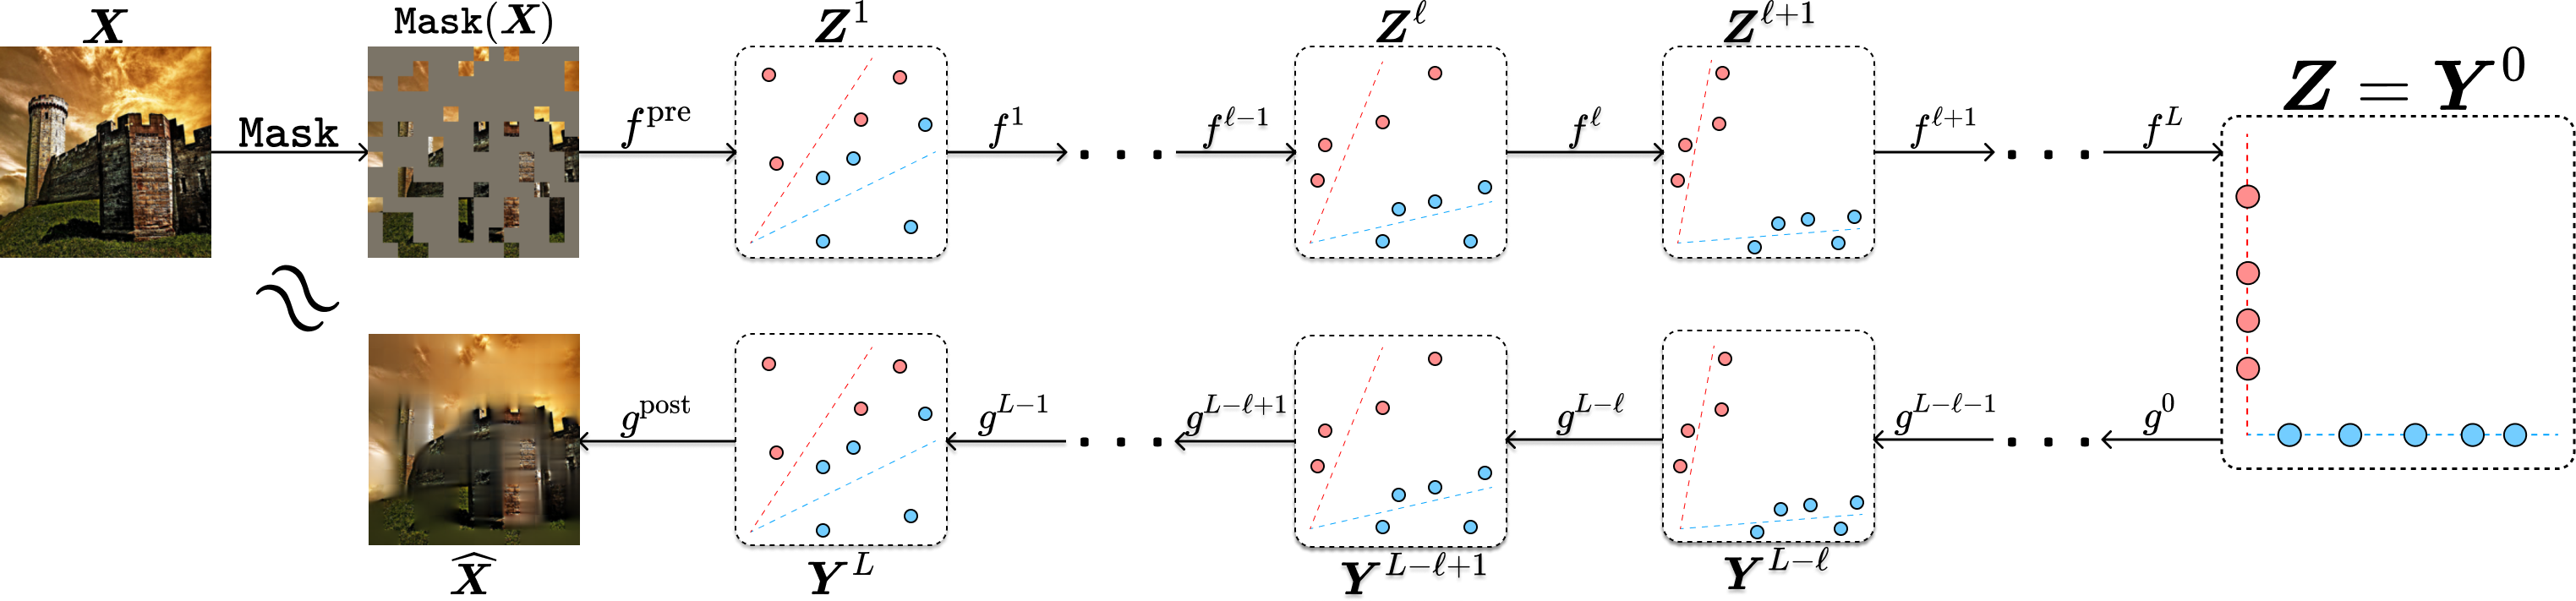
\includegraphics[width=0.99\textwidth]{\toplevelprefix/chapters/chapter6/figs/crate_mae_pipeline.png}
\end{center}
\caption{\small \textbf{Diagrama procesului general de autocodare (mascată).} Reprezentările token (imagine) sunt
  transformate iterativ către o reprezentare parsimonioasă (de exemplu, comprimată
  și rară) de fiecare strat codificator \(f^{\ell}\).
  Mai mult, astfel de reprezentări sunt transformate înapoi la
  imaginea originală de straturile decodificatorului \(g^{\ell}\). Fiecare strat codificator
  \(f^{\ell}\) este menit să fie (parțial) inversat de un
strat decodificator corespunzător \(g^{L - \ell}\).}
\label{fig:crate_mae_pipeline}
\end{figure}

O abordare empirică a sarcinii de completare a imaginii este să găsim o schemă de codare și decodare prin
rezolvarea următorului program de {\em autocodare mascată} (MAE) care
minimizează pierderea de reconstrucție:
\begin{equation}\label{eq:mae_loss}
\min_{f, g} L_{\mathrm{MAE}}(f, g) \doteq \mathbb{E}\big[\norm{(g \circ
f)(\mathcal{P}_\Omega(\vX)) - \vX}_{2}^{2}].
\end{equation}
Spre deosebire de problema de completare a matricei care are o structură
de bază simplă, nu ar trebui să ne mai așteptăm ca mapările de codare și decodare
să admită forme închise simple sau ca programul să poată fi rezolvat prin
algoritmi expliciți.

Pentru o imagine naturală generală, nu mai putem presupune că coloanele sau
rândurile sale sunt eșantionate dintr-un subspațiu de dimensiune redusă sau o
gaussiană de rang redus. Cu toate acestea, este rezonabil să presupunem că imaginea constă
din mai multe regiuni. Petele de imagine din fiecare regiune sunt similare și pot
fi modelate ca o gaussiană (de rang redus) sau un subspațiu. Prin urmare, pentru a exploata
dimensionalitatea redusă a distribuției, obiectivul \textit{codificatorului}
$f$ este să transforme $\X$ într-o reprezentare $\Z$:
\begin{equation}
    f: \X \mapsto \Z
\end{equation}
astfel încât distribuția lui $\Z$ să poată fi bine modelată ca un amestec de subspații, să zicem $\{\vU_{[K]}\}$,
astfel încât reducerea ratei să fie maximizată în timp ce raritatea este minimizată:
\begin{equation}\label{eq:sparse_rr}
\mathbb{E}_{\vZ = f(\vX)}[\Delta R_{\epsilon}(\vZ \mid \vU_{[K]}) - \lambda
\norm{\vZ}_{0}] = \mathbb{E}_{\vZ = f(\vX)}[R_\epsilon(\vZ) - R^{c}_\epsilon(\vZ \mid
\vU_{[K]}) - \lambda \norm{\vZ}_{0}],
\end{equation}
unde funcțiile $R_\epsilon(\cdot)$ și $R^c_\epsilon(\cdot)$ sunt definite în \eqref{eq:coding_rate} și \eqref{eq:def-mcr-Rc}, respectiv.

După cum am arătat în Capitolul anterior \ref{ch:representation},
codificatorul $f$ care minimizează obiectivul de mai sus poate fi construit ca
o secvență de operatori de tip transformer. După cum se arată în lucrarea lui
\cite{Pai2024masked}, decodificatorul $g$ poate fi văzut și, prin urmare,
construit explicit ca procesul invers al codificatorului $f$.
Figura \ref{fig:crate_mae_layers} ilustrează arhitecturile generale
atât ale codificatorului, cât și ale decodificatorului corespunzător la
fiecare strat. Parametrii codificatorului $f$ și decodificatorului $g$ pot fi
învățați optimizând pierderea de reconstrucție \eqref{eq:mae_loss} prin
coborâre gradient.

\begin{figure}[t!]
\centering
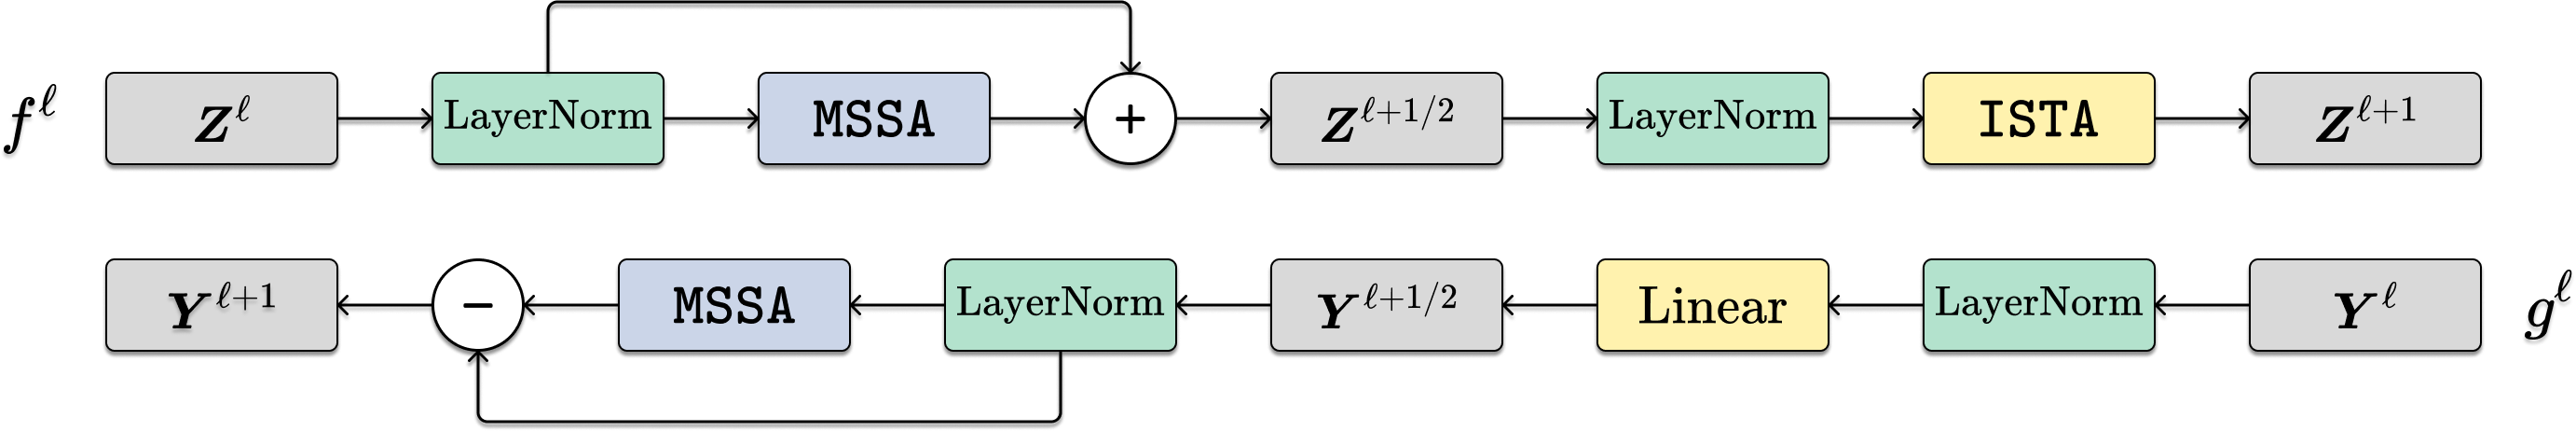
\includegraphics[width=0.99\textwidth]{\toplevelprefix/chapters/chapter6/figs/crate_mae_layers.png}
\caption{\small \textbf{Diagrama fiecărui strat codificator
  (\textit{sus}) și strat decodificator (\textit{jos}).} Observați că
  cele două straturi sunt foarte anti-paralele --- fiecare este construit să
  facă operațiile celuilalt în ordine inversă. Adică, în
  stratul decodificator \(g^{\ell}\), blocul \(\ISTA\) al \(f^{L - \ell}\)
  este parțial inversat mai întâi folosind un strat liniar, apoi
  blocul \(\MSSA\) al \(f^{L - \ell}\) este inversat; această ordine
desfășoară transformarea făcută în \(f^{L - \ell}\).}
\label{fig:crate_mae_layers}
\end{figure}

Figura \ref{fig:mae_autoencoding-small} arată câteva rezultate reprezentative
ale auto-codificatorului mascat astfel proiectat. Mai multe detalii de implementare și
rezultate ale autocodificatorului mascat pentru completarea imaginilor naturale pot fi
găsite în Capitolul \ref{ch:applications}.
\begin{figure}[t]
\centering
\includegraphics[width=0.99\textwidth]{\toplevelprefix/chapters/chapter6/figs/crate_mae_autoencoding_small.pdf}
\caption{\small \textbf{Vizualizări de autocodare ale CRATE-Base
  și ViT-MAE-Base \cite{he2022masked} cu 75\% din petele mascate.}
  Observăm că reconstrucțiile din CRATE-Base sunt la același nivel
  cu reconstrucțiile din ViT-MAE-Base, în ciuda utilizării \(<
  1/3\) din parametri.
}
\label{fig:mae_autoencoding-small}
\end{figure}




\subsection{Eșantionare Condiționată cu Potrivirea Măsurătorilor}
\label{sec:conditioned-decoding}
Problema de autocodare (mascată) de mai sus își propune să genereze o imagine eșantion care este consistentă cu anumite observații sau condiții. Dar să examinăm abordarea mai îndeaproape: dată
partea vizuală a unei imagini $\X_v = \mathcal{P}_{\Omega}(\X)$, încercăm să
estimăm partea mascată $\X_m = \mathcal{P}_{\Omega^c}(\X)$. Pentru realizările
$(\vXi_v, \vXi_m)$ ale variabilei aleatorii $\vX=(\vX_v, \vX_m)$, fie
\[p_{\X_m \mid \X_v}(\vXi_m\mid \vXi_v)\]
distribuția condiționată a $\X_m$ dată
$\X_v$. Este ușor de arătat că soluția optimă pentru formularea MAE
\eqref{eq:mae_loss} este dată de așteptarea condiționată:
\begin{equation}
  \argmin_{h = g \circ f}\, L_{\mathrm{MAE}}(h)
  = \vXi_v \mapsto \vXi_v + \mathbb{E}[\X_m \mid \X_v=\vXi_v].
\end{equation}
În general, totuși, această așteptare poate să nu se afle nici măcar pe
distribuția de dimensiune redusă a imaginilor naturale! Aceasta explică parțial
de ce unele dintre patch-urile recuperate în \Cref{fig:mae_autoencoding-small}
sunt puțin neclare.

Pentru multe scopuri practice, am dori să învățăm (o reprezentare
a) distribuției condiționate $p_{\X_m \mid \X_v}$, sau echivalent
$p_{\X \mid \X_v}$,
și apoi să obținem un eșantion clar (cel mai probabil) din această distribuție direct. Observați că, atunci când distribuția lui $\X$ este de dimensiune redusă, este posibil ca dacă o
parte suficientă din $\X$, $\X_v$, este observată, aceasta determină complet
$\X$ și prin urmare partea lipsă $\X_m$. Cu alte cuvinte, distribuția
$p_{\X \mid \X_v}$ este o funcție generalizată---dacă $\vX$ este complet determinat de $\vX_v$ aceasta este funcția delta, și mai general una dintre verii săi exotici.

Prin urmare, în loc să rezolvăm sarcina de completare ca o problemă de estimare condiționată, ar trebui să o abordăm ca o problemă de eșantionare condiționată. În acest scop, ar trebui mai întâi să învățăm distribuția (de dimensiune redusă) a tuturor imaginilor naturale $\X$. Dacă avem suficiente eșantioane de imagini naturale, putem învăța distribuția printr-un proces de eliminare a zgomotului $\X_t$ descris în Capitolul \ref{ch:compression}. Apoi problema de recuperare a $\X$ din observația sa parțială $\Y = \mathcal{P}_\Omega(\x) +\vw$ devine o problemă de generare condiționată -- de a eșantiona distribuția condiționată de observație.

\begin{figure}
  \centering
  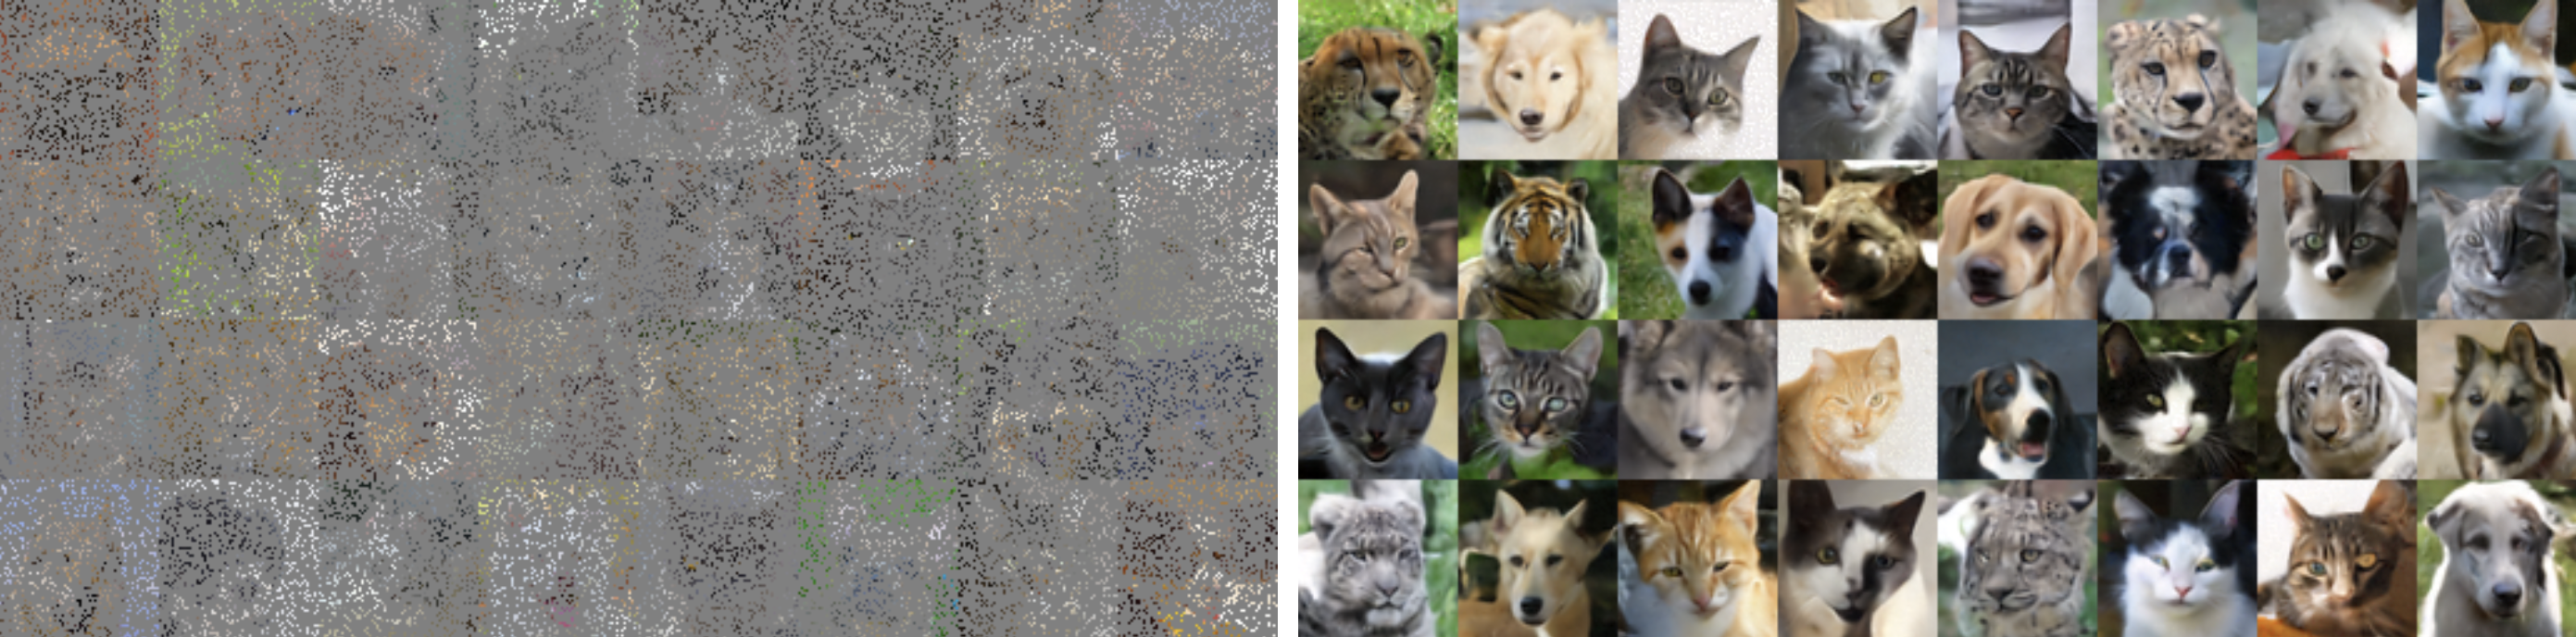
\includegraphics[width=1.0\textwidth]{\toplevelprefix/chapters/chapter6/figs/ambient_diffusion.png}
  \caption{\small \textbf{Vizualizări de eșantionare din modele antrenate prin difuzie ambientală \cite{Daras-NIPS2023} cu 80\% din pixeli mascați.} Folosind un raport similar de pixeli mascați ca în \Cref{fig:mae_autoencoding-small}, algoritmul de eșantionare prin difuzie ambientală recuperează o imagine mult mai clară decât imaginea neclară recuperată prin metoda bazată pe MAE. Prima metodă eșantionează din distribuția imaginilor naturale, în timp ce ultima aproximează așteptarea condiționată (adică media) acestei distribuții dată observația; această mediere cauzează neclaritatea.}
  \label{fig:ambient_diffusion}
\end{figure}

\paragraph{Măsurători liniare generale.} 
De fapt, putem considera chiar recuperarea lui $\X$ dintr-un model de observație liniară mai general:
\begin{equation}
    \Y = \vA\X_0,  \quad \X_t = \X_0 + \sigma_t \vG,  
\end{equation}
unde $\vA$ este un operator liniar pe spațiul matricelor\footnote{adică, dacă ne imaginăm desfășurarea lui \(\vX\) într-un vector lung, atunci \(\vA\) ia rolul unei matrici pe spațiul \(\vX\)} și $\vG \sim \mathcal{N}(\boldsymbol{0}, \vI)$. Operatorul de mascare $\mathcal{P}_{\Omega}(\cdot)$ din sarcina de completare a imaginii este un exemplu de astfel de model liniar. Atunci s-a arătat de \cite{daras2023ambient} că 
\begin{equation}
    \hat{\X}_* = \argmin_{\hat{\X}} \mathbb{E}[\|\vA(\hat{\X}(\vA\X_t, \vA) - \X_0)\|^2]
\end{equation}
satisface condiția că:
\begin{equation}
    \vA \hat{\X}_*(\vA(\X_t), \vA) = \vA \mathbb{E}[\X_0 \mid \vA \X_t, \vA].
\end{equation} Observați că în cazul special când $\vA$ este de rang complet pe coloane, avem $ \mathbb{E}[\X_0 \mid \vA\X_t, \vA] = \mathbb{E}[\X_0 \mid \X_t]$. Prin urmare, în cazul mai general, s-a sugerat de \cite{daras2023ambient} că se poate încă folosi $\mathbb{E}[\X_0 \mid \vA(\X_t), \vA]$ astfel obținut pentru a înlocui $\mathbb{E}[\X_0 \mid \X_t]$ în procesul normal de eliminare a zgomotului pentru $\X_t$:
\begin{equation}
    \X_{t-s} = \gamma_t \X_t + (1-\gamma_t) \mathbb{E}[\X_0 \mid \vA\X_t, \vA].
\end{equation}
Aceasta funcționează de obicei foarte bine în practică, să zicem pentru multe sarcini de restaurare a imaginilor, așa cum se arată în \cite{daras2023ambient}. În comparație cu imaginile neclare recuperate din MAE, imaginile recuperate prin metoda de mai sus sunt mult mai clare deoarece valorifică o distribuție învățată a imaginilor naturale și eșantionează o imagine (clară) din distribuția care este consistentă cu măsurarea, așa cum se arată în \Cref{fig:ambient_diffusion} (cf \Cref{fig:mae_autoencoding-small}).


\paragraph{Măsurători neliniare generale.}
Pentru a generaliza problemele de completare a (imaginilor) de mai sus și a face lucrurile mai riguroase, putem considera că un vector aleator $\vx \sim p$ este parțial observat printr-o funcție de observație mai
generală:
\begin{equation}\label{eq:measurement-matching-observation}
\vy = h(\vx) + \vw,
\end{equation}
unde $\vw$ reprezintă de obicei un anumit zgomot de măsurare aleator, să zicem de
o distribuție gaussiană $\vw \sim \mathcal{N}(\mathbf{0}, \sigma^2
\boldsymbol{I})$. Este ușor de văzut că, pentru $\x$ și $\y$ astfel legate, distribuția lor comună $p(\x, \y)$ este în mod natural aproape degenerată dacă zgomotul $\vw$ este mic. În mare măsură, putem vedea $p(\x, \y)$ ca o versiune zgomotoasă a unei hipersuprafețe definite de funcția $\y = h(\x)$ în spațiul comun $(\x, \y)$. Practic vorbind, vom considera o setare mai asemănătoare cu autocodarea mascată decât cu completarea pură a matricei, unde avem întotdeauna acces la un eșantion curat corespunzător $\vx$ pentru fiecare observație $\vy$ pe care o primim.\footnote{În unele aplicații mai specializate, în special în imagistica științifică, este de interes să putem învăța să generăm eșantioane din posteriorul $p_{\x \mid \y}$ fără acces la niciun eșantion curat/adevăr de bază al lui $\x$. Oferim o scurtă prezentare generală a metodelor pentru această setare în notele de final de capitol.}

La fel ca completarea imaginii/matricei, suntem
adesea confruntați cu o setare în care $\vy$ denotă o observație degradată sau altfel
„cu pierderi"
a intrării $\vx$. Aceasta se poate manifesta în forme destul de diferite.
De exemplu, în diverse probleme de imagistică științifică sau
medicală, datele măsurate $\vy$ pot fi o observație comprimată și
coruptă a datelor de bază $\vx$; în timp ce în sarcini de viziune 3D,
$\vy$ poate reprezenta o imagine capturată de o cameră a unui obiect fizic cu o
poză (de dimensiune redusă) necunoscută $\vx$.
În general, în virtutea modelării matematice (și, în unele cazuri, co-proiectării
sistemului de măsurare), cunoaștem $h$ și o putem evalua pe orice intrare, și
putem exploata aceste cunoștințe pentru a ajuta la reconstrucția și eșantionarea lui $\vx$.

\begin{figure}[t]
  \centering
  \begin{subfigure}{0.45\textwidth}
    \vspace{0.75cm}
    \centering
    \begin{tikzcd}[column sep=1.5cm]
      \vx \arrow[r, "h(\vx) + \vw"] & \vy \arrow[r, "p_{\vx \mid \vy}"]
      & \posteriorsample \arrow[r, "\posteriorsample + t\vg"] & \posteriorsample_t
    \end{tikzcd}
    \vspace{0.75cm}
    \caption{}
    \label{fig:left}
  \end{subfigure}
  \hfill
  \begin{subfigure}{0.45\textwidth}
    \centering
    \begin{tikzcd}[column sep=1.5cm, row sep=0.5cm]
    & \vy \\
    \vx \arrow[ur, "h(\vx) + \vw"] \arrow[dr, "\vx + t\vg"] & \\
    & \vx_t
    \end{tikzcd}
    \caption{}
    \label{fig:right}
  \end{subfigure}
  \caption{Diagrame de dependență statistică pentru procesul de eșantionare condiționată.
  \textbf{Stânga:} Într-o aplicație directă (conceptuală) a schemei de difuzie-eliminare a zgomotului
  pe care am dezvoltat-o în \Cref{ch:compression} pentru eșantionarea condiționată, folosim
  eșantioane din posteriorul $p_{\vx \mid \vy}$ pentru a antrena eliminatoare de zgomot direct pe
  posterior la diferite niveluri de zgomot, apoi le folosim pentru a genera noi
  eșantioane. În practică, totuși, nu avem în mod normal eșantioane directe din
  posterior, ci mai degrabă eșantioane pereche $(\vx, \vy)$ din distribuția comună.
  \textbf{Dreapta:} Se dovedește că este suficient să avem doar observații zgomotoase
  ale lui $\vx$ pentru a realiza eliminatoarele de zgomot corespunzătoare lui $p_{\posteriorsample_t \mid
  \posteriorsample}$: aceasta rezultă din independența condiționată a lui $\vx_t$ și
  $\vy$ dat $\vx$. Aceasta implică că $p_{\posteriorsample_t} = p_{\vx_t \mid
  \vy}$, ceea ce dă o funcție de scor pentru eliminarea zgomotului care constă din
  funcția de scor necondiționată, plus un termen de corecție care impune
  consistența măsurătorii.}
  \label{fig:posterior-sampling-cds}
\end{figure}


La nivel tehnic, vrem ca reprezentarea învățată a datelor
să ne faciliteze eșantionarea distribuției condiționate $p_{\vx\mid
\vy}$, cunoscută și ca posterior, eficace și eficient. Mai precis,
scriem $\vnu$ pentru a denota o realizare a variabilei aleatorii $\vy$.
Vrem să generăm eșantioane $\hat{\x}$ astfel încât:
\begin{equation}\label{eq:goal-sample-posterior}
  \hat{\x} \sim   p_{\vx \mid \y}(\spcdot \mid \vy=\vnu).
\end{equation}

Reamintim că în \Cref{sub:compression_denoising}, am dezvoltat un mod natural și
eficace de a produce eșantioane \textit{necondiționate} ale distribuției datelor
$p$. Ingredientele sunt denoiser-ele $\bar{\x}^\ast(t, \vxi) = \bE[ \x \mid
\vx_t=\vxi ]$, sau aproximările lor învățate $\bar{\x}_{\theta}(t, \vxi)$,
pentru diferite niveluri de observații zgomotoase $\x_t = \x + t \vg$ (și $\vxi$ pentru
realizările lor) sub
zgomot Gaussian $\vg \sim \cN(\mathbf{0}, \vI)$, și $t \in
[0, T]$ cu o alegere de timpi $0 = t_1 < \hdots < t_{L} = T$ la care să
efectuăm denoising-ul iterativ, începând de la $\hat{\vx}_{t_L} \sim
\cN(\mathbf{0}, T^2 \vI)$ (reamintiți \Cref{eq:denoising-iteration-basic}).\footnote{Reamintim din discuția noastră în \Cref{sub:sampling_denoising}
că câteva îmbunătățiri mici la această schemă de denoising iterativ de bază sunt
suficiente pentru a aduce performanță practică competitivă. Pentru claritate pe măsură ce dezvoltăm
eșantionarea condiționată, ne vom concentra aici pe cea mai simplă instanțiere.}
Am putea aplica direct această schemă pentru a genera eșantioane din posteriorul
$p_{\vx \mid \vy}$ \textit{dacă} am avea acces la un set de date de eșantioane
$\posteriorsample \sim p_{\vx \mid \y}(\spcdot \mid \vnu)$ pentru fiecare realizare
$\vnu$ a $\vy$, prin generarea de observații zgomotoase
$\posteriorsample_t$ și antrenarea de denoiser-e pentru a aproxima $\bE[
  \posteriorsample \mid \posteriorsample_t=\spcdot, \vy=\vnu ]$, media posteriorului sub
observația zgomotoasă (vezi \Cref{fig:posterior-sampling-cds}(a)).
Totuși, efectuarea acestei re-eșantionări având doar eșantioane pereche $(\vx, \vy)$ din distribuția
comună (să zicem prin gruparea eșantioanelor pe valori ale $\vy$) necesită
prohibitiv de multe eșantioane pentru date de dimensiune înaltă, iar abordările alternative
se bazează explicit sau implicit pe estimarea densității, care suferă în mod similar de
blestemul dimensionalității.

Din fericire, se dovedește că acest lucru nu este necesar.
Considerați diagrama alternativă de dependență statistică din
\Cref{fig:posterior-sampling-cds}(b), care corespunde variabilelor aleatoare
din procesul obișnuit de denoising-difuzie, împreună cu măsurătoarea $\vy$. 
Deoarece modelul nostru de observație presupus \eqref{eq:measurement-matching-observation}
implică că $\vx_t$ și $\vy$ sunt independente condiționate de $\vx$, avem pentru
orice realizare $\vnu$ a $\vy$
\begin{equation}\label{eq:conditional-denoising-conditioning-order-irrelevant}
  \begin{split}
  p_{\posteriorsample_t\mid \vy}(\spcdot \mid \vnu)
  &= \int
  \underbrace{p_{\posteriorsample_t \mid \posteriorsample}(\spcdot\mid \vxi)}_{=
  \cN(\vxi, t^2 \vI)}
  \spcdot \underbrace{p_{\posteriorsample \mid \vy}}_{= p_{\vx\mid \vy}}(\vxi \mid
  \vnu)
  \odif \vxi
  \\
  &=
  \int p_{\vx_t \mid \vx, \vy}(\spcdot\mid \vxi, \vnu) \spcdot p_{\vx \mid
  \vy}(\vxi\mid \vnu) \odif \vxi
  \\
  &=
  \int p_{\vx_t, \vx \mid \vy}(\spcdot, \vxi \mid \vnu) \odif \vxi
  \\
  &= p_{\vx_t \mid \vy}(\spcdot\mid \vnu).
  \end{split}
\end{equation}
Mai sus, prima linie recunoaște o echivalență între distribuțiile
care apar în \Cref{fig:posterior-sampling-cds} (a,b); a doua linie aplică aceasta
împreună cu independența condiționată a $\vx_t$ și $\vy$ date $\vx$; a
treia linie folosește definiția probabilității condiționate; iar linia finală
marginalizează peste $\vx$.
Astfel, denoiser-ele din procesul conceptual de eșantionare posterioară sunt egale cu
$\bE[\vx \mid \vx_t=\spcdot, \vy=\vnu]$, pe care le putem învăța doar din eșantioane pereche $(\vx,
\vy)$,
și prin formula lui Tweedie (\Cref{thm:tweedie}), putem exprima aceste denoiser-e în
termenii funcției scor a $p_{\vx_t \mid \vy}$, care, prin regula lui Bayes,
satisface
\begin{equation}
  p_{\vx_t \mid \vy}(\vxi \mid \vnu) 
  = \frac{p_{\vy \mid \vx_t}(\vnu \mid \vxi) p_{\vx_t}(\vxi)}{p_{\vy}(\vnu)}.
\end{equation}
Reamintim că densitatea lui $\vx_t$ este 
dată de $p_t = \varphi_{t} \ast p$, unde $\varphi_{t}$ denotă
densitatea Gaussiană standard cu medie zero și covarianță $t^2 \vI$ iar $\ast$ denotă
convoluția. Aceasta nu este altceva decât \textit{funcția scor necondiționată}
obținută din antrenarea standard de difuzie pe care am dezvoltat-o în
\Cref{sub:compression_denoising}!
Funcția scor condiționată satisface atunci, pentru orice realizare $(\vxi,
\vnu)$ a $(\vx_t, \vy)$,
\begin{equation}
  \nabla_{\vxi} \log p_{\vx_t \mid \vy}(\vxi\mid \vnu)
  =
  \underbrace{\nabla_{\vxi} \log p_t(\vxi)}_{\text{potrivire scor}}
  +
  \underbrace{\nabla_{\vxi} \log p_{\vy \mid \vx_t}(\vnu \mid \vxi)}_{\text{potrivire măsurătoare}},
  \label{eqn:conditional-denoising-score}
\end{equation}
dând (prin formula lui Tweedie) denoiser-ele noastre propuse ca
\begin{align*}
  \bE[ \vx \mid \vx_t=\vxi, \vy=\vnu]
  &=
  \vxi + t^2 \nabla_{\vxi}\log p_t(\vxi) + t^2 \nabla_{\vxi}\log p_{\vy \mid
  \vx_t}(\vnu \mid \vxi)
  \\
  &=
  \bE[\vx \mid \vx_t=\vxi] + t^2 \nabla_{\vxi}\log p_{\vy \mid \vx_t}(\vnu\mid
  \vxi).
  \labelthis \label{eq:posterior-sampling-denoiser-decomposition}
\end{align*}
Operatorii rezultați sunt interpretabili ca o versiune \textit{corectată} a
denoiser-ului necondiționat pentru observația zgomotoasă, unde termenul de corecție (așa-numitul
termen de ``potrivire a măsurătorii'') impune consistența cu
observațiile $\vy$. Cititorul ar trebui să fie atent să observe la care argument se
aplică operatorii gradient în funcțiile scor de mai sus pentru a înțelege pe deplin
sensul acestui operator.

Problema cheie rămasă în a face această procedură computațională este să prescriem
cum să calculăm corecția de potrivire a măsurătorii, deoarece în general nu avem
o expresie în formă închisă
pentru verosimilitatea $p_{\vy \mid \vx_t}$ cu excepția cazului când $t
= 0$. Înainte de a aborda această problemă, discutăm un exemplu concret ilustrativ
al întregului proces, continuând de la cele pe care le-am dezvoltat în
\Cref{sub:compression_denoising}.

\begin{example}\label{example:denoising-conditional-gaussian}
  Considerați cazul în care distribuția datelor este Gaussiană cu media $\vmu \in
  \bR^D$ și
  covarianța $\vSigma \in \bR^{D \times D}$, adică $\vx \sim \cN(\vmu, \vSigma)$.
  Presupunem că $\vSigma \succeq \Zero$ este nenulă.
  Mai mult, în modelul de măsurare \eqref{eq:measurement-matching-observation},
  să presupunem că obținem măsurători liniare ale $\vx$ cu zgomot Gaussian
  independent, unde $\vA \in \bR^{d \times D}$ și $\vy = \vA \vx + \sigma \vw$
  cu $\vw \sim \cN(\Zero, \vI)$ independent de $\vx$.
  Atunci $\vx =_{d} \vSigma^{1/2} \vg + \vmu$, unde $\vg \sim \cN(\Zero, \vI)$ este
  independent de $\vw$ și $\vSigma^{1/2}$ este rădăcina pătrată pozitivă unică a
  matricei de covarianță $\vSigma$, și
  după câteva calcule algebrice, putem scrie apoi
  \begin{equation*}
    \begin{bmatrix}
      \vx \\
      \vy
    \end{bmatrix}
    =_{d}
    \begin{bmatrix}
      \vSigma^{1/2} & \Zero \\
      \vA \vSigma^{1/2} & \sigma \vI
    \end{bmatrix}
    \begin{bmatrix}
      \vg \\
      \vw
    \end{bmatrix}
    +
    \begin{bmatrix}
      \vmu \\
      \vA\vmu
    \end{bmatrix}.
  \end{equation*}
  Prin independență, avem că $(\vg, \vw)$ este Gaussian comun, ceea ce înseamnă că
  $(\vx, \vy)$ este de asemenea Gaussian comun, ca imagine afină a unui
  vector Gaussian comun.
  Matricea sa de covarianță este dată de
  \begin{equation*}
    \begin{bmatrix}
      \vSigma^{1/2} & \Zero \\
      \vA \vSigma^{1/2} & \sigma \vI
    \end{bmatrix}
    \begin{bmatrix}
      \vSigma^{1/2} & \Zero \\
      \vA \vSigma^{1/2} & \sigma \vI
    \end{bmatrix}^\top
    =
    \begin{bmatrix}
      \vSigma & \vSigma \vA^\top \\
      \vA \vSigma & \vA \vSigma \vA^\top + \sigma^2 \vI
    \end{bmatrix}.
  \end{equation*}
  Acum, aplicăm faptul că condiționarea unui vector aleator cu distribuție Gaussiană comună
  pe un subset de coordonate este din nou o distribuție Gaussiană
  (\Cref{exercise:conditional_gaussian}).
  Prin aceasta, obținem că
  \begin{equation}
    p_{\x \mid \y}(\spcdot \mid \vnu) = \cN\left(
    \underbrace{%
      \vmu + \vSigma\vA^\top \left(\vA\vSigma\vA^\top + \sigma^2 \vI\right)^{-1} 
      (\vnu - \vA\vmu)}_{\vmu_{\vx \mid \vy}(\vnu)},
      \underbrace{%
      \vSigma - \vSigma \vA^\top \left(\vA\vSigma\vA^\top + \sigma^2
      \vI\right)^{-1} \vA \vSigma}_{\vSigma_{\vx\mid \vy}}
    \right).
  \end{equation}
  Prin echivalența pe care am derivat-o mai sus, obținem printr-o altă aplicare a
  \Cref{exercise:conditional_gaussian}
  \begin{equation}\label{eq:conditional-posterior-denoiser-gaussian-case}
    \bE[ \vx \mid \vx_t=\vxi, \vy=\vnu ]
    =
    \vmu_{\vx\mid \vy}(\vnu) + \vSigma_{\vx\mid\vy}\left(
    \vSigma_{\vx\mid \vy} + t^2 \vI 
    \right)^{-1}\left(
    \vxi - \vmu_{\vx\mid \vy}(\vnu)
    \right).
  \end{equation}
  Forma funcțională a acestui denoiser este destul de simplă, dar poartă o
  dependență greoaie de datele problemei $\vmu$, $\vSigma$, $\vA$ și
  $\sigma^2$.
  Putem obține o înțelegere suplimentară a comportamentului său comparându-l cu
  \Cref{eq:posterior-sampling-denoiser-decomposition}.
  Avem ca de obicei
  \begin{equation}\label{eq:posterior-denoiser-gaussian-case}
    \bE[\vx \mid \vx_t=\vxi]
    = \vmu + \vSigma\left(\vSigma + t^2 \vI\right)^{-1} (\vxi - \vmu),
  \end{equation}
  care este destul de simplu---sugerând că termenul de potrivire a măsurătorii este
  destul de complicat. Pentru a confirma aceasta, putem calcula verosimilitatea $p_{\vy
  \mid \vx_t}$ direct folosind următoarea expresie pentru distribuția comună
  a $(\vx_t, \vy)$:
  \begin{equation}
    \begin{bmatrix}
      \vx \\
      \vx_t \\
      \vy
    \end{bmatrix}
    =_{d}
    \begin{bmatrix}
      \vSigma^{1/2} & \Zero & \Zero \\
      \vSigma^{1/2} & t\vI & \Zero \\
      \vA \vSigma^{1/2} & \Zero & \sigma \vI
    \end{bmatrix}
    \begin{bmatrix}
      \vg \\
      \vg' \\
      \vw
    \end{bmatrix}
    +
    \begin{bmatrix}
      \vmu \\
      \vmu \\
      \vA\vmu
    \end{bmatrix},
  \end{equation}
  unde $\vg' \sim \cN(\Zero, \vI)$ independent de celelalte Gaussiene.
  Aceasta este din nou o distribuție Gaussiană comună; restricționând doar la ultimele
  două rânduri, avem covarianța
  \begin{equation*}
    \begin{bmatrix}
      \vSigma^{1/2} & t\vI & \Zero \\
      \vA \vSigma^{1/2} & \Zero & \sigma \vI
    \end{bmatrix}
    \begin{bmatrix}
      \vSigma^{1/2} & t\vI & \Zero \\
      \vA \vSigma^{1/2} & \Zero & \sigma \vI
    \end{bmatrix}^\top
    =
    \begin{bmatrix}
      \vSigma + t^2\vI & \vSigma\vA^\top \\
      \vA\vSigma & \vA\vSigma\vA^\top + \sigma^2 \vI
    \end{bmatrix}.
  \end{equation*}
  O altă aplicare a \Cref{exercise:conditional_gaussian} ne dă apoi
  \begin{equation}
    p_{\y \mid \vx_t}(\spcdot \mid \vxi) = \cN\left(
    \underbrace{%
      \vA\vmu + \vA\vSigma\left( \vSigma + t^2 \vI \right)^{-1}
      \left(
        \vxi - \vmu
      \right)
      }_{\vmu_{\vy \mid \vx_t}(\vxi)},
      \underbrace{%
        \vA\vSigma\vA^\top + \sigma^2 \vI - \vA\vSigma \left( \vSigma
        + t^2 \vI\right)^{-1} \vSigma \vA^\top
      }_{\vSigma_{\vy\mid \vx_t}}
    \right).
  \end{equation}
  Acum observați că $\vmu_{\vy \mid \vx_t}(\vxi) = \vA \bE[\vx \mid \vx_t=\vxi]$.
  Deci, prin regula lanțului,
  \begin{align*}
    t^2 \nabla_{\vxi} \log p_{\vy \mid \vx_t}(\vnu \mid \vxi)
    &=
    t^2 \nabla_{\vxi}\left[
      -\frac{1}{2}
      (\vnu - \vA \bE[\vx \mid \vx_t=\vxi])^\top
      \vSigma_{\vy \mid \vx_t}^{-1}
      (\vnu - \vA \bE[\vx \mid \vx_t=\vxi])
      \right]
    \\
    &= t^2 (\vSigma+t^2 \vI)^{-1}\vSigma\vA^\top\vSigma_{\vy \mid \vx_t}^{-1}\left(
    \vnu - \vA \bE[\vx \mid \vx_t=\vxi] \right).
    \labelthis
    \label{eq:conditional-posterior-measurementmatching-gaussian-case}
  \end{align*}
  Aceasta ne dă o descompunere mai interpretabilă a denoiser-ului posterior condiționat
  \eqref{eq:conditional-posterior-denoiser-gaussian-case}: urmând
  \Cref{eq:posterior-sampling-denoiser-decomposition}, este suma denoiser-ului
  posterior necondiționat \eqref{eq:posterior-denoiser-gaussian-case}
  și termenul de potrivire a măsurătorii
  \eqref{eq:conditional-posterior-measurementmatching-gaussian-case}.
  Putem analiza în continuare termenul de potrivire a măsurătorii. Observați că
  \begin{equation}
    \vSigma_{\vy \mid \vx_t}
    =
    \sigma^2 \vI + \vA\vSigma^{1/2} \left(
      \vI - \vSigma^{1/2}\left(
      \vSigma + t^2 \vI
      \right)^{-1}
      \vSigma^{1/2}
    \right)\vSigma\vA^\top.
  \end{equation}
  Dacă notăm $\vSigma = \vV \vLambda \vV^\top$ o descompunere în valori proprii
  a $\vSigma$, unde $(\vv_i)$ sunt coloanele lui $\vV$, putem scrie mai departe
  \begin{align}
    \vSigma^{1/2}\left(
    \vI - \vSigma^{1/2}\left(
    \vSigma + t^2 \vI
    \right)^{-1}
    \vSigma^{1/2}
    \right) \vSigma^{1/2}
    &=
    t^2 \vV \vLambda^{1/2}\left(
      \vLambda + t^2 \vI
    \right)^{-1}
    \vLambda^{1/2}
    \vV^\top
    \\
    &=
    t^2 \sum_{i=1}^D
    \frac{\lambda_i}{\lambda_i + t^2}
    \vv_i \vv_i\adj.
  \end{align}
  Atunci pentru orice valoare proprie a $\vSigma$ egală cu zero, termenul corespunzător din sumă
  este zero; și
  scriind $\lambda_{\min}(\vSigma)$ pentru cea mai mică valoare proprie pozitivă a
  $\vSigma$ (are cel puțin o valoare proprie pozitivă, prin ipoteză), avem
  (într-un sens care poate fi făcut precis cantitativ) că ori de câte ori $t \ll
  \sqrt{\lambda_{\min}(\vSigma)}$, avem
  \begin{equation}
    \frac{\lambda_i t^2}{\lambda_i + t^2} \approx 0.
  \end{equation}
  Deci, când $t \ll \sqrt{\lambda_{\min}(\vSigma)}$, avem aproximarea
  \begin{equation}
    \vSigma_{\vy \mid \vx_t} \approx \sigma^2 \vI.
  \end{equation}
  Partea dreaptă a acestei aproximări este egală cu $\vSigma_{\vy \mid \vx}$.
  Deci avem la rândul nostru
  \begin{equation}
    \nabla_{\vxi} \log p_{\vy \mid \vx_t}(\vnu \mid \vxi)
    \approx
    \nabla_{\vxi} \log p_{\vy \mid \vx}(\vnu \mid \bE[\vx \mid \vx_t = \vxi]).
    \label{eq:conditional-posterior-measurementmatching-gaussian-case-dps-approx}
  \end{equation}

  \begin{figure}[tbp]
    \centering
    \begin{subfigure}{0.32\textwidth}
      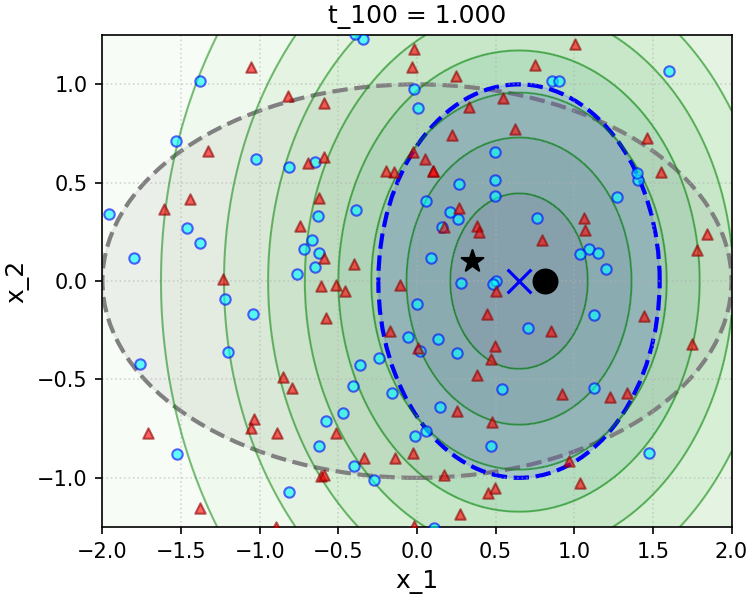
\includegraphics[width=\linewidth]{\toplevelprefix/chapters/chapter6/figs/samples_step_000_t_100_largenoise.png}
    \end{subfigure}
    \hfill
    \begin{subfigure}{0.32\textwidth}
      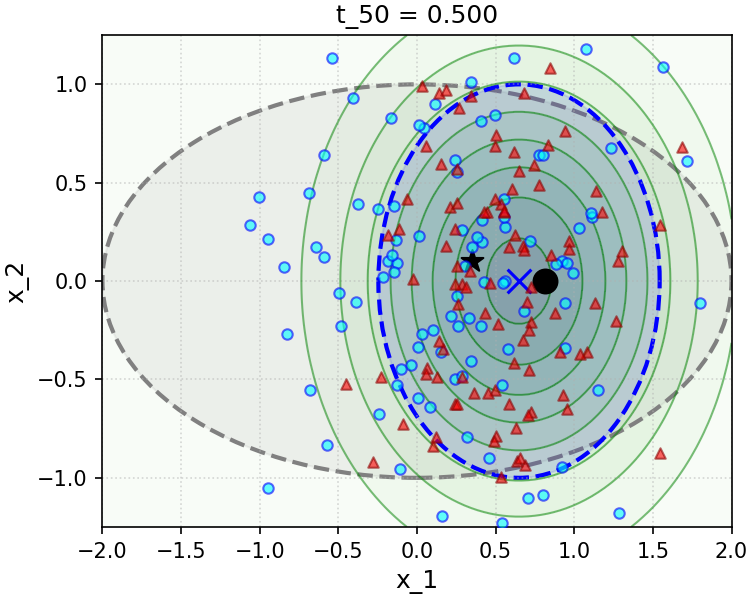
\includegraphics[width=\linewidth]{\toplevelprefix/chapters/chapter6/figs/samples_step_050_t_50_largenoise.png}
    \end{subfigure}
    \hfill
    \begin{subfigure}{0.32\textwidth}
      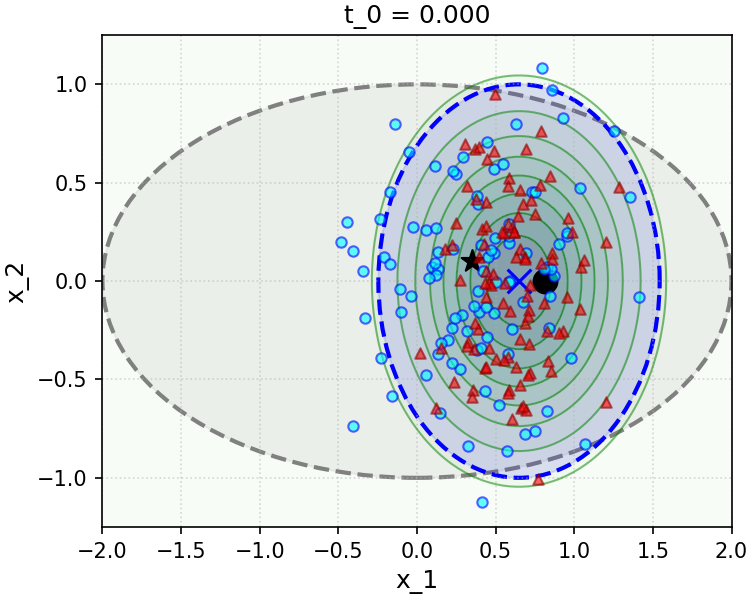
\includegraphics[width=\linewidth]{\toplevelprefix/chapters/chapter6/figs/samples_step_100_t_0_largenoise.png}
    \end{subfigure}

    \vspace{2mm} %

    \begin{subfigure}{0.32\textwidth}
      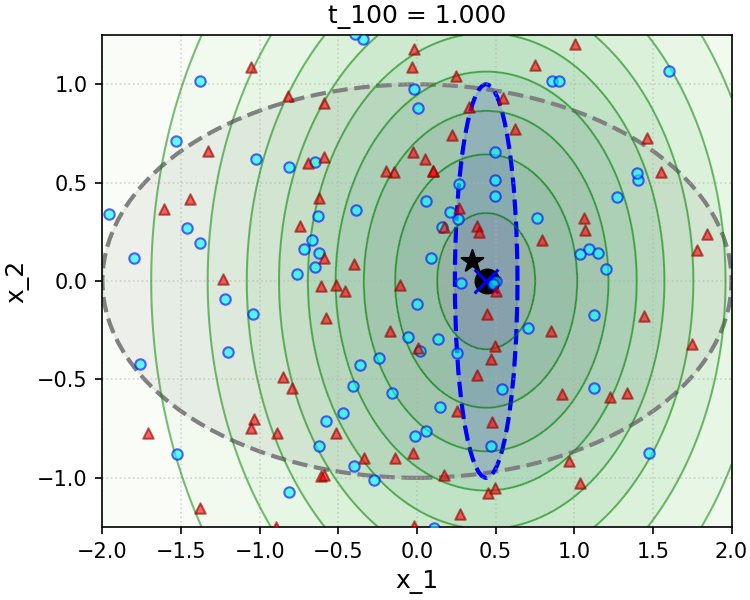
\includegraphics[width=\linewidth]{\toplevelprefix/chapters/chapter6/figs/samples_step_000_t_100_smallnoise.png}
    \end{subfigure}
    \hfill
    \begin{subfigure}{0.32\textwidth}
      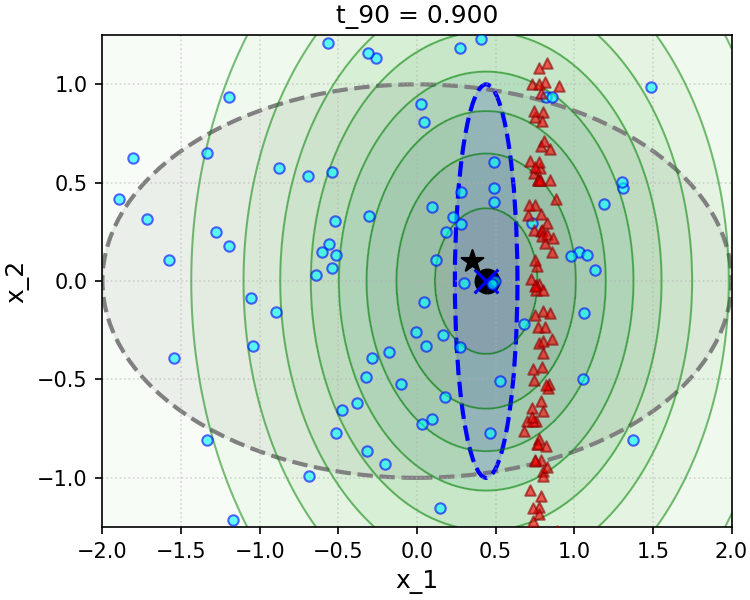
\includegraphics[width=\linewidth]{\toplevelprefix/chapters/chapter6/figs/samples_step_010_t_90_smallnoise.png}
    \end{subfigure}
    \hfill
    \begin{subfigure}{0.32\textwidth}
      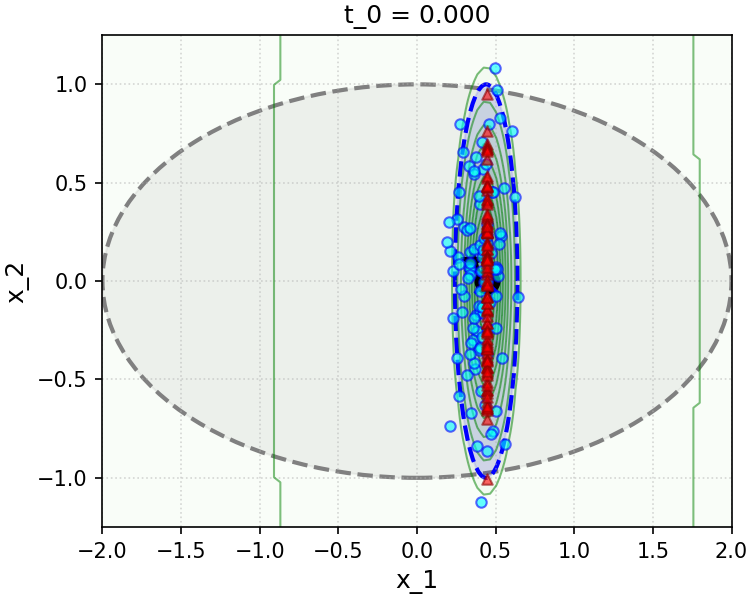
\includegraphics[width=\linewidth]{\toplevelprefix/chapters/chapter6/figs/samples_step_100_t_0_smallnoise.png}
    \end{subfigure}

    \caption{Simulare numerică a configurației de eșantionare condiționată
    \eqref{eq:measurement-matching-observation}, cu date Gaussiene, măsurători
    liniare și zgomot Gaussian. Simulăm $D=2$ și $d=1$, cu $\vSigma
    = \ve_1 \ve_1^\top + \tfrac{1}{4} \ve_2 \ve_2^\top$, $\vmu = \Zero$ și
    $\vA = \ve_1^\top$. Semnalul de bază $\vx$ este marcat cu o stea neagră,
    iar măsurătoarea $\vy$ este marcată cu un cerc negru.
    Fiecare grafic individual corespunde unei valori diferite a timpului de eșantionare
    $t_{\ell}$, cu rânduri diferite corespunzând nivelurilor diferite de zgomot de observație
    $\sigma^2$.
    În fiecare grafic, matricea de covarianță a $\vx$ este trasată în gri, matricea
    de covarianță posterioară și media posterioară a $p_{\vx \mid \vy}$ sunt
    trasate în albastru (cu media posterioară marcată cu un ``x'' albastru), iar
    contururile pentru $p_{\vx_{t_{\ell}} \mid \vy}$ sunt desenate în verde. Hiperparametrii
    eșantionatorului sunt $T=1$, $L=100$ și desenăm $100$
    de eșantioane independente pentru a inițializa eșantionatoarele. Eșantionatoarele sunt implementate
    cu denoiser-ele în formă închisă derivate în
    \Cref{example:denoising-conditional-gaussian}, cu cele care folosesc
    aproximarea
    \eqref{eq:conditional-posterior-measurementmatching-gaussian-case-dps-approx}
    marcate cu triunghiuri roșii și cele care folosesc denoiser-ul posterior condiționat
    exact marcate cu cercuri albastre.
    \textbf{Sus:} Pentru zgomot de observație mare $\sigma = 0.5$, atât
    denoiser-ul posterior condiționat exact, cât și cel aproximativ fac o treabă bună de
    convergență către posteriorul $p_{\vx \mid \vy}$. Timpul de eșantionare (corespunzând
    timpului în ``procesul direct'', deci timpii mai mari înseamnă zgomot mai mare)
    scade de la stânga la dreapta. Dinamica de convergență pentru termenul exact și
    aproximativ de potrivire a măsurătorii sunt similare. \textbf{Jos:} Pentru
    zgomot de observație mai mic $\sigma = 0.1$,
    termenul aproximativ de potrivire a măsurătorii duce la o distorsiune extremă în eșantionator
    (triunghiuri roșii): eșantioanele converg rapid către un subspațiu afin
    de puncte care sunt consistente, modulo o anumită contracție de la denoiser-ul mediei posterioare,
    cu adevărul de bază măsurat, iar iterațiile ulterioare de eșantionare sunt
    incapabile să recupereze varianța posterioară pierdută de-a lungul acestei dimensiuni. Observați
    că timpi diferiți $t_{\ell}$ sunt reprezentați în rândul de jos, comparativ cu
    rândul de sus, pentru a arăta colapsul rapid al aproximării către
    posterior de-a lungul dimensiunii măsurătorii.}
    \label{fig:conditional_sampling_computational_gaussian}
  \end{figure}

  \Cref{eq:conditional-posterior-measurementmatching-gaussian-case-dps-approx}
  este, desigur, o consecință directă a calculelor noastre de mai sus. Totuși, observați
  că dacă interpretăm direct această aproximare, este \textit{ab initio}
  tractabilă: verosimilitatea $p_{\vy \mid \vx} = \cN(\vA\vx, \sigma^2 \vI)$ este
  o distribuție Gaussiană simplă centrată la observație, iar
  aproximarea termenului de potrivire a măsurătorii la care ajungem poate fi
  interpretată ca simpla evaluare a log-verosimilității la așteptarea
  condiționată $\bE[\vx \mid \vx_t = \vxi]$, apoi luarea gradienților cu privire
  la $\vxi$ (și retropropagarea prin așteptarea condiționată, care este
  dată aici de \Cref{eq:posterior-denoiser-gaussian-case}).
  Cu toate acestea, observați că aproximarea din
  \Cref{eq:conditional-posterior-measurementmatching-gaussian-case-dps-approx}
  necesită $t \ll \sqrt{\lambda_{\min}(\vSigma)}$ și că nu este niciodată precisă
  în general când această condiție nu este îndeplinită, chiar în această setare Gaussiană.

  Pentru a obține o perspectivă asupra efectului aproximării convenabile
  \eqref{eq:conditional-posterior-measurementmatching-gaussian-case-dps-approx},
  implementăm și simulăm un experiment numeric simplu în
  setarea Gaussiană în \Cref{fig:conditional_sampling_computational_gaussian}. 
  Eșantionatorul pe care îl implementăm este o implementare directă a schemei simple
  \eqref{eq:denoising-iteration-basic} pe care am dezvoltat-o în \Cref{ch:compression}
  și am reamintit-o mai sus, folosind denoiser-ul posterior condiționat adevărat, adică
  \Cref{eq:conditional-posterior-denoiser-gaussian-case} (rândul de sus din
  \Cref{fig:conditional_sampling_computational_gaussian}), și 
  aproximarea convenabilă a acestui denoiser făcută cu descompunerea
  \eqref{eq:posterior-sampling-denoiser-decomposition}, denoiser-ul posterior
  \eqref{eq:posterior-denoiser-gaussian-case} și aproximarea de
  potrivire a măsurătorii
  \eqref{eq:conditional-posterior-measurementmatching-gaussian-case-dps-approx}
  (rândul de jos din \Cref{fig:conditional_sampling_computational_gaussian}).
  Vedem că chiar și în setarea Gaussiană simplă, aproximarea termenului de
  potrivire a măsurătorii pe care am făcut-o nu este lipsită de
  dezavantaje---specific, la niveluri mici de zgomot $\sigma^2 \ll 1$, aceasta duce la
  colapsul rapid al varianței distribuției de eșantionare de-a lungul direcțiilor
  care sunt paralele cu rândurile operatorului de măsurare liniar $\vA$, care
  nu poate fi corectat de iterațiile ulterioare de eșantionare. Putem intui aceasta din
  aproximarea
  \eqref{eq:conditional-posterior-measurementmatching-gaussian-case-dps-approx}
  și definiția iterației de denoising
  \eqref{eq:denoising-iteration-basic}, dată
  \Cref{eq:posterior-sampling-denoiser-decomposition}: pentru $\sigma^2 \ll 1$,
  pașii timpurii de eșantionare efectiv fac pași de coborâre gradient cu un
  pas foarte mare pe verosimilitate, prin
  \Cref{eq:conditional-posterior-measurementmatching-gaussian-case-dps-approx},
  ceea ce face ca distribuția de eșantionare să rămână ``blocată'' într-o stare colapsată.

\end{example}


\Cref{example:denoising-conditional-gaussian} sugerează o aproximare convenabilă
pentru termenul de potrivire a măsurătorii
\eqref{eq:conditional-posterior-measurementmatching-gaussian-case-dps-approx},
care poate fi făcută dincolo de setarea Gaussiană a exemplului. Pentru a
motiva această aproximare într-o generalitate mai mare, observați că
prin independența condiționată a $\vy$ și $\vx_t$ date $\vx$, putem scrie
\begin{equation}
  p_{\vy \mid \vx_t}(\vnu \mid \vxi)
  =
  \int p_{\vy \mid \vx}(\vnu \mid \vxi') p_{\vx \mid \vx_t}(\vxi' \mid \vxi)
  \odif  \vxi'.
\end{equation}
Formal, când posteriorul $p_{\vx\mid \vx_t}$ este o funcție delta centrată la
media sa $\bE[\vx \mid \vx_t=\vxi]$, aproximarea
\eqref{eq:conditional-posterior-measurementmatching-gaussian-case-dps-approx} este
exactă. Mai general, când posteriorul $p_{\vx \mid \vx_t}$ este foarte
concentrat în jurul mediei sale, aproximarea
\eqref{eq:conditional-posterior-measurementmatching-gaussian-case-dps-approx} este
precisă. Aceasta este valabilă, de exemplu, pentru $t$ suficient de mic, ceea ce am văzut
explicit în setarea Gaussiană din
\Cref{example:denoising-conditional-gaussian}.
Deși simularea numerică din
\Cref{fig:conditional_sampling_computational_gaussian} sugerează că această
aproximare nu este lipsită de avertismente în anumite regimuri, s-a dovedit a fi
o bază de referință fiabilă în practică, după ce a fost propusă de Chung et al.\ ca
``Eșantionare Posterioară prin Difuzie'' (DPS) \cite{chung2023diffusion}.
În plus, există chiar abordări principiale și generalizabile pentru a o îmbunătăți prin
încorporarea unor estimări mai bune ale varianței posterioare (care se dovedesc a fi
exacte în setarea Gaussiană din \Cref{example:denoising-conditional-gaussian}),
pe care le discutăm mai departe în rezumatul de la sfârșitul capitolului.

Astfel, cu aproximarea DPS, ajungem la următoarea aproximare pentru
denoiser-ele posterioare condiționate $\bE[\vx \mid \vy, \vx_t]$, prin
\Cref{eq:posterior-sampling-denoiser-decomposition}:
\begin{equation}
  \bE[ \vx \mid \vx_t=\vxi, \vy=\vnu]
  \approx
  \bE[\vx \mid \vx_t=\vxi] 
  + t^2 \nabla_{\vxi} \log p_{\vy \mid \vx}(\vnu \mid \bE[\vx \mid \vx_t = \vxi]).
  \label{eq:posterior-sampling-denoiser-decomposition-dps}
\end{equation}
Și, pentru o rețea neuronală sau alt model $\bar{\vx}_{\theta}(t, \vxi)$ 
antrenat ca în \Cref{sub:compression_denoising} pentru a aproxima denoiser-ele
$\bE[\vx \mid \vx_t = \vxi]$ pentru fiecare $t \in [0, T]$, ajungem la denoiser-ele
posterioare condiționate învățate
\begin{equation}
  \bar{\vx}_{\theta}(t, \vxi, \vnu) 
  = \bar{\vx}_{\theta}(t, \vxi)
  + t^2 \nabla_{\vxi} \log p_{\vy \mid \vx}(\vnu \mid \bar{\vx}_{\theta}(t,
  \vxi)).
  \label{eq:posterior-sampling-denoiser-learned-dps}
\end{equation}
Observați că aproximarea
\eqref{eq:posterior-sampling-denoiser-decomposition-dps} este validă pentru modele
directe arbitrare $h$ în
modelul de observație \eqref{eq:measurement-matching-observation}, inclusiv
$h$ neliniar, și chiar pentru
modele arbitrare de zgomot pentru care o expresie clară pentru verosimilitatea $p_{\vy
\mid \vx}$ este cunoscută. Într-adevăr, în cazul zgomotului Gaussian, avem
\begin{equation}
  p_{\vy \mid \vx}(\vnu \mid \vxi)
  \propto
  \exp\left(
    -\frac{1}{2\sigma^2} \norm*{ h(\vxi) - \vnu }_2^2
  \right).
\end{equation}
Prin urmare, evaluarea părții drepte a
\eqref{eq:posterior-sampling-denoiser-learned-dps}
necesită doar
\begin{enumerate}
  \item Un denoiser pre-antrenat $\bar{\vx}_{\theta}(t, \vxi)$ pentru distribuția datelor $p$
    (a $\vx)$, învățat ca în \Cref{sub:compression_denoising} prin
    \Cref{alg:learning_denoiser};
  \item Acces la trecerea directă și inversă la modelul direct $h$ pentru
    măsurători \eqref{eq:measurement-matching-observation};
  \item O trecere directă și inversă prin $\bar{\vx}_{\theta}(t, \vxi)$, care poate fi evaluată
    eficient folosind (să zicem) retropropagarea.
\end{enumerate}

\begin{algorithm}
  \caption{Eșantionare condiționată sub măsurători
  \eqref{eq:measurement-matching-observation}, cu un denoiser necondiționat și DPS.}
	\label{alg:iterative_denoising_conditional_DPS}
	\begin{algorithmic}[1]
		\Require{O listă ordonată de pași de timp \(0 \leq t_{0} < \cdots < t_{L} \leq T\) de folosit pentru eșantionare.}
    \Require{Un denoiser necondiționat \(\bar{\vx}_{\theta} \colon
    \{t_{\ell}\}_{\ell = 1}^{L} \times \R^{D} \to \R^{D}\) pentru $p_{\vx}$.}
    \Require{Realizarea măsurătorii $\vnu$ a $\vy$ (\Cref{eq:measurement-matching-observation}) pe care să condiționăm.}
    \Require{Modelul direct $h : \bR^D \to \bR^d$ și varianța zgomotului de măsurare
    $\sigma^2 > 0$.}
		\Require{Funcțiile de scară și nivel de zgomot \(\alpha, \sigma \colon \{t_{\ell}\}_{\ell = 0}^{L} \to \R_{\geq 0}\).}
    \Ensure{Un eșantion \(\hat{\vx}\), aproximativ din \(p_{\vx \mid \vy}\).}
    \Function{DDIMSamplerConditionalDPS}{$\bar{\vx}_{\theta}, \vnu, h, \sigma^2,
    (t_{\ell})_{\ell = 0}^{L}$}
		\State{Inițializează \(\hat{\vx}_{t_{L}} \sim\) distribuție aproximativă a \(\vx_{t_{L}}\)} \Comment{VP \(\implies \dNorm(\vzero, \vI)\), VE \(\implies \dNorm(\vzero, t_{L}^{2}\vI)\).}
		\For{\(\ell = L, L - 1, \dots, 1\)}
		\State{Calculează
			\begin{equation*}
				\hat{\vx}_{t_{\ell - 1}} \doteq \frac{\sigma_{t_{\ell
        - 1}}}{\sigma_{t_{\ell}}}\hat{\vx}_{t_{\ell}} + \bp{\alpha_{t_{\ell
        - 1}} - \frac{\sigma_{t_{\ell
        - 1}}}{\sigma_{t_{\ell}}}\alpha_{t_{\ell}}}\left(
        \bar{\vx}_{\theta}(t_{\ell}, \hat{\vx}_{t_{\ell}})
        - \frac{\sigma_{t_{\ell}}^2}{2\alpha_{t_\ell}\sigma^2}
        \nabla_{\vxi}\left[ \norm*{h( \bar{\vx}_{\theta}(t_{\ell}, \vxi)
        ) - \vnu}_2^2 \right]\biggl|_{\vxi = \hat{\vx}_{t_{\ell}}}\biggr.
        \right)
			\end{equation*}
		}
		\EndFor
		\State{\Return{\(\hat{\vx}_{t_{0}}\)}}
		\EndFunction
	\end{algorithmic}
\end{algorithm}

Combinând această schemă cu implementarea de bază a eșantionării necondiționate pe care am
dezvoltat-o în \Cref{sub:compression_denoising}, obținem un algoritm practic pentru
eșantionarea condiționată a posteriorului $p_{\vx \mid \vy}$ date măsurătorile
care urmează \eqref{eq:measurement-matching-observation}.
\Cref{alg:iterative_denoising_conditional_DPS} înregistrează această schemă
pentru cazul
zgomotului de observație Gaussian cu deviație standard cunoscută $\sigma$, cu modificări minore
pentru a extinde la un proces general de zgomot, ca în
\Cref{eq:gen_additive_gaussian_noise_model} și discuția înconjurătoare din
\Cref{ch:compression} (discuția noastră de mai sus a făcut alegerile simplificatoare $\alpha_t = 1$, $\sigma_t = t$ și
$t_{\ell} = T\ell / L$, ca pentru \Cref{eq:denoising-iteration-basic} în
\Cref{sub:compression_denoising}).



\subsection{Generarea Pozei Corpului Condiționată de Cap și Mâini}\label{sub:ego-allo}
Acest tip de
problemă de estimare sau generare condiționată apare destul de natural în multe
aplicații practice. 
O problemă tipică de acest gen este cum să estimăm și să generăm poza corpului și gestul mâinilor condiționat de o poză dată a capului și imagini egocentrice, așa cum este ilustrat în Figura \ref{fig:pose-teaser}. Aceasta este adesea problema pe care trebuie să o rezolvăm când cineva poartă un dispozitiv montat pe cap, cum ar fi Vision Pro de la Apple sau Project Aria de la Meta. Poza întregului corp și gestul mâinilor trebuie inferate astfel încât să putem folosi informația pentru a controla obiecte virtuale cu care persoana interacționează.
\begin{figure*}[t]
  \centering
  \includegraphics[width=\linewidth]{\toplevelprefix/chapters/chapter6/figs/pose-teaser.pdf}
    \caption{
Un sistem care estimează înălțimea, poza și parametrii mâinilor corpului uman (mijloc), condiționat de pozele SLAM egocentrice și imagini (stânga). Ieșirile captează acțiunile purtătorului în cadrul de referință alocentric al scenei, pe care îl vizualizăm aici cu reconstrucții 3D (dreapta).
  }
  \label{fig:pose-teaser}

\end{figure*}

Observați că în acest caz, avem doar poza capului furnizată de dispozitiv și un câmp vizual foarte limitat pentru o parte din mâini și membrele superioare. Poza restului corpului trebuie să fie ``inferată'' sau ``completată'' pe baza unor astfel de informații parțiale. Singura modalitate prin care se poate estima poza corpului în timp este învățând distribuția comună a secvențelor de poză a capului și corpului în avans și apoi eșantionând această distribuție prioră condiționată de intrările parțiale în timp real. Figura \ref{fig:pose-method} conturează un sistem numit EgoAllo \cite{yi2024egoallo} pentru a rezolva această problemă bazat pe un model de difuzie-denoising condiționat învățat.

\begin{figure*}[t]
  \centering
  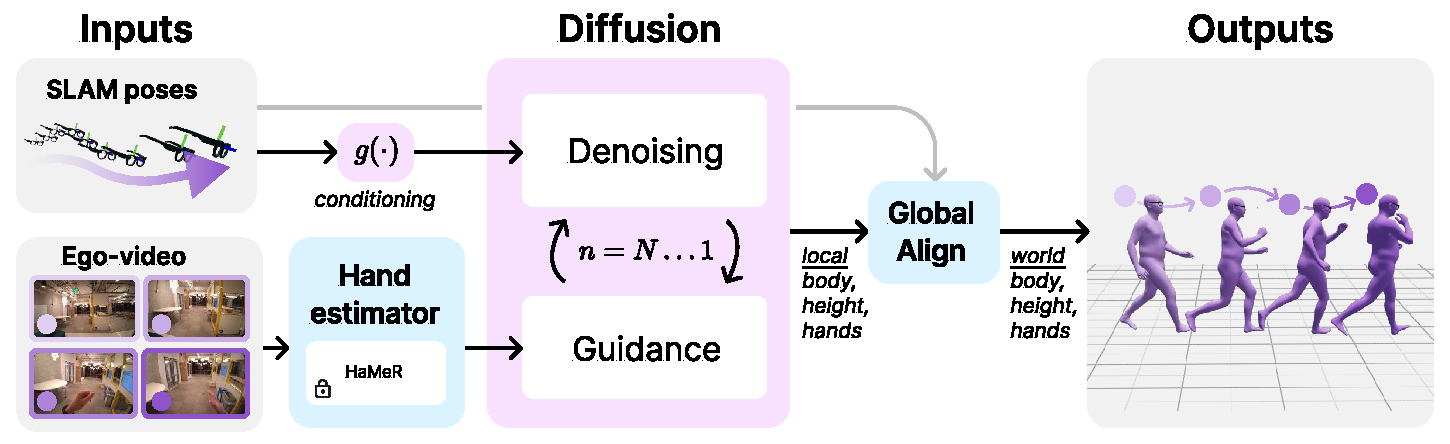
\includegraphics[width=\linewidth]{\toplevelprefix/chapters/chapter6/figs/pose-method.pdf}
\caption{
    \textbf{Prezentare generală a componentelor tehnice ale EgoAllo \cite{yi2024egoallo}.}
    Un model de difuzie este pre-antrenat care poate genera secvențe de poză a corpului bazate pe parametri locali ai corpului (mijloc).
    O parametrizare invariantă $g(\cdot)$ a pozelor SLAM (stânga) este folosită pentru a condiționa modelul de difuzie. Acestea pot fi plasate în cadrul de coordonate global prin aliniere globală la pozele de intrare.
    Când sunt disponibile, videoclipurile egocentrice sunt folosite pentru detectarea mâinilor (stânga) prin HaMeR~\cite{pavlakos2023reconstructing}, care pot fi încorporate în eșantioane prin ghidare de gestul generat.
  }
  \label{fig:pose-method}
\end{figure*}


Figura \ref{fig:comparison} compară unele secvențe de mișcare adevărate cu rezultatele eșantionate generate de EgoAllo. Deși figura arată un rezultat pentru fiecare secvență de poză a capului de intrare, rulări diferite pot genera secvențe diferite de poză a corpului care sunt consistente cu poza capului dată, toate extrase din distribuția secvențelor naturale de mișcare a întregului corp.
\begin{figure}[t]
\centering
\begin{subfigure}{0.45\textwidth}
  \centering
  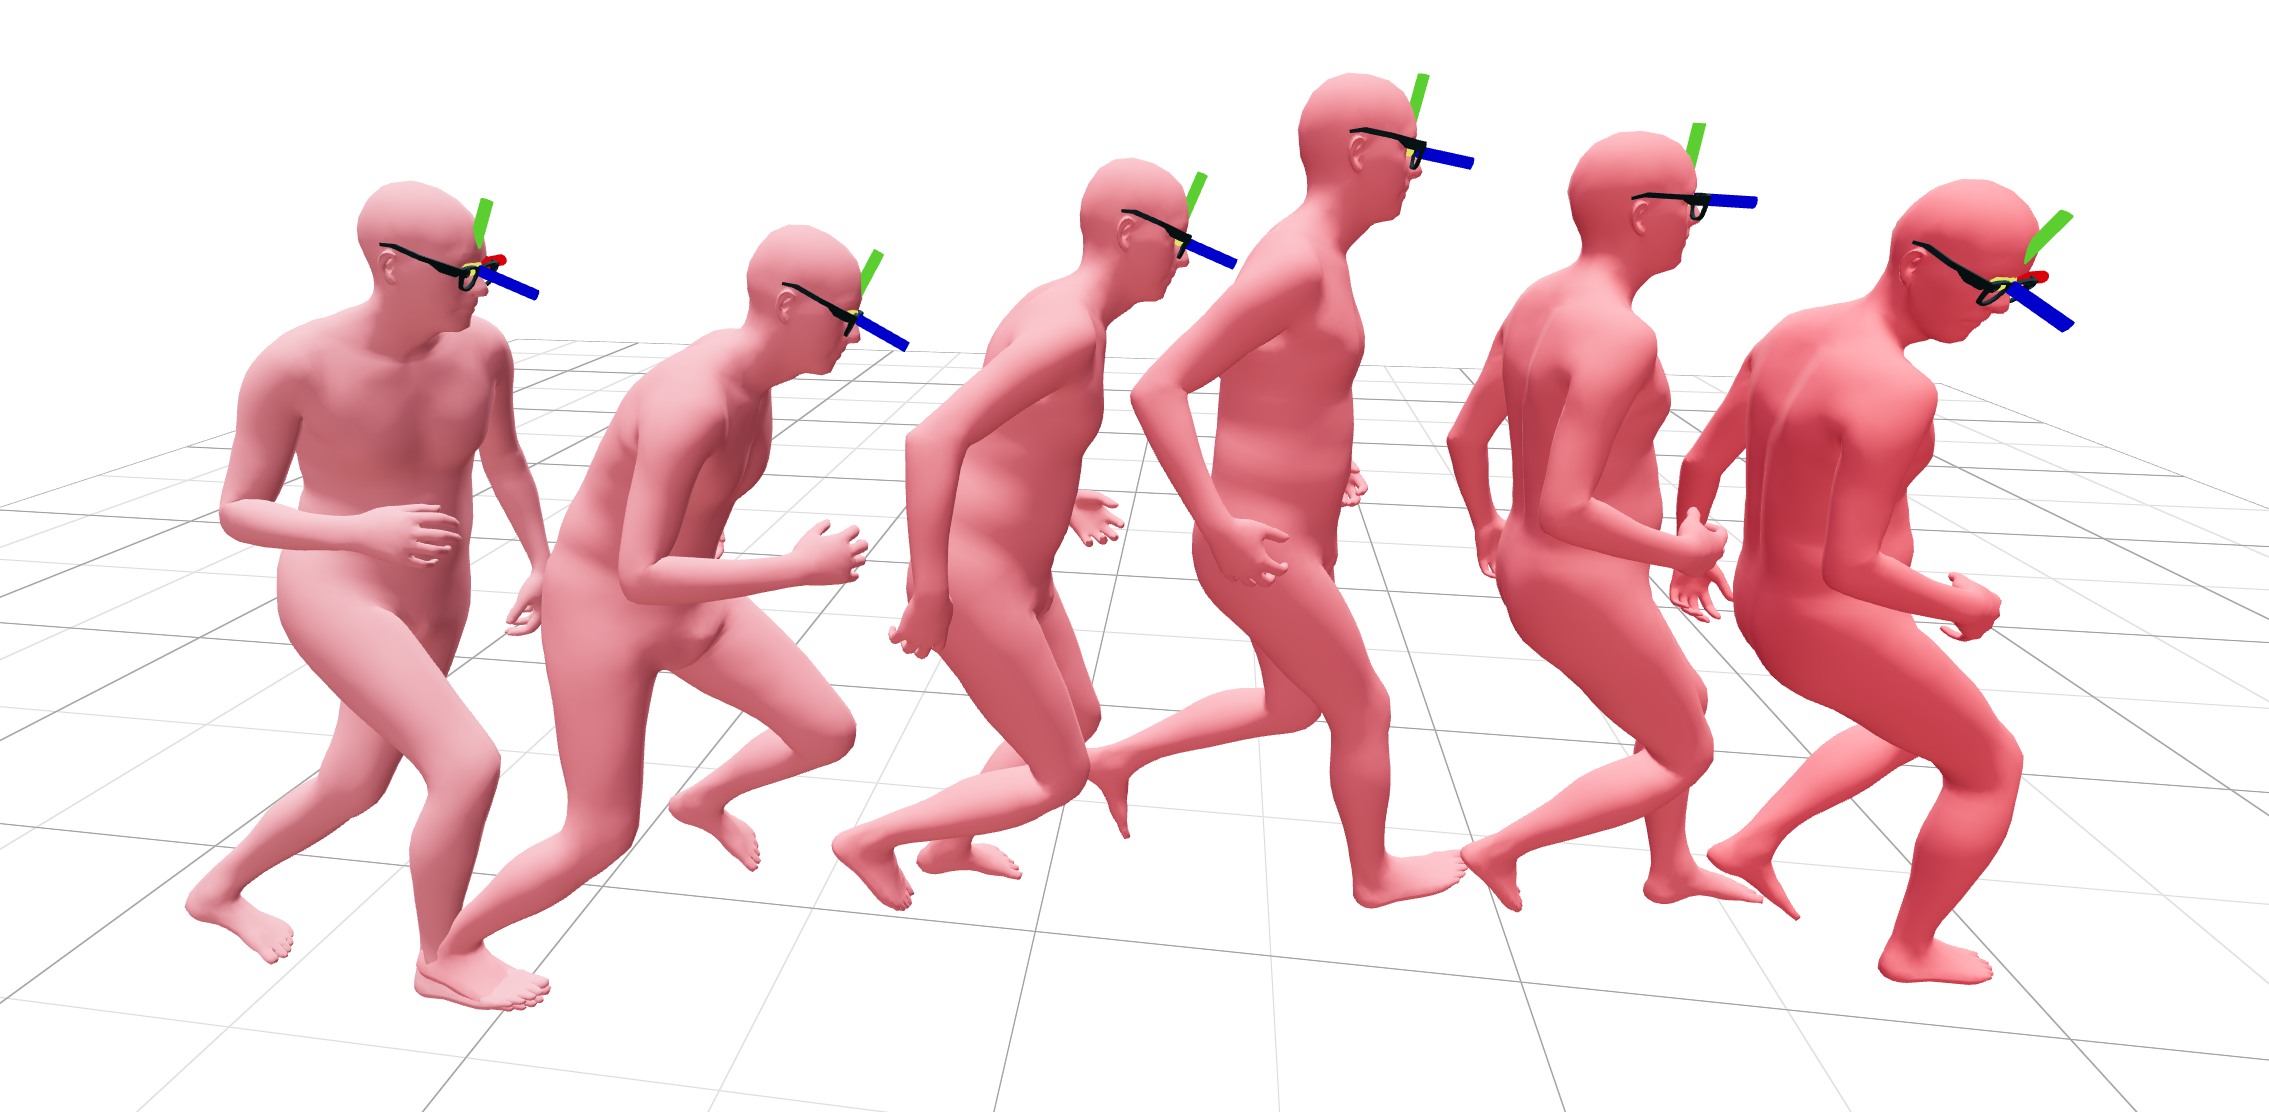
\includegraphics[width=\linewidth]{\toplevelprefix/chapters/chapter6/figs/qual0_gt.png}
  \caption{\centering Adevăr de bază}
\end{subfigure}
\hfill
\begin{subfigure}{0.45\textwidth}
  \centering
  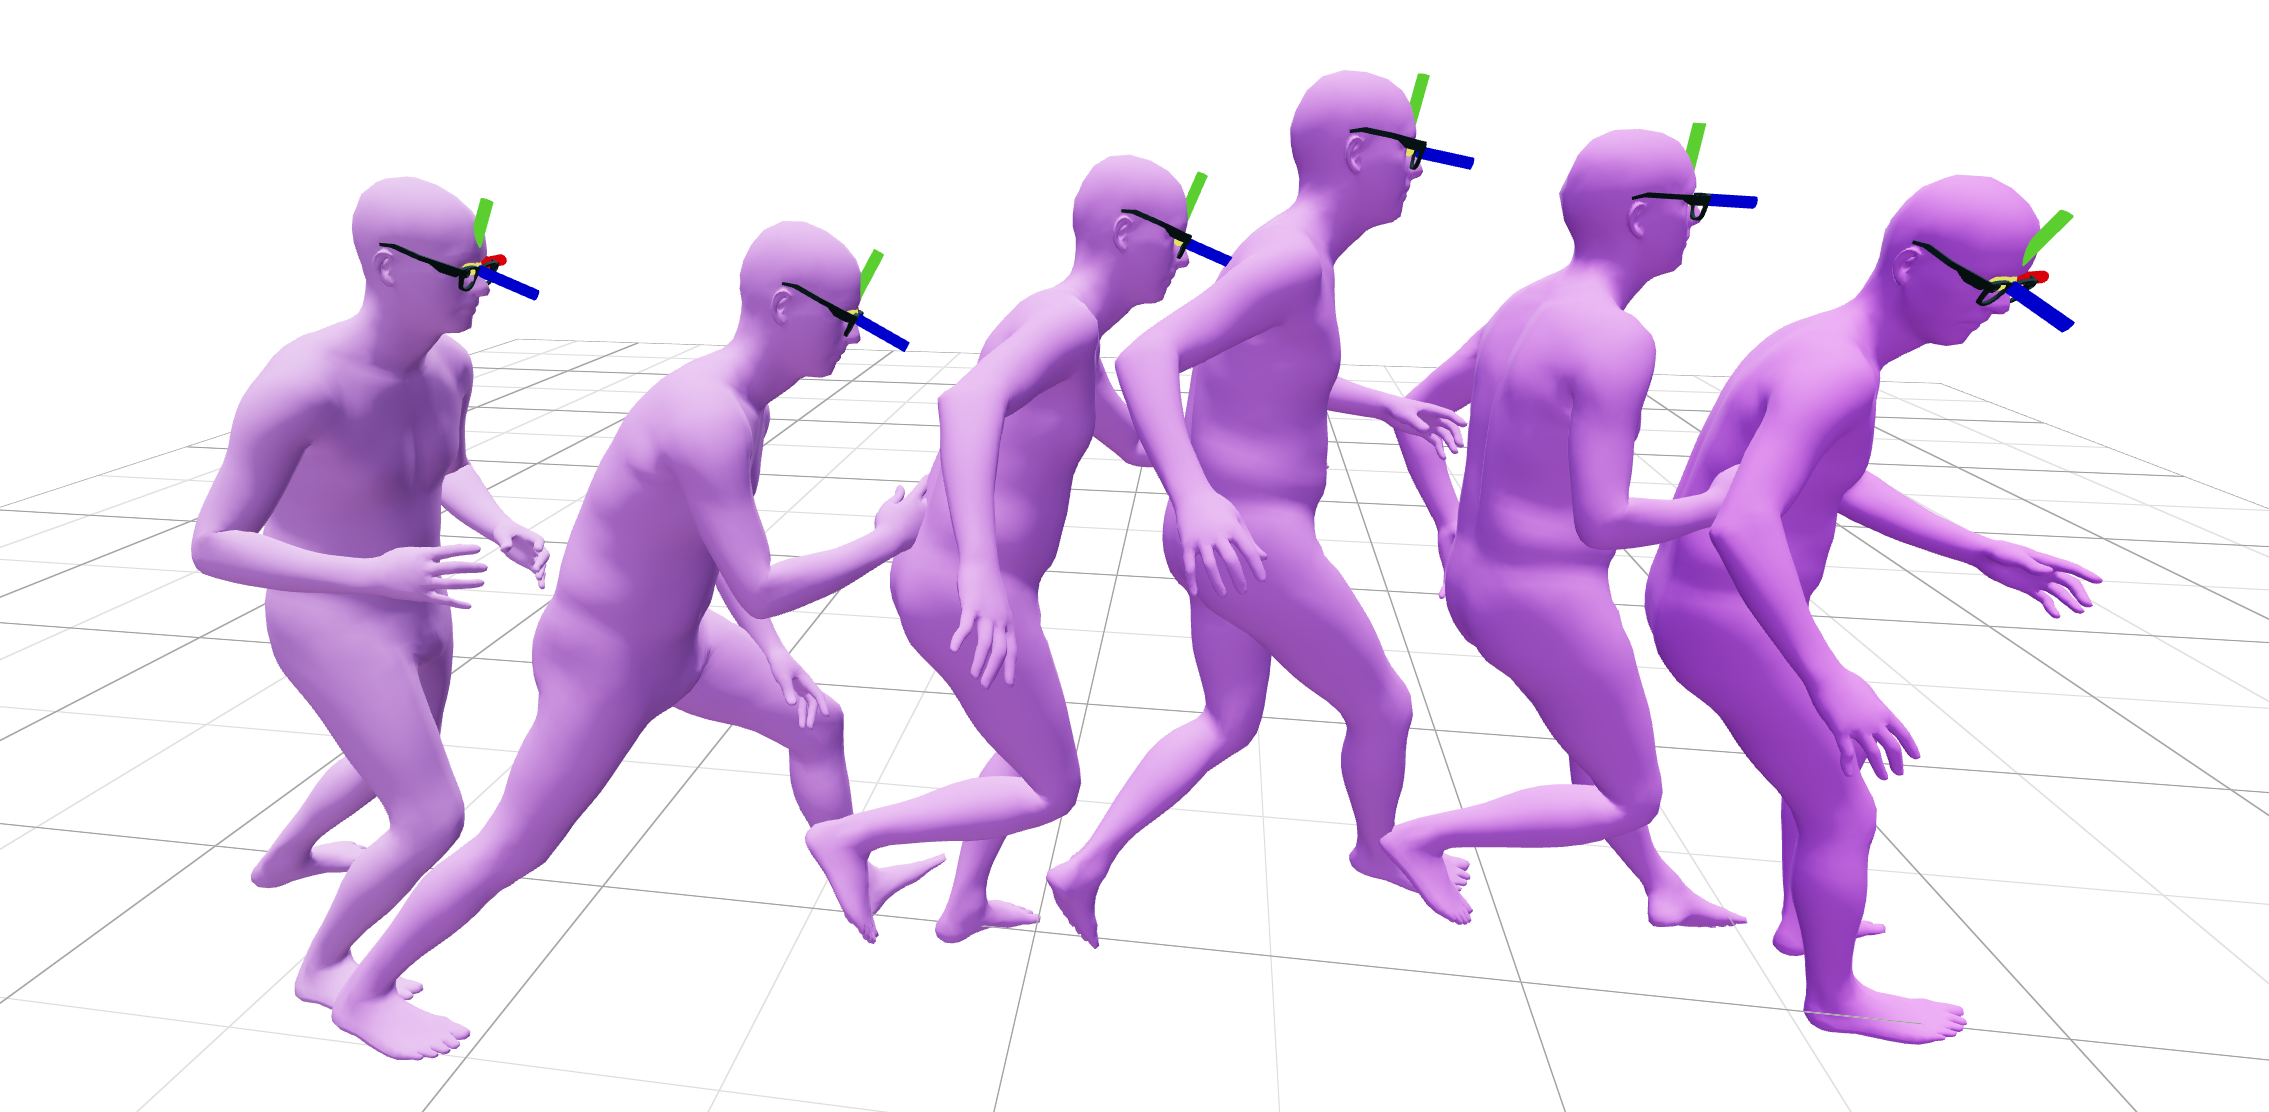
\includegraphics[width=\linewidth]{\toplevelprefix/chapters/chapter6/figs/qual0_ours.png}
  \caption{EgoAllo}
\end{subfigure}

\begin{subfigure}{0.45\textwidth}
  \centering
  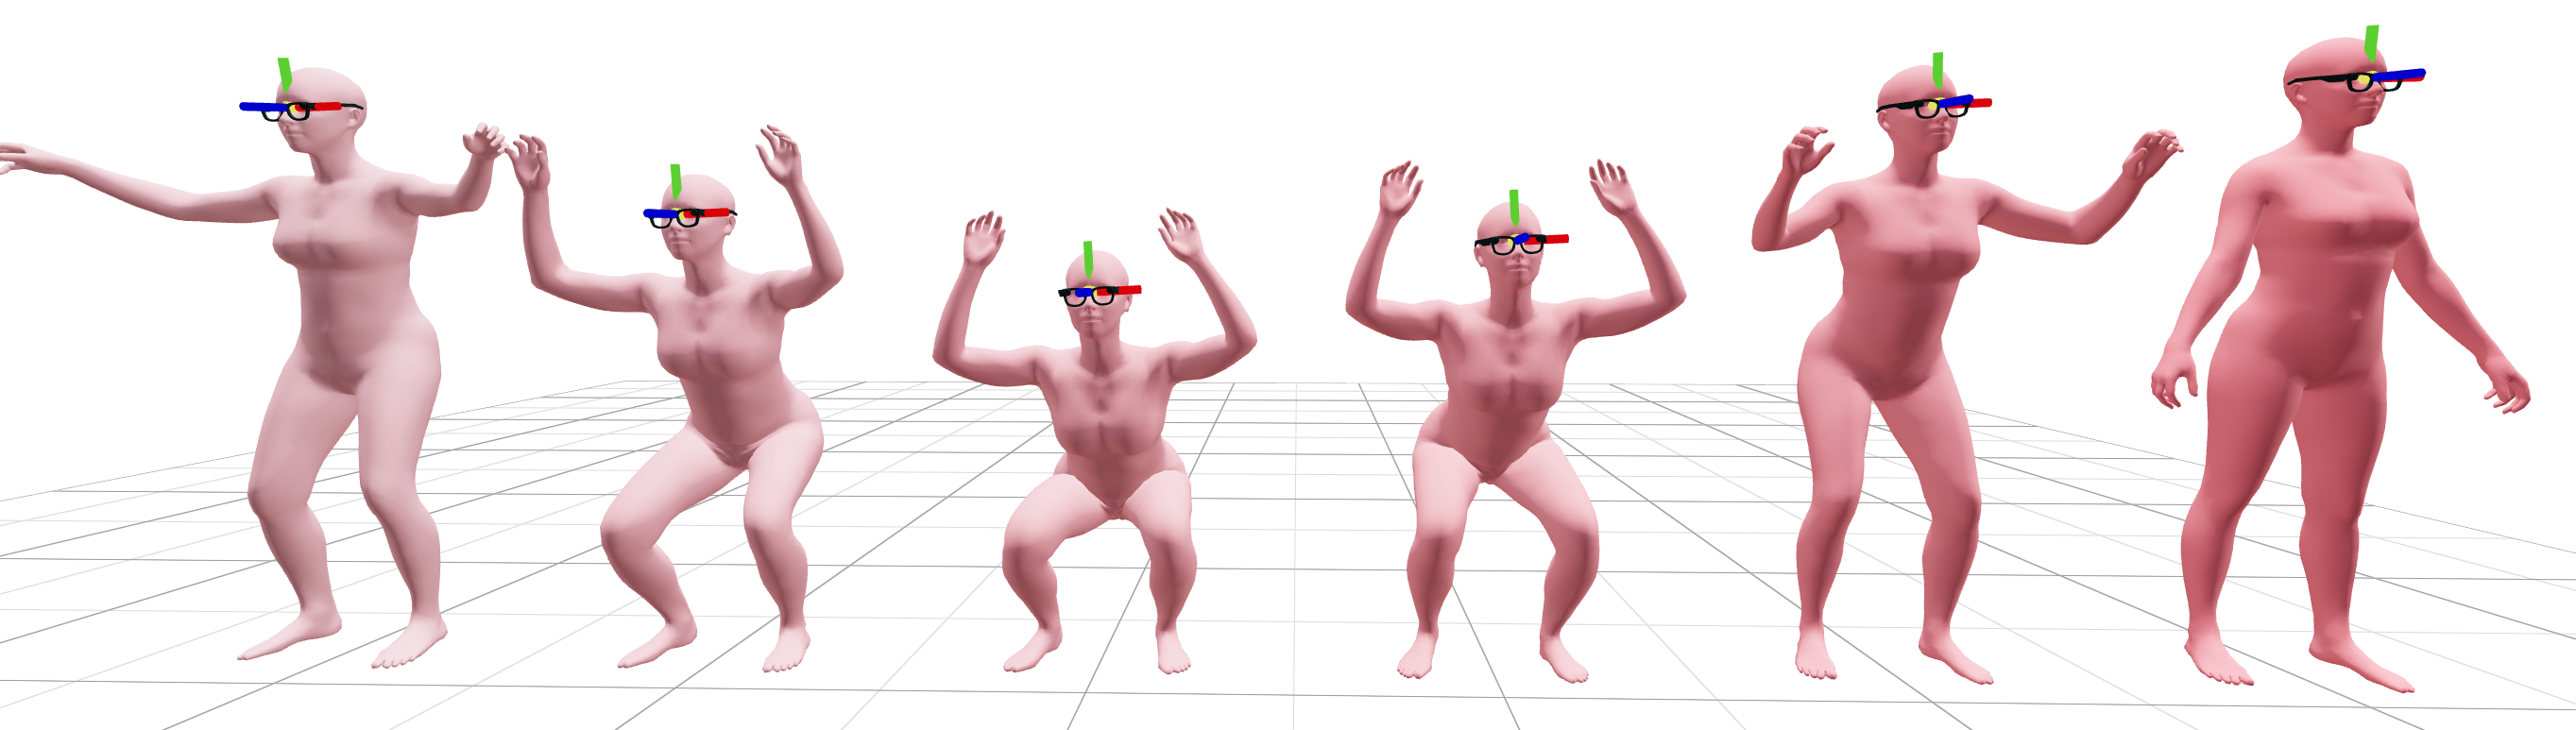
\includegraphics[width=\linewidth]{\toplevelprefix/chapters/chapter6/figs/qual1_gt.png}
  \caption{\centering Adevăr de bază}
\end{subfigure}
\hfill
\begin{subfigure}{0.45\textwidth}
  \centering
  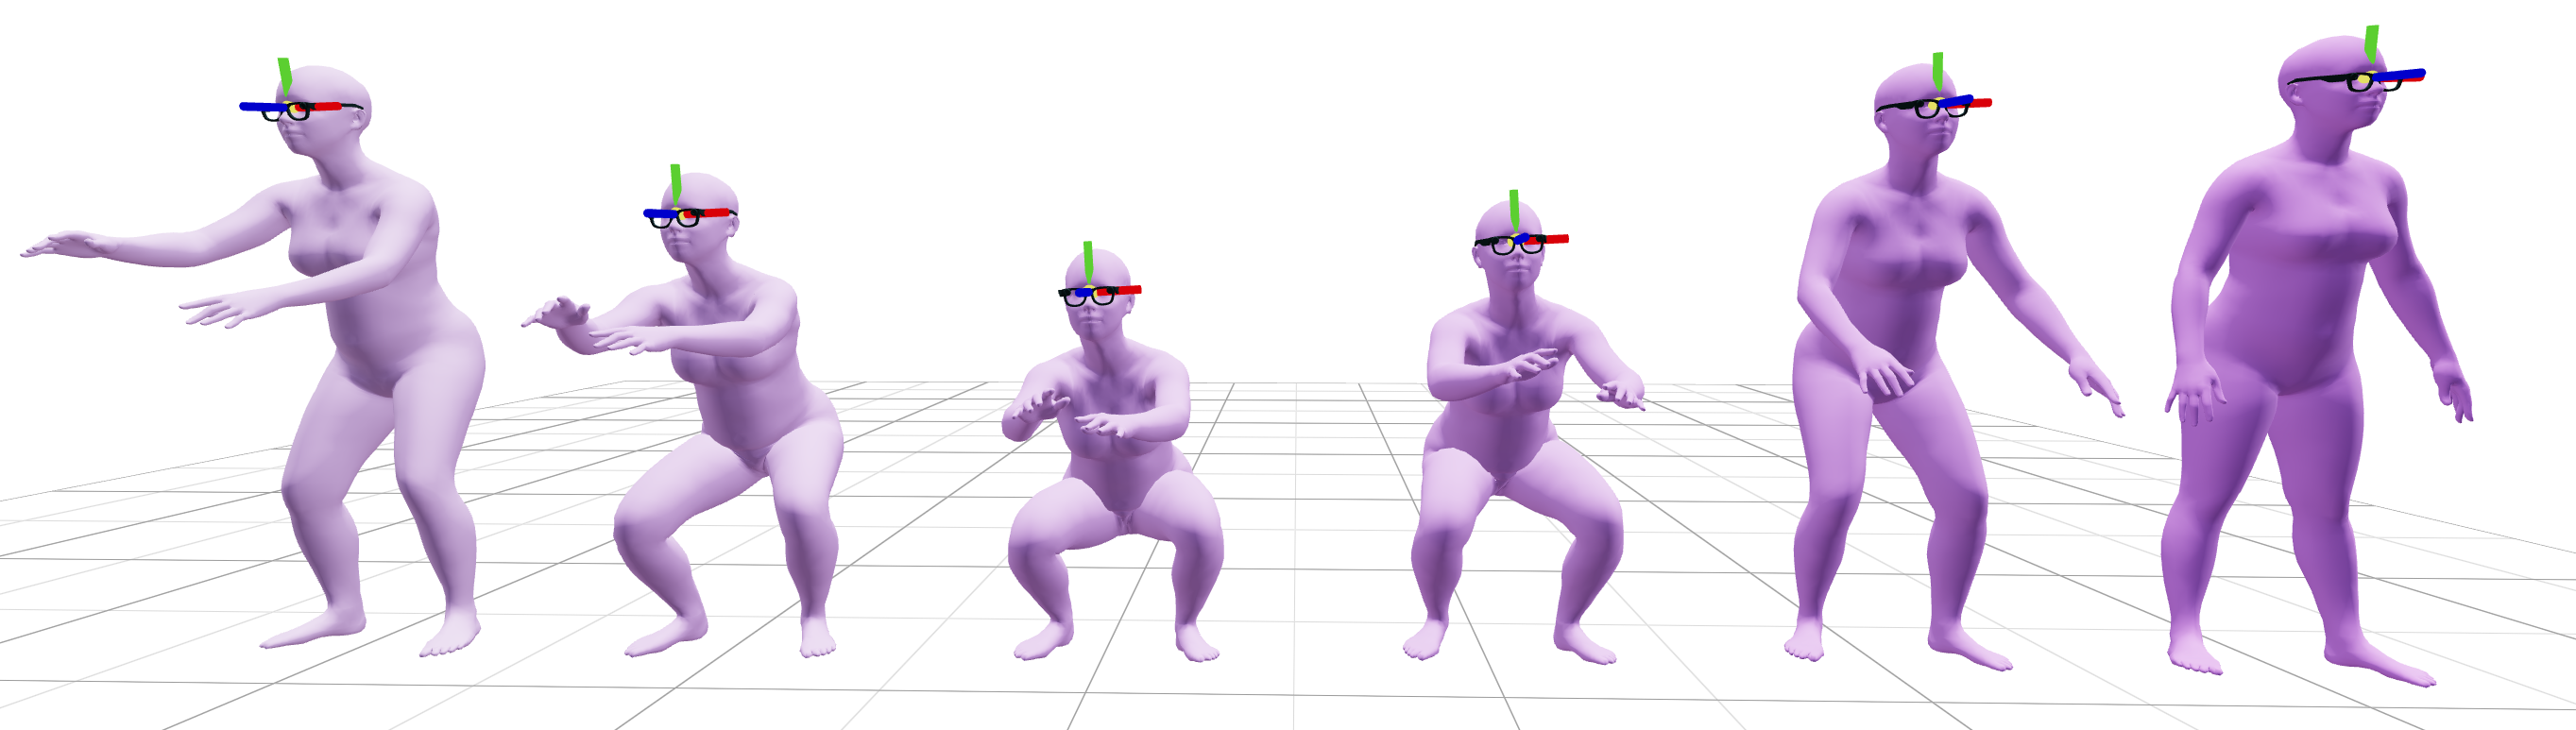
\includegraphics[width=\linewidth]{\toplevelprefix/chapters/chapter6/figs/qual1_ours.png}
  \caption{EgoAllo}
\end{subfigure}

\caption{
\textbf{Estimarea mișcării umane egocentrice pentru o secvență de alergare (sus) și ghemuit (jos).}
Mișcarea adevărului de bază este comparată cu o ieșire din EgoAllo care este consistentă cu secvența de poză a capului dată. 
}
\label{fig:comparison}
\end{figure}

Strict vorbind, soluția propusă în EgoAllo \cite{yi2024egoallo} nu
impune potrivirea măsurătorii folosind tehnicile introduse mai sus. În schimb,
impune euristic condiția utilizând mecanismul de atenție încrucișată
într-o arhitectură transformer. După cum vom descrie cu mai multă precizie
în setarea datelor pereche în \Cref{sub:text-cond}, există motive să credem că mecanismul
de atenție încrucișată realizează într-un fel aproximativ eșantionarea condiționată
a denoising-ului a posteriori. Credem că tehnicile mai principiale
introduse aici, dacă sunt implementate corespunzător, pot duce la metode mai bune
care îmbunătățesc în continuare estimarea pozei corpului și a gestului mâinilor.

\section{Inferență Condiționată cu Date Pereche și Măsurători}
În multe aplicații practice, nu cunoaștem nici distribuția datelor $\x$ de interes, nici relația explicită dintre date și anumite atribute observate $\y$ ale datelor. Avem doar un set (mare) de eșantioane pereche $(\X, \Y) = \{ (\x_1, \y_1), \ldots, (\x_N, \y_N) \}$ din care trebuie să inferăm distribuția datelor și o mapare care modelează relația lor:
\begin{equation}
  h: \x \mapsto \y.
\end{equation}

Problema clasificării imaginilor poate fi văzută ca un astfel de exemplu. Într-un sens, problema de clasificare este să învățăm un codificator compresiv (extrem de cu pierderi) pentru imagini naturale. Să zicem, dată o mostră aleatorie a unei imagini $\x$, am dori să prezicem eticheta sa de clasă $\y$ care corelează cel mai bine conținutul din $\x$. Știm că distribuția imaginilor naturale ale obiectelor este de dimensiune redusă comparativ cu dimensiunea spațiului pixelilor. Din capitolele anterioare, am învățat că, date suficiente eșantioane, în principiu, putem învăța o reprezentare structurată de dimensiune redusă $\z$ pentru $\x$ printr-o codare compresivă învățată:
\begin{equation}
    f: \x \mapsto \z. 
\end{equation}
Reprezentarea $\z$ poate fi văzută și ca un cod învățat (cu pierderi dar structurat) pentru $\x$. Este destul de rezonabil să presupunem că dacă atribuirea clasei $\y$ depinde cu adevărat de structurile de dimensiune redusă ale lui $\x$ și codul învățat $\z$ reflectă cu adevărat astfel de structuri, $\y$ și $\z$ pot fi făcute foarte corelate și, prin urmare, distribuția lor comună $p(\z, \y)$ ar trebui să fie extrem de redusă dimensional. Prin urmare, putem combina cele două coduri dorite $\y$ și $\z$ împreună și încerca să învățăm un codificator combinat:
\begin{equation}
    f: \x \mapsto (\z, \y) 
\end{equation}
unde distribuția comună a $(\z, \y)$ este foarte redusă dimensional.

Din studiul nostru în capitolele anterioare, maparea $f$ este de obicei învățată ca o secvență de operatori de compresie sau denoising în același spațiu. Prin urmare, pentru a valorifica o astfel de familie de operații, putem introduce un vector auxiliar $\vw$ care poate fi văzut ca o estimare aleatorie inițială a etichetei de clasă $\y$. În acest fel, putem învăța o mapare de compresie sau denoising:
\begin{equation}\label{eq:classifier-with-class-token}
    f: (\x, \vw) \mapsto (\z, \y)
\end{equation}
într-un spațiu comun. De fapt, practica comună de a introduce un ``token de clasă'' auxiliar în antrenarea unui transformer pentru sarcini de clasificare, cum ar fi în ViT, poate fi văzută ca învățarea unei astfel de reprezentări prin comprimarea (ratei de codare a) eșantioanelor date (zgomotoase) ale $(\x, \vw)$. Dacă distribuția datelor $\x$ este deja un amestec de Gaussiene (de dimensiune redusă), lucrarea \cite{wright2008classification} a arătat că clasificarea poate fi făcută eficient prin minimizarea directă a {\em lungimii de codare (cu pierderi)} asociată cu eșantioanele date.


\subsection{Generarea de Imagini Condiționată de Clasă}\label{sub:cfg} 
În timp ce un clasificator învățat ne permite să clasificăm o imagine dată $\x$ la
clasa sa corespunzătoare, adesea am dori să generăm o imagine dintr-o clasă dată, prin
eșantionarea distribuției învățate a imaginilor naturale. Într-o anumită măsură, aceasta poate fi
văzută ca problema ``inversă'' a clasificării imaginilor. Fie $p_{\x}$ să denoteze
distribuția imaginilor naturale, să zicem modelată printr-un proces de
difuzie-denoising. Dată o variabilă aleatoare de etichetă de clasă $y \in [K]$ cu realizare $\nu$, să zicem
un ``Măr'', am dori să eșantionăm distribuția condiționată $p_{\x \mid
y}(\,\cdot\, \mid \nu)$ pentru a genera o imagine a unui măr:
\begin{equation}
  \hat{\x} \sim p_{\x\mid \y}(\,\cdot\, \mid \vnu).
\end{equation}
Numim aceasta {\em generare de imagini condiționată de clasă}.

În \Cref{sec:conditioned-decoding}, am văzut cum să folosim paradigma de denoising-difuzie pentru
eșantionarea condiționată din posteriorul $p_{\vx \mid \vy}$ date
măsurători \textit{bazate pe model} $\vy = h(\vx) + \vw$
(\Cref{eq:measurement-matching-observation}), culminând cu
algoritmul DPS (\Cref{alg:iterative_denoising_conditional_DPS}). Acesta este un cadru puternic,
dar nu se aplică problemei de generare de imagini condiționată de clasă (sau text)
de aici, unde un model generativ explicit $h$ pentru
observații/atribute $y$ nu este disponibil din cauza
intractabilității modelării analitice. În această secțiune, vom prezenta tehnici pentru extinderea
eșantionării condiționate la această setare.


Astfel, presupunem acum doar că avem acces la eșantioane din distribuția comună
a $(\vx, y)$:
\begin{equation}
  (\vx, y) \sim p_{\vx, y}.
\end{equation}
Ca în secțiunea anterioară, definim $\vx_t = \alpha_t \vx + \sigma_t \vg$
cu $\vg \sim \cN(\Zero, \vI)$ independent de $(\vx, \vy)$, ca în
\Cref{eq:gen_additive_gaussian_noise_model} în \Cref{ch:compression},
și vom folosi în mod repetat notația $\vxi$ pentru a denota realizările lui $\vx$
și $\vx_t$.

Pentru a continua, observăm că dezvoltarea noastră a eșantionării condiționate sub
măsurători $\vy = h(\vx) + \vw$ a folosit doar explicit
modelul direct $h$ în realizarea aproximării DPS
\eqref{eq:conditional-posterior-measurementmatching-gaussian-case-dps-approx}.
În particular, descompunerea denoiser-ului posterior condiționat
\eqref{eq:posterior-sampling-denoiser-decomposition} \textit{încă este valabilă în
setarea datelor pereche}, în virtutea regulii lui Bayes
și a independenței condiționate a $\vy$ și $\vx_t$ date $\vx$ (reamintiți
\Cref{fig:posterior-sampling-cds}). Astfel putem încă scrie în setarea
datelor pereche
\begin{equation}\label{eq:conditional-denoising-mmse-denoiser-paired-data}
  \bE[ \vx \mid \vx_t=\vxi, y=\nu]
  =
  \bE[\vx \mid \vx_t=\vxi] 
  + \frac{\sigma_t^2}{\alpha_t} 
  \nabla_{\vxi}\log p_{y \mid \vx_t}(\nu\mid \vxi).
\end{equation}
O idee naturală este atunci să implementăm direct termenul de corecție a verosimilității din
\eqref{eq:conditional-denoising-mmse-denoiser-paired-data} folosind o rețea profundă
$f_{\theta_{\mathrm{c}}}$ cu parametri $\theta_{\mathrm{c}}$, ca în
\Cref{eq:classifier-with-class-token}: 
\begin{equation}
  f_{\theta_{\mathrm{c}}} : (t, \vx_t) \mapsto \softmax(\vW_{\mathrm{head}}
  \vz(t, \vx_t)).
\end{equation}
Această expresie combină reprezentările finale $\vz(t, \vx_t)$ (care de asemenea depind de
$\theta_{\mathrm{c}}$) ale intrărilor zgomotoase
$\vx_t$ cu un cap de clasificare $\vW_{\mathrm{head}} \in \bR^{K \times d}$, care mapează
reprezentările la o distribuție de probabilitate peste cele $K$ clase posibile.
După cum este obișnuit în practică, ia de asemenea timpul $t$ din procesul de zgomot ca
intrare.
Astfel, cu antrenament adecvat, oferă o aproximare a log-verosimilității
$\log p_{y \mid \vx_t}$, și diferențierea $\log f_{\theta_{\mathrm{c}}}$ cu
privire la intrarea sa $\vx_t$
permite o aproximare a celui de-al doilea termen din
\Cref{eq:conditional-denoising-mmse-denoiser-paired-data}:
\begin{equation}\label{eq:conditional-denoising-mmse-denoiser-paired-data-approx}
  \bar{\vx}_{\theta}^{\mathrm{naive}}(t, \vx_t, y)
  =
  \bar{\vx}_{\theta_{\mathrm{d}}}(t, \vx_t)
  + \frac{\sigma_t^2}{\alpha_t}
  \nabla_{\vx_t}
  \ip*{
    \log f_{\theta_{\mathrm{c}}}(t, \vx_t)
  }{
    \ve_{y}
  }
\end{equation}
unde, ca de obicei, aproximăm primul termen din
\Cref{eq:conditional-denoising-mmse-denoiser-paired-data} prin un denoiser
necondiționat învățat pentru $\vx_t$ cu parametri $\theta_{\mathrm{d}}$, și
unde scriem $\ve_k$ pentru $k \in [K]$ pentru a denota al $k$-lea vector bază
canonic pentru $\R^K$ (adică, vectorul cu
un unu în poziția $k$ și zerouri în rest).
Cititorul ar trebui să observe că denoiser-ul condiționat $\bar{\vx}_{\theta}$
necesită două rulări separate de antrenament, cu pierderi separate: una pentru parametrii
clasificatorului $\theta_{\mathrm{c}}$, pe o pierdere de
clasificare,\footnote{În \Cref{ch:applications}, revizuim procesul de antrenare a unui astfel
de clasificator în detaliu complet.} și una pentru parametrii denoiser-ului
$\theta_{\mathrm{d}}$, pe o pierdere de denoising. O astfel de abordare a eșantionării
condiționate a fost deja recunoscută și exploatată pentru a efectua eșantionarea condiționată în
lucrări pioniere timpurii asupra modelelor de difuzie, în special cele de
\citet{Sohl-Dickstein2015} și de \citet{song2020score}.


Cu toate acestea, această metodologie directă are două dezavantaje cheie (motiv pentru care o
etichetăm ca ``naivă''). Primul este
că, empiric, un astfel de clasificator de rețea profundă antrenat frecvent nu
oferă un semnal de ghidare suficient de puternic (în
\Cref{eq:conditional-denoising-mmse-denoiser-paired-data}) pentru a asigura că
eșantioanele generate reflectă informația de condiționare $y$. Acest lucru a fost subliniat
pentru prima dată de \citet{Dhariwal2021-hg}, care au observat că în setarea
generării ImageNet condiționate de clasă, ieșirile de probabilitate ale clasificatorului
de rețea profundă învățat pentru clasa $y$ condiționată erau
frecvent în jurul valorii de
$0.5$---suficient de mari pentru a fi clasa dominantă, dar nu suficient de mari pentru a oferi
un semnal de ghidare puternic---și că la inspecție, generările nu erau
consistente cu clasa de condiționare $y$. \citet{Dhariwal2021-hg} au propus să
abordeze aceasta euristic prin încorporarea unui hiperparametru de ``temperatură inversă''
$\gamma > 0$
în definiția denoiser-ului condiționat naiv
\eqref{eq:conditional-denoising-mmse-denoiser-paired-data-approx}, referindu-se la
denoiser-ul condiționat rezultat ca având încorporată ``ghidare prin clasificator''
(CG):
\begin{equation}\label{eq:conditional-denoising-mmse-denoiser-paired-data-approx-cg}
  \bar{\vx}_{\theta}^{\mathrm{CG}}(t, \vx_t, y)
  =
  \bar{\vx}_{\theta_{\mathrm{d}}}(t, \vx_t)
  + \gamma\frac{\sigma_t^2}{\alpha_t}
  \nabla_{\vx_t}
  \ip*{
    \log f_{\theta_{\mathrm{c}}}(t, \vx_t)
  }{
    \ve_{y}
  }
\end{equation}
cu cazul $\gamma = 1$ coincizând cu
\eqref{eq:conditional-denoising-mmse-denoiser-paired-data-approx}.
\citet{Dhariwal2021-hg} au găsit că o setare $\gamma > 1$ a funcționat cel mai bine empiric.
O posibilă interpretare pentru aceasta este următoarea: observați că, în contextul
termenului de verosimilitate \textit{adevărat}
\Cref{eq:conditional-denoising-mmse-denoiser-paired-data}, scalarea cu $\gamma$
dă în mod echivalent
\begin{align}
  \gamma\frac{\sigma_t^2}{\alpha_t} \nabla_{\vxi}\log p_{\vy \mid \vx_t}(\vnu\mid
  \vxi)
  &=
  \frac{\sigma_t^2}{\alpha_t} \nabla_{\vxi}\log \left(
  p_{\vy \mid \vx_t}(\vnu\mid \vxi)^\gamma
  \right), %
\end{align}
ceea ce sugerează interpretarea naturală a parametrului $\gamma$ efectuând
scalare de \textit{temperatură} (inversă) asupra verosimilității
$p_{\vy \mid \vx_t}$, care este precisă dacă considerăm distribuția renormalizată
$ { p_{\vy \mid \vx_t}(\vnu\mid \vxi)^\gamma } / { \int p_{\vy \mid \vx_t}(\vnu'\mid
\vxi)^\gamma \odif \vnu' } $.
Cu toate acestea, observați că aceasta \textit{nu este} o interpretare riguroasă în contextul
\Cref{eq:conditional-denoising-mmse-denoiser-paired-data}, deoarece
gradienții sunt luați cu privire la $\vxi$, iar constanta de normalizare în
distribuția scalată în temperatură este în general o funcție de $\vxi$.
În schimb, parametrul $\gamma$ ar trebui înțeles pur și simplu ca amplificând valorile
mari ale probabilităților de ieșire ale clasificatorului de rețea profundă
$f_{\theta_{\mathrm{c}}}(t, \vx_t)$ \textit{relativ la} cele mai mici,
ceea ce amplifică efectiv semnalul de ghidare furnizat în cazurile în care rețeaua profundă
$f$ îi atribuie cea mai mare probabilitate dintre cele $K$ clase.


Cu toate acestea, ghidarea prin clasificator nu abordează al doilea dezavantaj cheie al
metodologiei naive: este atât greoaie, cât și risipitoare să trebuiască să
antrenezi un clasificator auxiliar $f_{\theta_{\mathrm{c}}}$ în plus față de denoiser-ul
necondiționat $\bar{\vx}_{\theta_{\mathrm{d}}}$, dat fiind
că nu este posibil să adaptezi direct un clasificator pre-antrenat
din cauza necesității ca acesta să funcționeze bine pe intrări zgomotoase $\vx_t$ și să încorporeze
alte modificări arhitecturale motivate empiric.
În particular, \citet{Dhariwal2021-hg} au găsit că era necesar să proiecteze explicit
arhitectura rețelei profunde care implementează clasificatorul pentru a se potrivi
cu cea a denoiser-ului.
Mai mult, dintr-o perspectivă pur practică---încercând să obțină cea mai bună
performanță posibilă de la eșantionatorul rezultat---configurația cu cea mai bună performanță
a eșantionării bazate pe ghidare prin clasificator se îndepărtează și mai mult de
cadrul idealizat și solid conceptual pe care l-am prezentat mai sus.
Pentru a obține cea mai bună performanță, \citet{Dhariwal2021-hg} au găsit că era
necesar să furnizeze eticheta de clasă $y$ ca intrare suplimentară la denoiser-ul
$\bar{\vx}_{\theta_{\mathrm{d}}}$. Ca rezultat, denoiser-ul idealizat ghidat prin clasificator
\eqref{eq:conditional-denoising-mmse-denoiser-paired-data-approx-cg},
derivat de \citet{Dhariwal2021-hg} așa cum am făcut noi mai sus din descompunerea
denoiser-ului posterior condiționat
\eqref{eq:conditional-denoising-mmse-denoiser-paired-data}, nu reflectă exact
cel mai performant denoiser în practică---un astfel de denoiser
combină de fapt un denoiser \textit{condiționat} pentru $\vx_t$ dat $y$ cu un
semnal de ghidare suplimentar de la un clasificator auxiliar!

Această stare de lucruri, motivată empiric cum este, l-a condus pe \citet{Ho2022-ry} în
lucrări ulterioare să propună o metodologie mai pragmatică empiric, cunoscută sub numele de
ghidare fără clasificator (CFG). În loc să reprezinte denoiser-ul condiționat
\eqref{eq:conditional-denoising-mmse-denoiser-paired-data} ca o sumă ponderată
a unui denoiser necondiționat pentru $\vx_t$ cu un termen de corecție log-verosimilitate
(cu ponderi posibil modificate, ca în ghidarea prin clasificator), ei acceptă
necesitatea aparentă de a antrena un denoiser condiționat pentru $\vx_t$ dat $y$, așa cum
demonstrează rezultatele experimentale ale \citet{Dhariwal2021-hg}, și înlocuiesc
termenul gradient log-verosimilitate cu o sumă corect ponderată a acestui
denoiser condiționat cu un denoiser \textit{necondiționat} pentru $\vx$ dat
$\vx_t$.\footnote{Acestea fiind spuse, \textcite{Ho2022-ry} au propus de fapt să folosească
o ponderare diferită de cea pe care o prezentăm aici, bazată pe faptul că
\textcite{Dhariwal2021-hg} au înlocuit euristic denoiser-ul necondiționat din
\eqref{eq:conditional-denoising-mmse-denoiser-paired-data} cu
un denoiser condiționat. De fapt, ponderarea pe care o derivăm și o prezentăm aici
reflectă practica modernă și, în particular, este folosită în modelele de
difuzie de ultimă generație precum Stable Diffusion 3.5
\cite{DBLP:conf/icml/EsserKBEMSLLSBP24}.} Pentru a vedea cum apare această structură,
începem cu o versiune `idealizată' a denoiser-ului de ghidare prin clasificator
$\bar{\vx}_{\theta}^{\mathrm{CG}}$ definit în
\eqref{eq:conditional-denoising-mmse-denoiser-paired-data-approx-cg},
pentru care denoiser-ul $\bar{\vx}_{\theta_{\mathrm{d}}}$ și clasificatorul
$f_{\theta_{\mathrm{c}}}$ aproximează perfect țintele lor, prin
\eqref{eq:conditional-denoising-mmse-denoiser-paired-data}:
\begin{equation}\label{eq:conditional-denoising-mmse-denoiser-paired-data-exact-cg}
  \bar{\vx}_{\theta}^{\mathrm{CG,\,ideal}}(t, \vxi, \nu)
  =
  \bE[\vx \mid \vx_t=\vxi]
  + \gamma\frac{\sigma_t^2}{\alpha_t}
  \nabla_{\vxi}\log p_{y \mid \vx_t}(\nu\mid \vxi).
\end{equation}
Apoi folosim regula lui Bayes, în forma
\begin{equation}
  \log p_{y \mid \vx_t}
  =
  \log p_{\vx_t \mid y} + \log p_{y} - \log p_{\vx_t},
\end{equation}
împreună cu formula lui Tweedie (\Cref{thm:tweedie}, modificată ca în
\Cref{eq:gen_tweedie}) pentru a converti între funcțiile scor și denoiser-e,
pentru a obține
\begin{align*}
  \bar{\vx}_{\theta}^{\mathrm{CG,\,ideal}}(t, \vxi, \nu)
  &=
  \frac{1}{\alpha_t} \vxi 
  + (1-\gamma) \frac{\sigma_t^2}{\alpha_t} 
  \nabla_{\vxi}\log p_{\vx_t}(\vxi)
  + \gamma \frac{\sigma_t^2}{\alpha_t} 
  \nabla_{\vxi}\log p_{\vx_t \mid y}(\vxi \mid \nu)
  \\
  &=
  (1 - \gamma) \bE[\vx \mid \vx_t=\vxi]
  +
  \gamma \bE[\vx \mid \vx_t=\vxi, y=\nu],
  \labelthis\label{eq:ideal-cfg-denoiser}
\end{align*}
unde în ultima linie, aplicăm
\Cref{eq:conditional-denoising-conditioning-order-irrelevant}.
Acum, \Cref{eq:ideal-cfg-denoiser} sugerează o strategie naturală de aproximare: combinăm
un denoiser necondiționat învățat pentru $\vx$ dat $\vx_t$, ca anterior,
cu un denoiser \textit{condiționat} învățat pentru $\vx$ dat $\vx_t$ și $y$.


Cu toate acestea, urmând \textcite{Ho2022-ry} și practica comună de antrenare a
denoiser-elor de rețea profundă, este standard să folosim \textit{aceeași} rețea profundă pentru a reprezenta
atât denoiser-ele condiționate, cât și cele necondiționate prin introducerea unei etichete
suplimentare, pe care o vom denota cu $\varnothing$, pentru a denota cazul ``necondiționat''.
Aceasta duce la forma denoiser-ului CFG:
\begin{equation}\label{eq:conditional-denoising-mmse-denoiser-paired-data-approx-cfg}
  \bar{\vx}_{\theta}^{\mathrm{CFG}}(t, \vx_t, y)
  =
  (1 - \gamma) \bar{\vx}_{\theta}(t, \vx_t, \varnothing)
  +
  \gamma \bar{\vx}_{\theta}(t, \vx_t, y).
\end{equation}
Pentru a antrena un denoiser $\bar{\vx}_{\theta}(t, \vx_t, y^+)$ pentru utilizare cu
eșantionarea prin ghidare fără clasificator, unde $y^+ \in
\set{1, \dots, K, \varnothing}$, procedăm aproape identic cu procedura de
antrenare necondiționată din \Cref{alg:learning_denoiser}, dar cu două
modificări:
\begin{enumerate}
  \item Când eșantionăm din setul de date, eșantionăm o pereche $(\vx, y)$ mai degrabă decât
    doar un eșantion $\vx$.
  \item De fiecare dată când eșantionăm o pereche din setul de date, eșantionăm eticheta
    augmentată $y^+$ prin
    \begin{equation}
      y^+ = \begin{cases}
        \varnothing & \text{cu probabilitate } p_{\mathrm{uncond}}; \\
        y & \text{altfel}.
      \end{cases}
    \end{equation}
    Aici, $p_{\mathrm{uncond}} \in [0, 1]$ este un nou hiperparametru.
    Aceasta poate fi văzută ca o formă de dropout \cite{srivastava2014dropout}.
\end{enumerate}
În acest fel, antrenăm un denoiser condiționat potrivit pentru utilizare în eșantionarea
prin ghidare fără clasificator. Rezumăm procesul general de eșantionare pentru
eșantionarea condiționată de clasă cu ghidare fără clasificator în
\Cref{alg:iterative_denoising_conditional_CFG}.


\begin{algorithm}
  \caption{Eșantionare condiționată cu date de clasificare, folosind denoiser condiționat de clasă.}
	\label{alg:iterative_denoising_conditional_CFG}
	\begin{algorithmic}[1]
		\Require{O listă ordonată de pași de timp \(0 \leq t_{0} < \cdots < t_{L} \leq T\) de folosit pentru eșantionare.}
    \Require{Eticheta de clasă $\nu \in \set{1, \dots, K}$ pe care să condiționăm.}
    \Require{Un denoiser \(\bar{\vx}_{\theta} \colon
    \{t_{\ell}\}_{\ell = 1}^{L} \times \R^{D} \times \set{1, \dots, K,
    \varnothing} \to \R^{D}\) pentru $p_{\vx \mid y}$ și $p_{\vx}$ (intrare $\varnothing$ pentru
    $p_{\vx}$).}
		\Require{Funcțiile de scară și nivel de zgomot \(\alpha, \sigma \colon \{t_{\ell}\}_{\ell = 0}^{L} \to \R_{\geq 0}\).}
    \Require{Puterea de ghidare $\gamma \geq 0$ ($\gamma > 1$ preferată pentru
    performanță).}
    \Ensure{Un eșantion \(\hat{\vx}\), aproximativ din \(p_{\vx \mid y}(\,\cdot\,
    \mid \nu)\).}
    \Function{DDIMSamplerConditionalCFG}{$\bar{\vx}_{\theta}, \nu, \gamma,
    (t_{\ell})_{\ell = 0}^{L}$}
		\State{Inițializează \(\hat{\vx}_{t_{L}} \sim\) distribuție aproximativă a \(\vx_{t_{L}}\)} \Comment{VP \(\implies \dNorm(\vzero, \vI)\), VE \(\implies \dNorm(\vzero, t_{L}^{2}\vI)\).}
		\For{\(\ell = L, L - 1, \dots, 1\)}
		\State{Calculează
			\begin{equation*}
				\hat{\vx}_{t_{\ell - 1}} \doteq \frac{\sigma_{t_{\ell
        - 1}}}{\sigma_{t_{\ell}}}\hat{\vx}_{t_{\ell}} + \bp{\alpha_{t_{\ell
        - 1}} - \frac{\sigma_{t_{\ell
        - 1}}}{\sigma_{t_{\ell}}}\alpha_{t_{\ell}}}\bigl(
        (1 - \gamma) \bar{\vx}_{\theta}(t_{\ell}, \hat{\vx}_{t_{\ell}}, \varnothing)
        + \gamma \bar{\vx}_{\theta}(t_{\ell}, \hat{\vx}_{t_{\ell}}, \nu)
        \bigr)
			\end{equation*}
		}
		\EndFor
		\State{\Return{\(\hat{\vx}_{t_{0}}\)}}
		\EndFunction
	\end{algorithmic}
\end{algorithm}

\textcite{Ho2022-ry} raportează performanță empirică puternică pentru generarea
de imagini condiționată de clasă cu ghidare fără clasificator, și a devenit un element de bază al
modelelor de difuzie practice la scară largă, cum ar fi Stable Diffusion
\cite{rombach2022high} și derivatele sale.
În același timp, derivarea sa este destul de opacă și motivată empiric,
oferind puțină înțelegere în mecanismele din spatele performanței sale puternice.
O serie de lucrări teoretice au studiat aceasta, oferind explicații pentru unele
părți ale metodologiei CFG generale
\cite{Bradley2024-jg,Li2025-li,Wu2024-js}---aceasta cuprinzând
parametrizarea și antrenarea denoiser-ului, precum și configurarea puterii de ghidare
și performanța la momentul eșantionării.
Mai jos, vom da o interpretare în setarea simplificatoare
a unei distribuții de date model de amestec Gaussian și denoiser, care va
demonstra o înțelegere a \textit{parametrizării} denoiser-ului în prezența
unor astfel de structuri de dimensiune redusă.


\begin{example}\label{example:denoising-gaussian-mixture-cfg}
  Să ne reamintim procesul de generare a datelor amestec de Gaussiene de rang redus pe care l-am studiat în
  \Cref{example:denoising_gaussian_mixture} (și în mod specific, forma din
  \Cref{eq:MoG1}). Date $K \in \bN$ clase, presupunem că
  \begin{equation}\label{eq:MoG1-ch6}
    \vx \sim \frac{1}{K}\sum_{k = 1}^{K}\dNorm(\vzero, \vU_{k}\vU_{k}^{\top}),
  \end{equation}
  unde fiecare \(\vU_{k} \in \O(D, P) \subseteq \R^{D \times P}\) este o matrice cu
  coloane ortogonale, și $P \ll D$.
  Mai mult, presupunem că eticheta de clasă $y \in [K]$ este o funcție deterministă
  a $\vx$ care mapează un exemplu la componenta sa de amestec corespunzătoare.
  Aplicând analiza din \Cref{example:denoising_gaussian_mixture} (și
  analiza ulterioară a cazului de rang redus, culminând în
  \Cref{eq:gmm_lowrank_denoiser}), obținem pentru denoiser-ele optime
  condiționate de clasă
  \begin{equation}\label{eq:gmm_lowrank_denoiser-ch6-classcond}
    \bE[ \vx \mid \vx_t = \vxi, y = \nu ]
    = \frac{1}{1 + t^{2}}
    \vU_{\nu}\vU_{\nu}^{\top}\vxi
  \end{equation}
  pentru fiecare $\nu \in [K]$, și pentru denoiser-ul optim necondiționat, obținem
  \begin{equation}\label{eq:gmm_lowrank_denoiser-ch6-uncond}
    \bE[ \vx \mid \vx_t = \vxi ]
    = \frac{1}{1 + t^{2}}\sum_{k = 1}^{K}\frac{\exp\rp{\frac{1}{2t^{2}(1 + t^{2})}\norm{\vU_{k}^{\top}\vxi}_{2}^{2}}}{\sum_{i = 1}^{K}\exp\rp{\frac{1}{2t^{2}(1 + t^{2})}\norm{\vU_{i}^{\top}\vxi}_{2}^{2}}}\vU_{k}\vU_{k}^{\top}\vxi.
  \end{equation}
  Ca rezultat, putem exprima denoiser-ul CFG cu putere de ghidare $\gamma
  > 1$ ca
  \begin{equation}\label{eq:cfg-denoiser-mog-low-rank}
    \bar{\vx}^{\mathrm{CFG,\,ideal}}(t, \vx_t, y)
    =
    \frac{1}{1 + t^{2}}
    \left(
    (1 - \gamma) 
    \sum_{k = 1}^{K}\frac{\exp\rp{\frac{1}{2t^{2}(1
    + t^{2})}\norm{\vU_{k}^{\top}\vx_t}_{2}^{2}}}{\sum_{i
    = 1}^{K}\exp\rp{\frac{1}{2t^{2}(1
    + t^{2})}\norm{\vU_{i}^{\top}\vx_t}_{2}^{2}}}\vU_{k}\vU_{k}^{\top}
    +
    \gamma 
    \vU_{y}\vU_{y}^{\top}
    \right)
    \vx_t.
  \end{equation}
  Acest denoiser are o formă simplă, interpretabilă. Primul termen, corespunzând
  denoiser-ului necondiționat, efectuează denoising-ul semnalului $\vx_t$
  față de o medie a denoiser-elor asociate cu fiecare subspațiu, ponderată de
  cât de corelat este $\vx_t$ cu fiecare subspațiu. Al doilea termen, corespunzând
  denoiser-ului condiționat, efectuează pur și simplu denoising cu denoiser-ul
  clasei de condiționare. Schema CFG mediază în continuare aceste două denoiser-e:
  efectul poate fi înțeles din refactorizarea
  \begin{equation}\label{eq:cfg-denoiser-mog-low-rank-2}
    \begin{split}
      \bar{\vx}^{\mathrm{CFG,\,ideal}}(t, \vx_t, y)
      =
      \frac{1}{1 + t^{2}}
      &\Biggl(
      \left[\gamma + (1 - \gamma) 
      \frac{\exp\rp{\frac{1}{2t^{2}(1
      + t^{2})}\norm{\vU_{y}^{\top}\vx_t}_{2}^{2}}}{\sum_{i
      = 1}^{K}\exp\rp{\frac{1}{2t^{2}(1
      + t^{2})}\norm{\vU_{i}^{\top}\vx_t}_{2}^{2}}}
      \right]
      \vU_{y}\vU_{y}^{\top}
      \\
      &\quad+
      (1 - \gamma) 
      \sum_{k \neq y}\frac{\exp\rp{\frac{1}{2t^{2}(1
      + t^{2})}\norm{\vU_{k}^{\top}\vx_t}_{2}^{2}}}{\sum_{i
      = 1}^{K}\exp\rp{\frac{1}{2t^{2}(1
      + t^{2})}\norm{\vU_{i}^{\top}\vx_t}_{2}^{2}}}\vU_{k}\vU_{k}^{\top}
      \Biggr)
      \vx_t.
    \end{split}
  \end{equation}
  Avem
  \begin{equation}
    \sum_{k=1}^K
    \frac{\exp\rp{\frac{1}{2t^{2}(1
    + t^{2})}\norm{\vU_{k}^{\top}\vx_t}_{2}^{2}}}{\sum_{i
    = 1}^{K}\exp\rp{\frac{1}{2t^{2}(1
    + t^{2})}\norm{\vU_{i}^{\top}\vx_t}_{2}^{2}}}
    = 1,
  \end{equation}
  și fiecare termen din sumă este nenegativ, deci de asemenea mărginit superior de $1$.
  Deci putem concluziona două regimuri pentru termenii din
  \Cref{eq:cfg-denoiser-mog-low-rank-2}: 
  \begin{enumerate}
    \item \textbf{Regim bine corelat:} Dacă $\vx_t$ se corelează bine cu
      $\vU_y$, atunci ponderea normalizată corespunzătoare termenului $k=y$ din sumă în
      denoiser-ul necondiționat este aproape de $1$. 
      Atunci 
      \begin{equation}
        \gamma + (1 - \gamma) 
      \frac{\exp\rp{\frac{1}{2t^{2}(1
      + t^{2})}\norm{\vU_{y}^{\top}\vx_t}_{2}^{2}}}{\sum_{i
      = 1}^{K}\exp\rp{\frac{1}{2t^{2}(1
      + t^{2})}\norm{\vU_{i}^{\top}\vx_t}_{2}^{2}}}
        \approx 1,
      \end{equation}
      toate celelalte ponderi sunt în mod necesar aproape de zero, iar denoiser-ul CFG
      este aproximativ egal cu denoiser-ul asociat clasei de
      condiționare $y$.
    \item \textbf{Regim slab corelat:} În contrast, dacă $\vx_t$
      \textit{nu} se corelează bine cu $\vU_y$ (să zicem pentru că $t$ este mare),
      atunci ponderea normalizată corespunzătoare termenului $k=y$ din sumă în
      denoiser-ul necondiționat este aproape de $0$. Ca rezultat, 
      \begin{equation}
        \gamma + (1 - \gamma) 
      \frac{\exp\rp{\frac{1}{2t^{2}(1
      + t^{2})}\norm{\vU_{y}^{\top}\vx_t}_{2}^{2}}}{\sum_{i
      = 1}^{K}\exp\rp{\frac{1}{2t^{2}(1
      + t^{2})}\norm{\vU_{i}^{\top}\vx_t}_{2}^{2}}}
        \approx \gamma,
      \end{equation}
      și astfel puterea de ghidare $\gamma \gg 1$ plasează o pondere pozitivă mare
      pe denoiser-ul asociat cu $y$.
      Între timp, în al doilea termen din \Cref{eq:cfg-denoiser-mog-low-rank-2},
      orice clase $k \neq y$ care sunt bine corelate cu $\vx_t$ 
      primesc o pondere \textit{negativă} mare de la
      coeficientul $1 - \gamma$.
      Aceasta are simultan efectul de a face semnalul de denoising mult
      mai corelat cu clasa de condiționare $y$, și de a-l face negativ
      corelat cu iteratul anterior (adică, iteratul înainte de denoising).
      Cu alte cuvinte, CFG direcționează procesul de denoising iterativ către
      clasa de condiționare și departe de iteratul anterior, o dinamică diferită
      de eșantionarea pur condiționată (adică, cazul $\gamma = 1$).
  \end{enumerate}

  Efectuăm acum o analiză suplimentară a formei acestui denoiser ghidat pentru
  a face unele inferențe despre rolul CFG. Multe dintre aceste perspective
  vor fi relevante și pentru distribuțiile de date \textit{generale} cu
  structură geometrică de dimensiune redusă.
  Mai întâi, observați că denoiser-ul CFG \eqref{eq:cfg-denoiser-mog-low-rank}
  ia o formă simplă în setarea unde $\vx_t$ se corelează semnificativ mai
  puternic cu un singur subspațiu $\vU_y$ decât cu oricare alt $\vU_{y'}$. Într-adevăr,
  deoarece raportul ponderilor în denoiser-ul condiționat de clasă este dat de
  \begin{equation}
    \frac{
      \exp\rp{\frac{1}{2t^{2}(1 + t^{2})}\norm{\vU_{y}^{\top}\vx_t}_{2}^{2}}
    }{
      \exp\rp{\frac{1}{2t^{2}(1 + t^{2})}\norm{\vU_{y'}^{\top}\vx_t}_{2}^{2}}
    }
    =
    \exp\rp{
      \frac{1}{2t^{2}(1 + t^{2})}\left(
      \norm{\vU_{y}^{\top}\vx_t}_{2}^{2}
      -
      \norm{\vU_{y'}^{\top}\vx_t}_{2}^{2}
      \right)
    },
  \end{equation}
  o separare mare între corelația lui $\vx_t$ cu $\vU_{y}$ și alte
  subspații $\vU_{y'}$ implică că suma peste $k$ se concentrează pe termenul $k=y$,
  dând că \textit{denoiser-ul CFG rămâne egal cu denoiser-ul
  condiționat de clasă}. Mai mult, când $t \approx 0$, magnitudinea
  oricărei astfel de diferențe este amplificată în exponențială, făcând această concentrare pe
  termenul $k=y$ și mai puternică. În particular, pentru timpi mici $t$ (adică, aproape de
  suportul distribuției datelor), denoising-ul CFG nu este diferit de
  denoising-ul standard condiționat de clasă---implicând că va converge stabil
  odată ce a ajuns la o astfel de configurație.
  Astfel, beneficiile empirice ale CFG ar trebui să se datoreze comportamentului său în cazurile
  în care $\vx_t$ nu este neambiguu dintr-o singură clasă.

  În continuare, considerăm problema parametrizării unui denoiser învățabil
  $\vx_{\theta}^{\mathrm{CFG}}$ pentru a reprezenta denoiser-ul optim
  \eqref{eq:cfg-denoiser-mog-low-rank}.
  Aici, poate părea inițial că setarea clasificării unei distribuții de amestec
  este prea mult un caz special relativ la învățarea distribuțiilor practice de date,
  deoarece denoiser-ul ideal \eqref{eq:cfg-denoiser-mog-low-rank} are
  în această setare forma simplă a unei \textit{atribuiri dure} a
  semnalului zgomotos $\vx_t$ la (denoiser-ul asociat cu) subspațiul $\vU_y$
  corespunzător etichetei de clasă adevărate $y$ a lui $\vx$, mediat cu
  denoiser-ul de \textit{atribuire soft} asociat cu toate subspațiile $\vU_k$, cu
  ponderi date de corelațiile lui $\vx_t$ cu aceste diferite subspații.
  Cu toate acestea, putem extrage o formă mai generală pentru denoiser-ul condiționat de clasă
  în acest exemplu, care este relevantă pentru parametrizarea practică folosind
  structura geometrică a distribuției amestecului de Gaussiene, care de fapt
  paralelizează tipurile de structură geometrică comune în datele din lumea reală.
  Mai precis, adăugăm o ipoteză suplimentară asociată cu subspațiile
  $\vU_k$ fiind `distingibile' unele de altele, ceea ce este natural în
  practică: în mod specific, presupunem că pentru orice pereche de indici $k, k' \in
  [K]$ cu $k \neq k'$, putem găsi un set de $K$ direcții $\vv_{k} \in \bR^D$ astfel încât
  \begin{equation}
    \vU_{k}\vU_{k}^\top \vv_k = \vv_k, \quad
    \vU_{k'}\vU_{k'}^\top \vv_k = \Zero, \enspace k' \neq k.
  \end{equation}
  Aceasta este o ipoteză puțin mai puternică decât simpla distingibilitate, dar ar trebui
  notat că nu este excesiv de restrictivă: de exemplu, încă
  permite subspațiilor $\vU_{k}$ să aibă corelații semnificative unele cu
  altele.\footnote{ Mai general, această ipoteză este formulată natural ca o
  \textit{condiție de incoerență} între subspațiile $\vU_{[K]}$, o noțiune familiară
  din teoria detecției compresive.}
  Acești vectori $\vv_k$ pot fi apoi gândiți ca \textit{încorporări} ale
  etichetei de clasă $y \in [K]$, și le putem folosi pentru a defini un operator mai general
  care poate reprezenta atât denoiser-ele necondiționate, cât și cele condiționate de clasă.
  Mai precis, considerați maparea
  \begin{equation}\label{eq:mog-conditional-denoising-unified-operator}
    (\vx_t, \vv) \mapsto
    \sum_{k = 1}^{K}\frac{
      \exp\rp{\frac{1}{2t^{2}(1
      + t^{2})}\vx_t^\top \vU_k \vU_k^\top \vv}
    }
    {
      \sum_{i
      = 1}^{K}\exp\rp{\frac{1}{2t^{2}(1
      + t^{2})}\vx_t^\top \vU_i \vU_i^\top \vv}
    }
    \vU_{k}\vU_{k}^{\top}\vx_t.
  \end{equation}
  Dacă înlocuim $\vv = \vv_y$ pentru un anumit $y \in [K]$, obținem
  \begin{align}
    \begin{split}
    \sum_{k = 1}^{K}
    \frac{
      \exp\rp{\frac{1}{2t^{2}(1
      + t^{2})}\vx_t^\top \vU_k \vU_k^\top \vv_y}
    }
    {
      \sum_{i
      = 1}^{K}\exp\rp{\frac{1}{2t^{2}(1
      + t^{2})}\vx_t^\top \vU_i \vU_i^\top \vv_y}
    }
    \vU_{k}\vU_{k}^{\top}\vx_t
    &=
    \frac{
      \exp\rp{\frac{1}{2t^{2}(1
      + t^{2})}\vx_t^\top \vv_y}
    }
    {
      \exp\rp{\frac{1}{2t^{2}(1
      + t^{2})}\vx_t^\top \vv_y}
      + K-1
    }
    \vU_{y}\vU_{y}^{\top}\vx_t
    \\
    &\quad+
    \sum_{k \neq y}
    \frac{
      1
    }
    {
      \exp\rp{\frac{1}{2t^{2}(1
      + t^{2})}\vx_t^\top \vv_y}
      + K-1
    }
    \vU_{k}\vU_{k}^{\top}\vx_t.
    \end{split}
  \end{align}
  Acum, deoarece $\vx_t = \alpha_t \vx + \sigma_t \vg$, dacă dimensiunea subspațiului
  $P$ este suficient de mare---de exemplu, dacă considerăm un regim asimptotic
  la scară largă unde $P, D \to \infty$ cu raportul lor $P/D$ convergând la
  o constantă fixă---avem pentru $t \approx 0$ că $\norm{\vx_t}_2$ este aproape de
  $\sqrt{P}$, prin fenomenul de concentrare a măsurii\footnote{Una dintre
  puținele \textit{binecuvântări ale dimensionalității}---vezi
  \textcite{Wright-Ma-2022}.}. Atunci
  prin argumentul din paragraful anterior, avem în acest regim că pentru
  \textit{aproape toate} realizările lui $\vx_t$, următoarea aproximare
  este valabilă:
  \begin{equation}
    \sum_{k = 1}^{K}
    \frac{
      \exp\rp{\frac{1}{2t^{2}(1
      + t^{2})}\vx_t^\top \vU_k \vU_k^\top \vv_y}
    }
    {
      \sum_{i
      = 1}^{K}\exp\rp{\frac{1}{2t^{2}(1
      + t^{2})}\vx_t^\top \vU_i \vU_i^\top \vv_y}
    }
    \vU_{k}\vU_{k}^{\top}\vx_t
    \approx
    \vU_{y}\vU_{y}^{\top}\vx_t.
  \end{equation}
  Acest argument arată că operatorul
  \eqref{eq:mog-conditional-denoising-unified-operator} este, cu probabilitate covârșitoare,
  \textit{egal cu denoiser-ul optim condiționat de clasă
  \eqref{eq:gmm_lowrank_denoiser-ch6-classcond} pentru $y$
  când $\vv = \vv_y$}! În termeni intuitivi, la niveluri mici de zgomot $t \approx
  0$---corespunzând porțiunii de impunere a structurii din procesul de
  denoising---introducerea încorporării pentru o clasă dată $y$ în al doilea
  argument al operatorului \eqref{eq:mog-conditional-denoising-unified-operator}
  face ca funcția rezultată de $\vx_t$ să aproximeze bine denoiser-ul optim
  condiționat de clasă \eqref{eq:gmm_lowrank_denoiser-ch6-classcond} pentru
  $y$. Mai mult, este evident că introducerea $\vv = \vx_t$ în operatorul
  \eqref{eq:mog-conditional-denoising-unified-operator} produce (exact) denoiser-ul
  optim necondiționat \eqref{eq:gmm_lowrank_denoiser-ch6-uncond} pentru $\vx_t$.
  Astfel, acest operator oferă o modalitate unificată de a parametriza operatorii
  constituenți în denoiser-ul optim pentru $\vx$ \textit{într-o singură
  `rețea'}: este suficient să adăugăm ieșirea unei instanțieri a
  \eqref{eq:mog-conditional-denoising-unified-operator} cu intrare $(\vx_t,
  \vx_t)$ la o instanțiere cu intrare $(\vx_t, \vv_y$). Operatorul rezultat
  este o funcție de $(\vx_t, y)$, iar computațional, subspațiile
  $(\vU_k)_{k=1}^K$ și încorporările $y \mapsto \vv_y$ devin parametrii săi învățabili.
\end{example}

\Cref{example:denoising-gaussian-mixture-cfg} arată că în cazul special al
unei distribuții de date amestec de Gaussiene de rang redus pentru $\vx$ cu
componente incoerente, operatorii de forma
\begin{equation}\label{eq:operator-for-parameterizing-cfg-denoiser-mog}
  (\vx_t, \vv) \mapsto
  \sum_{k = 1}^{K}\frac{
    \exp\rp{\frac{1}{2t^{2}(1
    + t^{2})}\vx_t^\top \vU_k \vU_k^\top \vv}
  }
  {
    \sum_{i
    = 1}^{K}\exp\rp{\frac{1}{2t^{2}(1
    + t^{2})}\vx_t^\top \vU_i \vU_i^\top \vv}
  }
  \vU_{k}\vU_{k}^{\top}\vx_t
\end{equation}
oferă o clasă de operatori suficient de bogată pentru a parametriza denoiser-ul
optim MMSE pentru observații zgomotoase $\vx_t$ ale lui $\vx$, în setarea
ghidării fără clasificator unde o rețea urmează să fie folosită pentru a reprezenta atât
denoiser-ele necondiționate, cât și cele condiționate de clasă pentru $\vx_t$. Pentru astfel de operatori,
intrarea auxiliară $\vv$ poate fi luată fie ca $\vx_t$, fie ca o încorporare adecvată
a etichetei de clasă $y \mapsto \vv_y$ pentru a realiza un astfel de denoiser.
Bazat pe cadrul din \Cref{ch:unrolling}, care dezvoltă arhitecturi de rețea profundă
adecvate pentru transformarea distribuțiilor de date mai generale în
reprezentări structurate folosind modelul amestec de Gaussiene de rang redus ca
o primitivă, este natural să ne imaginăm că operatorii de tipul
\eqref{eq:operator-for-parameterizing-cfg-denoiser-mog} pot fi valorificați în
denoiser-e pentru
distribuții de date generale $\vx$ cu componente structurate geometric de dimensiune
redusă care sunt suficient de distingibile (să zicem, incoerente) unele de
altele.
Secțiunea următoare demonstrează că acesta este într-adevăr cazul.



\subsection{Generarea de Imagini Condiționată de Legendă}\label{sub:text-cond}

În subsecțiunea anterioară, am formulat denoiser-e pentru denoising condiționat
de clasă cu ghidare fără clasificator, o metodologie practică omniprezentă folosită
în modelele de difuzie la scară mare, și am arătat cum să le parametrizăm (în
\Cref{example:denoising-gaussian-mixture-cfg}) în cazul special al unei distribuții de date
model de amestec Gaussian de rang redus.
Un produs secundar interesant al acestui exemplu este că evidențiază rolul crucial
al \textit{încorporărilor} etichetei de clasă $y$ într-un spațiu comun cu imaginea $\vx$ pentru
a oferi o schemă concisă și unificată pentru parametrizarea denoiser-elor
optime (condiționate și necondiționate).
Mai jos, vom descrie o astfel de instanțiere timpurie, care
a format baza pentru implementarea originală open-source Stable Diffusion
\cite{rombach2022high}.
În această setare, încorporarea și condiționarea ulterioară este efectuată nu pe
o etichetă de clasă, ci pe un prompt text, care descrie conținutul dorit al imaginii
(\Cref{fig:text-to-image}). Denotăm promptul text tokenizat brut ca $\vY \in
\bR^{D_{\mathrm{text}} \times N}$ în acest context, deoarece corespunde unei secvențe de
vectori---în \Cref{sec:clm_text}, descriem procesul de codare a unei secvențe
text ca o reprezentare vectorială în detaliu.

\begin{figure}[tbp]
  \centering
  \begin{subfigure}{0.47\textwidth}
    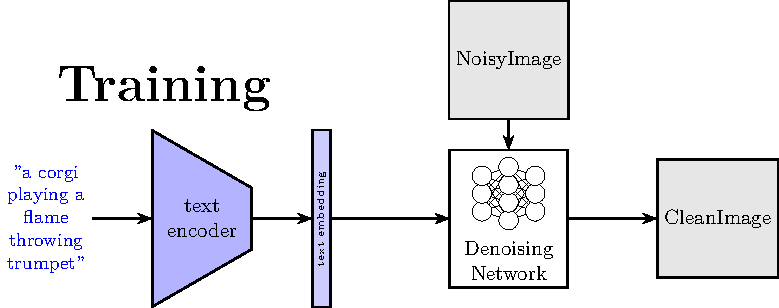
\includegraphics[width=\linewidth]{\toplevelprefix/chapters/chapter6/figs/tti-train.pdf}
    \caption{}
  \end{subfigure}
  \hfill
  \begin{subfigure}{0.47\textwidth}
    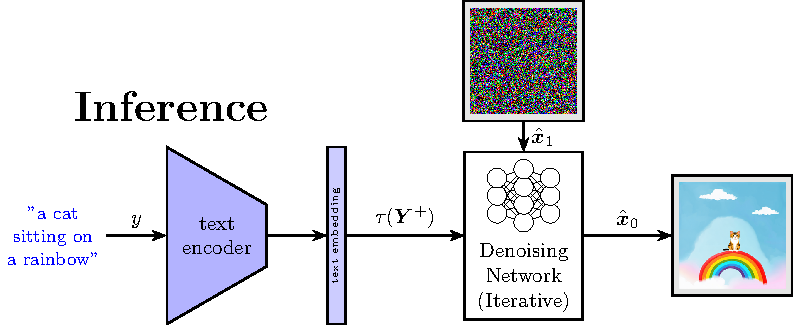
\includegraphics[width=\linewidth]{\toplevelprefix/chapters/chapter6/figs/tti-inf.pdf}
    \caption{}
  \end{subfigure}

  \caption{O schemă de nivel înalt a antrenării și aplicării unui model generativ
  text-la-imagine, prin generare condiționată cu un prompt text. \textbf{Stânga:}
  Pentru a antrena un model text-la-imagine, se folosește un set mare de date de imagini pereche cu
  legende text corespunzătoare. Un codificator este folosit pentru a mapa legendele la
  secvențe de vectori, care sunt folosite ca semnale de condiționare pentru un denoiser
  condiționat, antrenat așa cum este descris în \Cref{sub:cfg}. Codificatorul de text poate fi
  pre-antrenat și înghețat, sau antrenat în comun cu denoiser-ul. \textbf{Dreapta:}
  Când se aplică un model antrenat, un prompt text dorit este folosit ca condiționare,
  apoi se efectuează eșantionarea cu modelul antrenat, ca în
  \Cref{alg:iterative_denoising_conditional_CFG} (\textit{mutatis mutandis} pentru
  utilizare cu un prompt text codat). Pentru detalii complete ale procesului de codare
  a textului într-o secvență de vectori, vezi \Cref{sec:clm_text}.}
  \label{fig:text-to-image}
\end{figure}

Stable Diffusion urmează metodologia de generare condiționată pe care o conturăm în
\Cref{sub:cfg}, cu două modificări cheie: (i) Semnalul de condiționare este un
prompt text tokenizat $\vY$, mai degrabă decât o etichetă de clasă; (ii) Denoising-ul imaginii este
efectuat în spațiul ``latent'' mai degrabă decât pe pixeli bruti, folosind o pereche specializată,
pre-antrenată de autocodor variațional $f : \bR^{D_{\mathrm{img}}} \to
\bR^{d_{\mathrm{img}}}$, $g : \bR^{d_{\mathrm{img}}} \to
\bR^{D_{\mathrm{img}}}$ (vezi \Cref{sec:vae}), unde $f$
este codificatorul și $g$ este decodificatorul. Dezvoltarea ulterioară a modelului a arătat că
punctul (ii) este o problemă de eficiență, mai degrabă decât una conceptuală de bază, așa că nu ne vom
concentra pe ea, altfel decât să menționăm că duce pur și simplu la următoarele
modificări simple ale conductei text-la-imagine schițate în
\Cref{fig:text-to-image}: 
\begin{enumerate}
  \item \textbf{La momentul antrenării},
    codificatorul $f : \vx \mapsto \vz$ este folosit pentru a genera țintele de denoising, și
    tot denoising-ul este efectuat pe reprezentările codate $\vz_t \in
    \bR^{d_{\mathrm{img}}}$;
  \item \textbf{La momentul generării}, eșantionarea este efectuată pe
    reprezentările $\hat{\vz}_t$, și
    imaginea finală este generată prin aplicarea decodificatorului $g(\hat{\vz}_0)$.
\end{enumerate}
În contrast, problema (i) este esențială, iar abordarea propusă pentru a o aborda
reprezintă una dintre inovațiile metodologice durabile ale
\textcite{rombach2022high}.
În contextul cadrului de denoising condiționat iterativ pe care l-am
dezvoltat în \Cref{sub:cfg}, aceasta privește parametrizarea denoiser-elor
$\bar{\vz}_{\theta}(t, \vz_t, \vY^+)$.\footnote{În setarea condiționării pe text,
eticheta `augmentată' $\vY^+$, care este fie promptul text codat,
fie $\varnothing$, denotând denoising necondiționat, este adesea implementată
prin maparea $\varnothing$ la șirul gol ``'', apoi codarea acestui prompt
text cu tokenizatorul ca de obicei. Aceasta oferă o modalitate simplă și unificată de a trata
denoising-ul condiționat și necondiționat cu condiționare pe text.}
\textcite{rombach2022high} implementează condiționarea pe text în denoiser folosind
un strat cunoscut sub numele de atenție încrucișată, inspirat de arhitectura originală
transformer codificator-decodificator a \textcite{vaswani2017attention}. Atenția încrucișată este
implementată după cum urmează. Notăm $\tau : \bR^{D_{\mathrm{text}} \times N} \to
\bR^{d_{\mathrm{model}} \times N_{\mathrm{text}}}$
o rețea de codare pentru încorporările text (adesea un transformer
cauzal---vezi \Cref{sec:clm_text}), și notăm $\psi : \bR^{d_{\mathrm{img}}}
\to \bR^{d_{\mathrm{model}} \times N_{\mathrm{img}}}$ maparea corespunzătoare uneia dintre
reprezentările intermediare în denoiser.\footnote{În practică,
denoiser-ele condiționate pe text adaugă straturi de atenție încrucișată la intervale regulate
în cadrul trecerii directe a denoiser-ului, deci $\psi$ ar trebui văzut ca
dependent de strat, în contrast cu $\tau$. Vezi \textcite{rombach2022high} pentru
detalii.} Aici, $N_{\mathrm{text}}$ este lungimea maximă a promptului text tokenizat,
și $N_{\mathrm{img}}$ corespunde aproximativ numărului de canale de imagine
(dependent de strat) în reprezentare, care este fix dacă rezoluția imaginii de intrare este fixă. Atenția încrucișată (cu $K$ capete, și fără bias) este definită ca
    \begin{equation}
      \mathrm{MHCA}(\vz_t, \vY^+) \label{eq:mhca}
        = \vU_{\out}\mat{\SA([\vU_{\query}^{1}]^{\top}\psi(\vz_t),
        [\vU_{\attnkey}^{1}]^{\top}\tau(\vY^+), [\vU_{\val}^{1}]^{\top}\tau(\vY^+)) \\ \vdots \\
        \SA([\vU_{\query}^{K}]^{\top}\psi(\vz_t),
        [\vU_{\attnkey}^{K}]^{\top}\tau(\vY^+),
        [\vU_{\val}^{K}]^{\top}\tau(\vY^+))}, %
    \end{equation}
unde $\mathrm{SA}$ denotă operația omniprezentă de auto-atenție
în transformer (pe care o reamintim în detaliu în \Cref{ch:applications}: vezi
\Cref{eq:mhsa,eq:self_attention}), și $\vU_{*}^{k} \in \bR^{d_{\mathrm{model}}\times
d_{\mathrm{attn}} }$ pentru $* \in \set{\mathrm{qry}, \mathrm{key}, \mathrm{val}}$
(precum și proiecția de ieșire $\vU_{\mathrm{out}}$) sunt parametrii
învățabili ai stratului.

Observați că, prin definiția operației de auto-atenție, atenția încrucișată
\textit{produce combinații liniare ale încorporărilor text proiectate pe valoare
ponderate de corelațiile dintre caracteristicile imaginii și încorporările text.}
În arhitectura denoiser-ului folosită de \textcite{rombach2022high}, 
blocurile reziduale de auto-atenție din arhitectura denoiser-ului, aplicate la
reprezentarea imaginii la stratul curent și definite analog
celor din \Cref{eq:vit-res-block} pentru transformerul de viziune, sunt urmate de blocuri
reziduale de atenție încrucișată de forma \eqref{eq:mhca}.
O astfel de structură necesită ca codificatorul de text $\tau$ să, într-un anumit sens, împărtășească o anumită
structură în ieșirea sa cu încorporarea caracteristicilor imaginii $\psi$: aceasta poate fi
impusă fie prin pre-antrenare comună adecvată text-imagine (cum ar fi cu CLIP
\cite{Radford2021-ir}), fie prin antrenare comună cu
denoiser-ul însuși (care a fost propusă și demonstrată de
\textcite{rombach2022high}, dar a căzut în dizgrație din cauza costurilor ridicate de date și
antrenare pentru performanță puternică).
Conceptual, acest spațiu comun de încorporare text-imagine și stratul de atenție încrucișată
în sine au o asemănare puternică cu
denoiser-ul condiționat de amestec de Gaussiene pe care l-am derivat în secțiunea
anterioară (reamintiți \eqref{eq:mog-conditional-denoising-unified-operator}), în
cazul special al unei secvențe cu un singur token. Conexiuni mai profunde
pot fi trasate în setarea multi-token urmând cadrul de reducere a ratei
pentru derivarea arhitecturilor de rețea profundă discutat în
\Cref{ch:unrolling}, și manifestat în derivarea arhitecturii CRATE
asemănătoare transformer-ului.

Același design de bază a fost scalat în continuare la dimensiuni și mai mari de model și set de date,
în particular în instanțierile moderne ale Stable Diffusion
\cite{DBLP:conf/icml/EsserKBEMSLLSBP24}, precum și în modele concurente precum
FLUX.1 \cite{Labs2025-fb}, Imagen \cite{Saharia2022-na} și DALL-E \cite{Ramesh2022-nu}. 
Mecanismul de condiționare al atenției încrucișate a devenit de asemenea omniprezent în
alte aplicații, ca în EgoAllo (\Cref{sub:ego-allo}) pentru generarea condiționată de poză și în Michelangelo \cite{zhao2023michelangelo} pentru generarea condiționată de forme 3D bazată pe imagini sau texte.






\section{Inferență Condiționată cu Auto-Consistență a Măsurătorilor}
\label{sec:measurement-self-consistency}
În această ultimă secțiune, considerăm cazul mai extrem, dar de fapt omniprezent, pentru învățarea distribuției în care avem doar un set de eșantioane observate $\Y = \{\y_1,\ldots, \y_N\}$ ale datelor $\x$, dar niciun eșantion direct al lui $\x$! În general, observația $\y \in \mathbb{R}^d$ este de dimensiune mai mică decât $\x \in \mathbb{R}^D$. Pentru a face problema bine definită, presupunem că modelul de observație dintre $\y$ și $\x$ este cunoscut ca aparținând unei anumite familii de modele analitice, notate ca $\y = h(\x, \theta) +\vw$, cu $\theta$ fie cunoscut, fie necunoscut.

Să încercăm mai întâi să înțelegem problema conceptual cu cazul simplu când funcția de măsurare $h$ este cunoscută și $\y = h(\x) + \vw$ observat este informativ despre $\x$. Adică, presupunem că $h$ este surjectivă de la spațiul lui $\x$ la cel al lui $\y$ și suportul distribuției $\y_0 = h(\x_0)$ este de dimensiune redusă. Aceasta necesită de obicei ca dimensiunea \textit{extrinsecă} $d$ a lui $\y$ să fie mai mare decât dimensiunea \textit{intrinsecă} a suportului distribuției lui $\x$. Fără pierderea generalității, putem presupune că există funcții:
\begin{equation}
F(\x) = \boldsymbol{0},\quad     G(\y) = \boldsymbol{0}.
\end{equation}
Observați că aici putem presupune că cunoaștem $G(\y)$ dar nu $F(\x)$. Fie $\mathcal{S}_{\y} \doteq \{\y \mid G(\y) = \boldsymbol{0}\}$ suportul lui $p(\y)$. În general, $h^{-1}(\mathcal{S}_{\y}) = \{\x \mid G(h(\x)) = \boldsymbol{0}\}$ este o supramulțime a $\mathcal{S}_{\x} \doteq \{\x \mid F(\x) = \boldsymbol{0}\}$. Adică, avem $h(\mathcal{S}_{\x}) \subseteq \mathcal{S}_{\y}$.



\subsection{Modele de Măsurare Liniare}
Mai întâi, pentru simplitate, să considerăm că măsurătoarea este o funcție liniară a datelor $\x$ de interes:
\begin{equation}
    \y = \vA\x.
\end{equation}
Aici matricea $\vA \in \mathbb{R}^{m\times n}$ este de rang complet pe rânduri și $m$ este de obicei mai mic decât $n$. Presupunem că $\vA$ este cunoscut deocamdată. Suntem interesați de cum să învățăm distribuția lui $\x$ din astfel de măsurători. Deoarece nu mai avem eșantioane directe ale lui $\x$, ne întrebăm dacă putem încă dezvolta un denoiser pentru $\x$ cu observații $\y$. Să considerăm următorul proces de difuzie:
\begin{equation}
    \y_t = \y_0 + t \vg, \quad \y_0 = \vA(\x_0), 
\end{equation}
unde $\vg \sim \mathcal{N}(\boldsymbol{0}, \vI)$.



Fără pierderea generalității, presupunem că $\vA$ este de rang complet pe rânduri, adică subdeterminat. Să definim procesul corespunzător $\x_t$ ca unul care satisface:
\begin{equation}
\y_t = \vA \x_t.   
\end{equation}

Din procesul de denoising al lui $\y_t$, avem
\begin{equation}
    \y_{t-s} \approx  \y_t + st \nabla \log p_t(\y_t).
\end{equation}
Atunci avem:
\begin{equation}
    \vA\x_{t-s} \approx   \vA\x_t + st \nabla \log p_t(\vA \x_t),
\end{equation}
pentru un $s >0$ mic. Deci $\x_{t-s}$ și $\x_t$ trebuie să satisfacă:
\begin{equation}
    \vA(\x_{t-s} - \x_t) \approx st \nabla \log p_t(\vA\x_t). 
\end{equation}
Dintre toți $\x_{t_s}$ care satisfac constrângerea de mai sus, alegem arbitrar pe cel care minimizează distanța $\|\x_{t-s} - \x_t\|_2^2$. Prin urmare, obținem un proces de ``denoising'' pentru $\x_t$:
\begin{equation}
    \x_{t-s}  \approx \x_t + st\vA^\dagger \nabla \log p_t(\vA\x_t). 
\label{eqn:denoising-projection}
\end{equation}
Observați că acest proces nu eșantionează din distribuția lui $\vx_t$. În particular, există componente ale lui $\vx$ în spațiul nul/nucleul lui $\vA$ care nu pot fi niciodată recuperate din observații. Astfel, mai multe informații sunt necesare pentru a recupera distribuția completă a lui $\vx$, strict vorbind. Dar aceasta recuperează componenta lui $\vx$ care este ortogonală pe spațiul nul al lui $\vA$.





\subsection{Model Vizual 3D din Imagini Calibrate}
În practică, modelul de măsurare este adesea neliniar sau doar parțial cunoscut. O problemă tipică de acest gen este de fapt în spatele modului în care putem învăța un model funcțional al lumii externe din imaginile percepute, să zicem prin ochii noștri, telescoape sau microscoape. În particular, oamenii și animalele sunt capabile să construiască un model al lumii 3D (sau 4D pentru o lume dinamică) printr-o secvență a proiecțiilor sale 2D—o secvență de imagini 2D (sau perechi stereo). Modelul matematic sau geometric al proiecției este în general cunoscut:
\begin{equation}
    \y^i = h(\x, \theta^i) +\vw^{i}, 
\end{equation}
unde $h(\cdot)$ reprezintă o proiecție (perspectivă) a scenei 3D (sau 4D) dintr-o anumită vedere a camerei la timpul $t_i$ la o imagine 2D (sau o pereche stereo) și $\vw$ este un zgomot de măsurare posibil aditiv mic. \Cref{fig:projection-2D} ilustrează această relație concret, în timp ce \Cref{fig:inference_distributed} ilustrează problema model în abstract. O expunere completă a geometriei legate de vederi multiple 2D ale unei scene 3D este dincolo de scopul acestei cărți. Cititorii interesați pot consulta cartea \cite{MaY2003}. Pentru moment, tot ce avem nevoie pentru a continua este că astfel de proiecții sunt bine înțelese și imaginile multiple ale unei scene conțin informații suficiente despre scenă.
\begin{figure}[t]
    \centering
    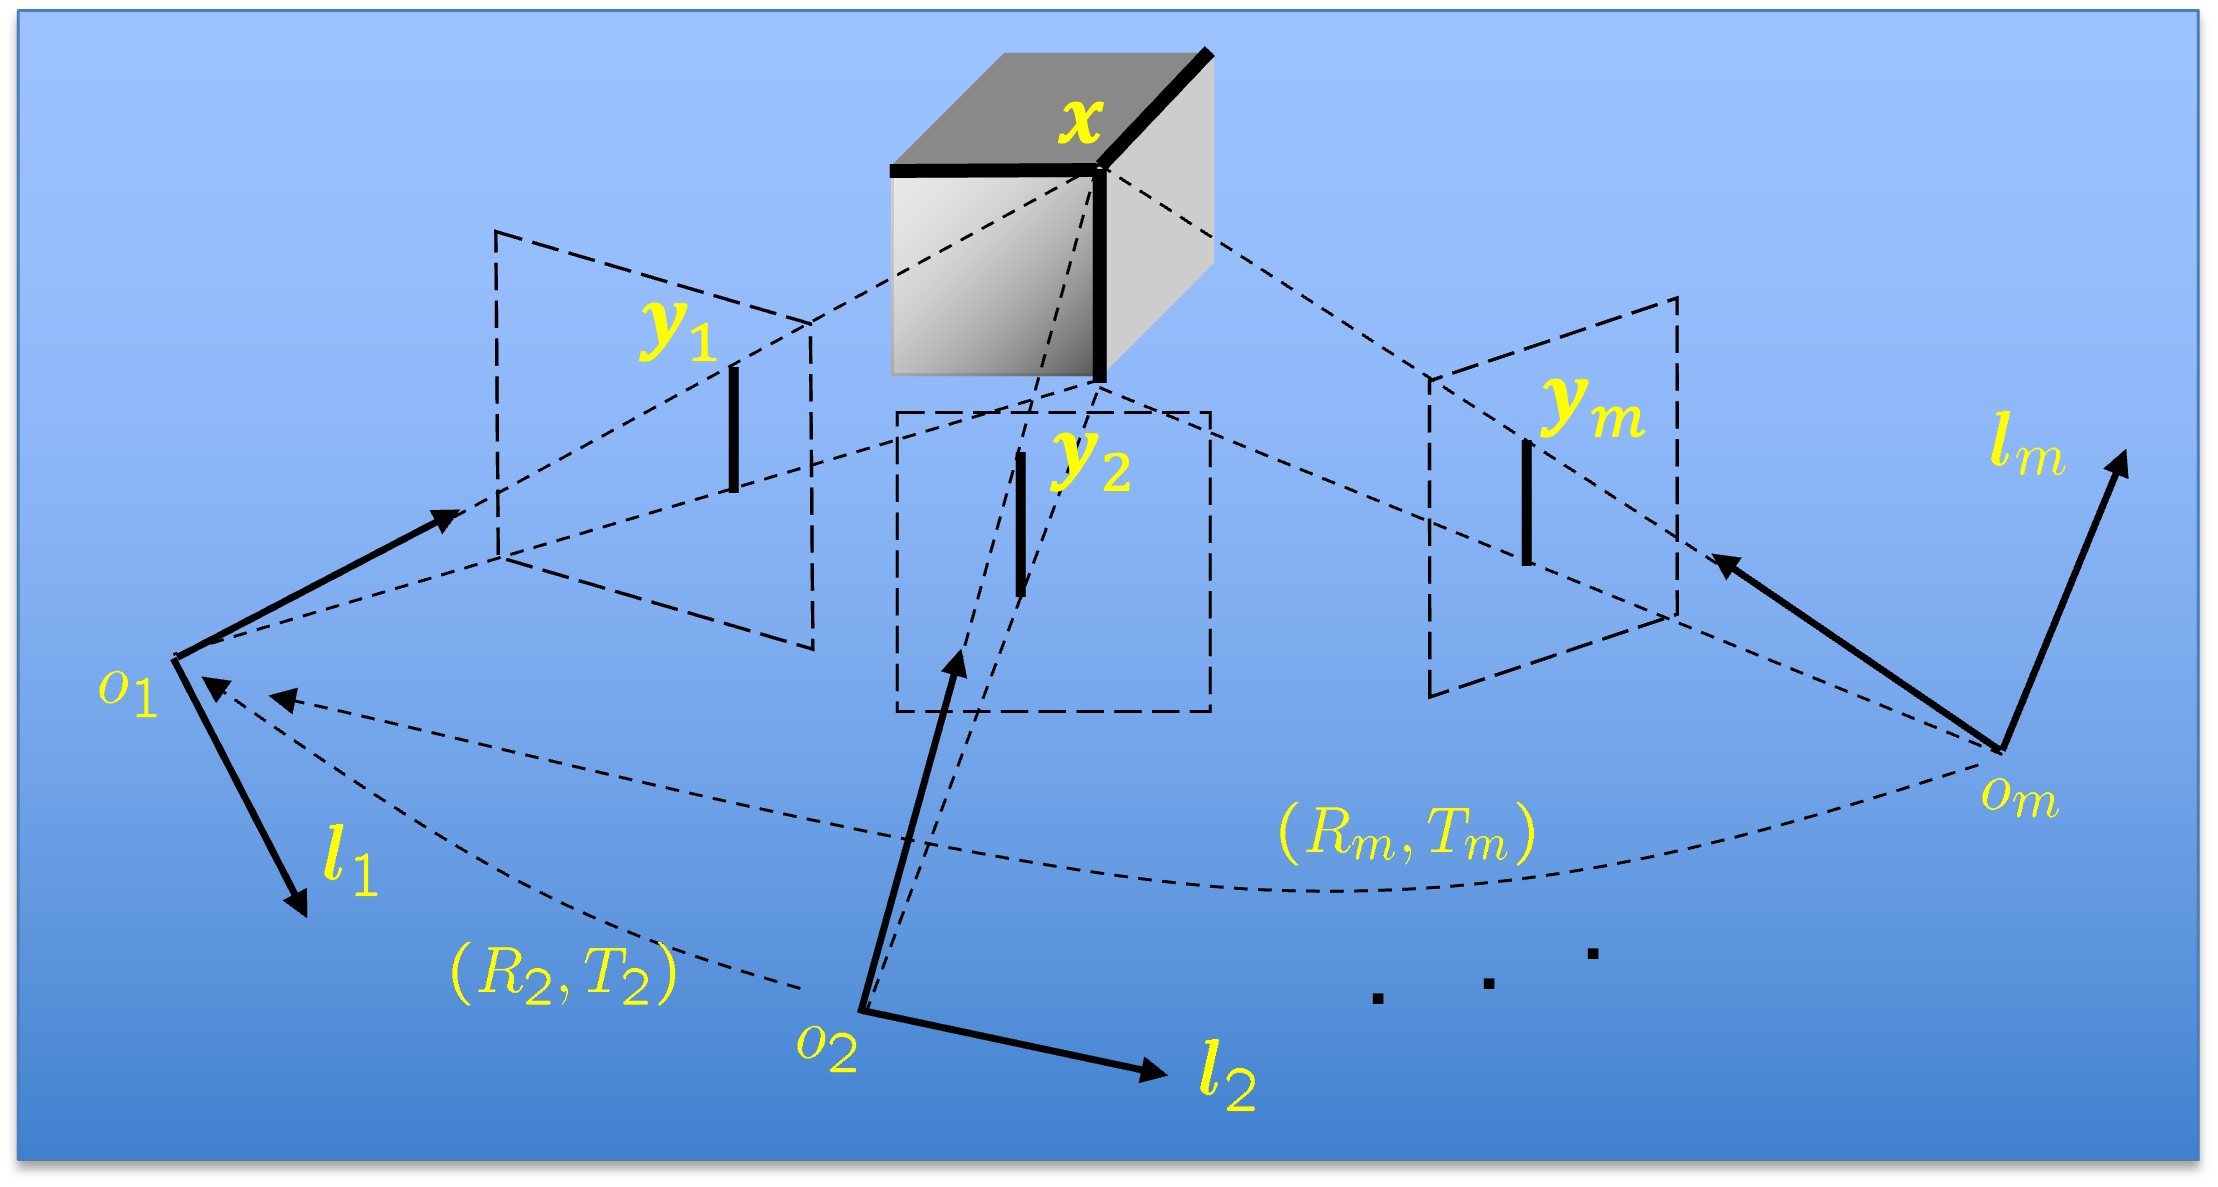
\includegraphics[width=0.7\linewidth]{\toplevelprefix/chapters/chapter6/figs/3D-2D-projection.png}
    \caption{Relația dintre un obiect/scenă 3D și proiecțiile sale 2D. Aici ilustrăm proiecția unui punct $\x$ și a unei linii care intersectează punctul.}
    \label{fig:projection-2D}
\end{figure}

\begin{figure}[t]
  \centering 
  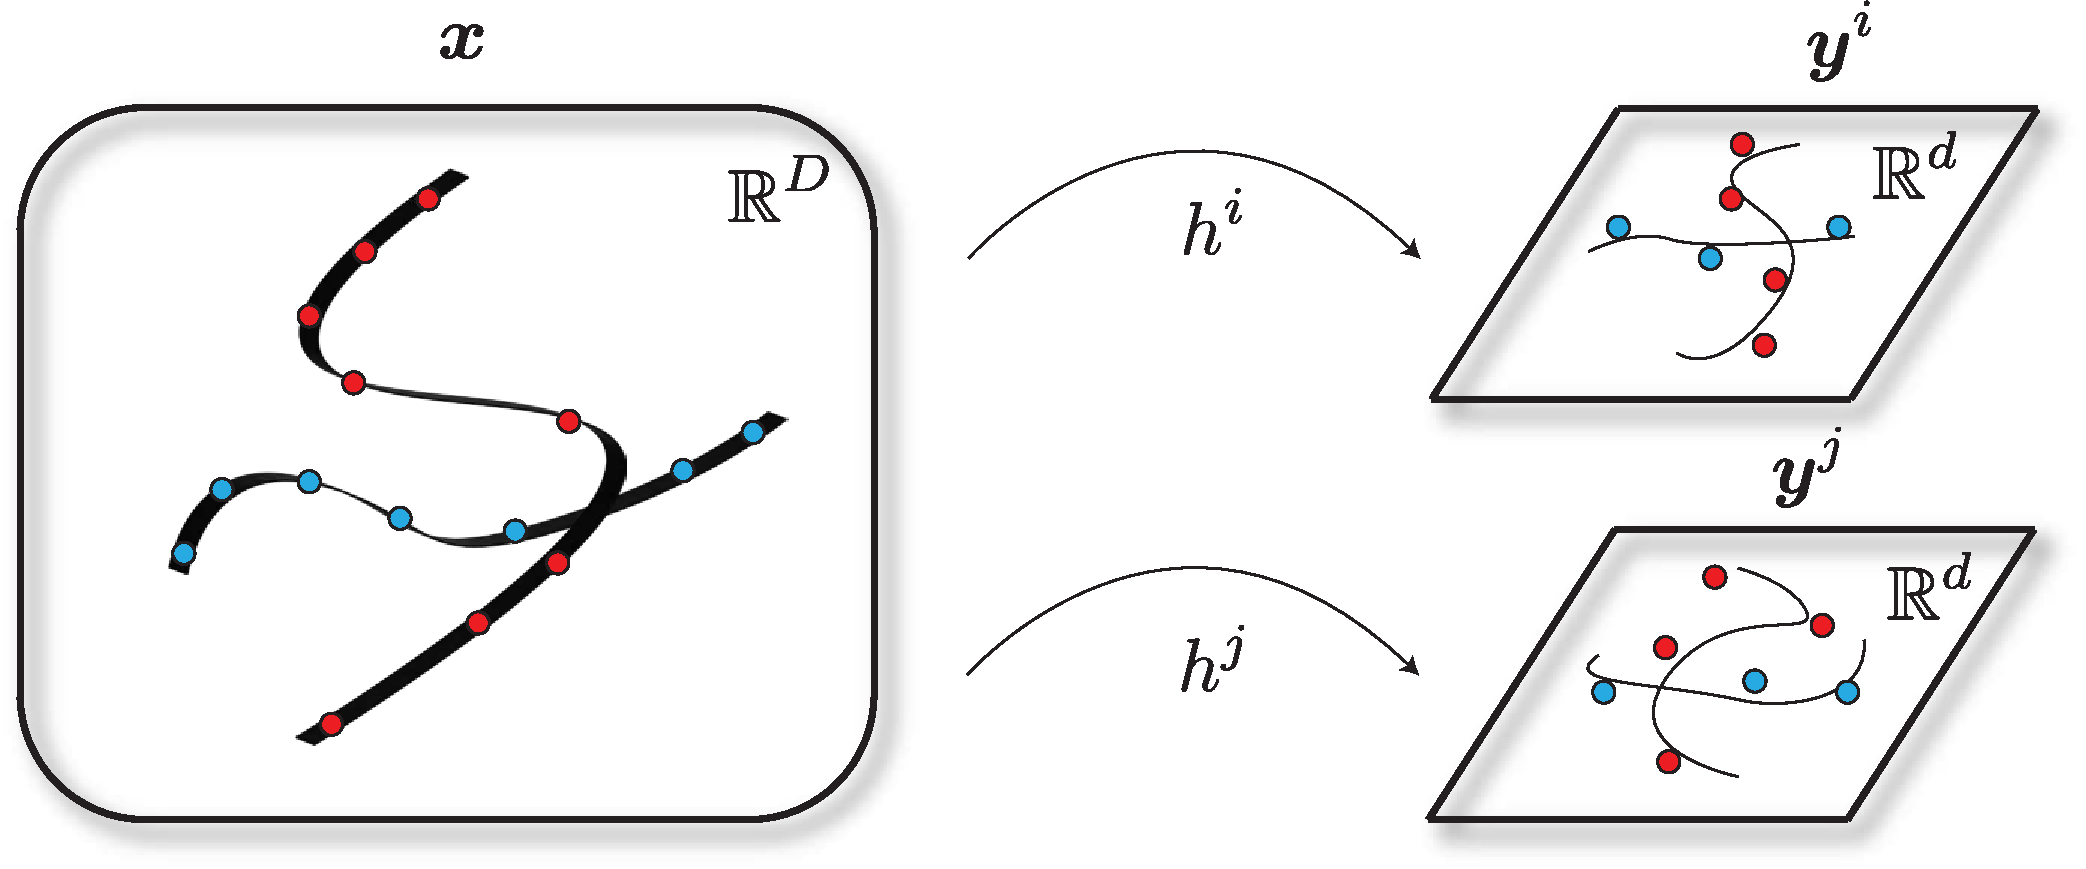
\includegraphics[width=0.7\linewidth]{\toplevelprefix/chapters/chapter6/figs/inference_distributed.pdf}
  \caption{\small \textbf{Inferență cu măsurători distribuite.} Avem o distribuție de dimensiune redusă \(\vx\) (aici, similar cu \Cref{fig:inference_roadmap}, reprezentată ca o uniune de două varietăți \(2\)-dimensionale în \(\R^{3}\)) și un model de măsurare \(\y^{i} = h^{i}(\vx) + \vw^{i}\). Ca înainte, vrem să inferăm diverse proprietăți ale distribuției condiționate a lui \(\vx\) dat \(\vy\), unde \(\vy\) este colecția tuturor măsurătorilor \(\y^{i}\).}
  \label{fig:inference_distributed}
\end{figure}

În general, am dori să învățăm distribuția $p(\x)$ a scenei lumii 3D (sau 4D) $\x$\footnote{Aici, prin abuz de notație, folosim $\x$ pentru a reprezenta fie un punct în 3D, fie o mostră a unui întreg obiect 3D sau o scenă care constă din multe puncte.} din imaginile 2D percepute ale lumii până acum. Funcția principală a unui astfel de model (vizual) al lumii este să ne permită să recunoaștem locuri unde am fost înainte sau să prezicem cum ar arăta scena curentă într-un timp viitor dintr-un nou punct de vedere.

Să examinăm mai întâi cazul special dar important al viziunii stereo. În acest caz, avem două vederi calibrate ale scenei 3D $\x$:
\begin{equation}
    \y^0 = h(\x, \theta^0) +\vw^0, \quad \y^1 = h(\x, \theta^1) +\vw^1, 
\end{equation}
unde parametrii $\theta_0$ și $\theta_1$ pentru pozele vederilor pot fi presupuși a fi cunoscuți. $\y^0$ și $\y^1$ sunt două proiecții 2D ale scenei 3D $\x$. Putem presupune de asemenea că au aceeași distribuție marginală $p(\y)$ și am învățat un model de difuzie și denoisificare pentru aceasta. Adică, cunoaștem denoiser-ul:
\begin{equation}
  \bE[\vy \mid \vy_t=\vnu] =
  \vnu + t^2 \nabla_{\vnu}\log p_t(\vnu). 
 \label{eq:y-posterior-sampling-denoiser}    
\end{equation}
Sau, mai mult, putem presupune că avem un număr suficient de mostre de perechi stereo $(\y^0, \y^1)$ și am învățat de asemenea distribuția comună a perechilor. Prin un mic abuz de notație, folosim de asemenea $\y = h(\x)$ pentru a indica perechea $\y = (\y^0, \y^1)$ și $p(\y)$ ca distribuția de probabilitate învățată a perechii (să zicem prin intermediul unui denoiser ca mai sus).

Întrebarea principală acum este: Cum să învățăm (o reprezentare pentru) distribuția scenei 3D $\x$ din cele două proiecții ale sale cu relații cunoscute?
Oamenii ar putea pune la îndoială rațiunea pentru a face acest lucru: de ce este necesar dacă funcția $h(\cdot)$ este în mare parte inversabilă? Adică, observația $\y$ poate determina în mare parte necunoscuta $\x$, ceea ce este cumva cazul pentru stereo—în general, două imagini (calibrate) conțin informații suficiente despre adâncimea scenei, din punctul de vedere dat. Cu toate acestea, imaginile 2D sunt departe de a fi cea mai compactă reprezentare a scenei 3D, deoarece aceeași scenă poate produce infinit de multe imagini 2D (foarte corelate) sau perechi de imagini. De fapt, o bună reprezentare a unei scene 3D ar trebui să fie invariantă la punctul de vedere. Prin urmare, o reprezentare corectă a distribuției scenelor 3D ar trebui să fie mult mai compactă și structurată decât distribuția imaginilor 2D, a perechilor stereo sau a perechilor imagine-adâncime.

Considerați procesul (invers) de denoisificare pentru difuzie: $\y_t = \y + t\vg $ în \eqref{eq:y-posterior-sampling-denoiser}, unde $\vg$ este Gaussian standard. Din procesul de denoisificare din \eqref{eq:y-posterior-sampling-denoiser}, avem
\begin{equation}
    \y_{t-s} =  \y_t + st \nabla_{\y} \log p_t(\y_t).
\end{equation}
Încercăm să găsim un proces corespunzător de „denoisificare" al lui $\x_t$ astfel încât $\x$ să fie legat de $y$ ca:
\begin{equation}
    \y =  h(\x).
\end{equation}

Atunci avem:
\begin{equation}
    h(\x_{t-s}) \approx  h(\x_t) + st \nabla_{\y} \log p_t(h(\x_t)),
\end{equation}
pentru un $s >0$ mic.
Presupunem că $\x_{t-s} = \x_t + s \vv$ pentru un anumit vector $\vv$ și increment mic $s$. Avem
\begin{equation}
    h(\x_{t-s}) \approx h(\x_t) + \frac{\partial h}{\partial \x}(\vx_{t}) \cdot \vv s \doteq h(\x_t) + \vA(\x_t) \vv s. 
\end{equation}
Prin urmare, avem
\begin{equation}
    \vA(\x_t) \vv = t \nabla_{\y} \log p_t(h(\x_t)).
    \label{eqn:pushforward}
\end{equation}
Geometric, vectorul $\vv$ în domeniul lui $\x$ poate fi văzut ca pullback-ul câmpului vectorial $t \nabla \log p_t(\y)$ sub harta $\y = h(\x)$. În general, ca înainte, putem alege (arbitrar) $\vv$ să fie vectorul cu norma 2 minimă care satisface relația de pullback. Prin urmare, putem exprima $\hat{\x}_{t-s}$ aproximativ ca:
\begin{equation}
    \hat{\x}_{t-s} \approx \x_t + st\vA(\x_t)^\dagger \nabla_{\y} \log p_t(h(\x_t)). 
\label{eqn:pullback-denoise}
\end{equation}


\begin{remark}[Detectare Paralelă și Denoisificare Distribuită.]
{Există ceva foarte interesant despre ecuația de mai sus \eqref{eqn:pullback-denoise}. Pare să sugereze că am putea încerca să învățăm distribuția lui $\x$ printr-un proces care este cuplat cu (multe dintre) observațiile sale (parțiale):
\begin{equation}
\y^i = h^i(\x) +\vw^i, i =1, \ldots, K.
\end{equation} În acest caz, obținem un set de ecuații pe care câmpul vectorial $\vv$ în domeniul lui $\x$ ar trebui să le satisfacă:
\begin{equation}
    \vA^i(\x_t) \vv = t \nabla_{\y^i} \log p_t(h^i(\x_t)),
\label{eqn:federated-pushforward}
\end{equation}
unde $\vA^i(\x_t) = \frac{\partial h^i}{\partial \x}(\vx_t)$. $\vv$ final poate fi ales ca o soluție „centralizată" care satisface toate ecuațiile de mai sus, sau ar putea fi ales ca o versiune „agregată" (stocastic) a tuturor $\vv^i$:
\begin{equation}
    \vv^i = t\vA^i(\x_t)^\dagger \big[\nabla_{\y^i} \log p_t(h^i(\x_t))\big], \quad i = 1, \ldots, K,
\end{equation}
care sunt calculate într-o manieră paralelă și distribuită? O întrebare deschisă aici este exact la ce converge procesul de „denoisificare" astfel definit pentru $\x_t$, chiar și în cazul modelului de măsurare liniară. Când ar converge la o distribuție care are același suport de dimensiune redusă ca $\x_0$ original, pe măsură ce $\y_t$ converge la $\y = h(\x_0)$? }
\end{remark}



\paragraph{Model Vizual al Lumii din Secvențe de Imagini Necalibrate}

În derivarea de mai sus, am presupus că modelul de măsurare $h(\cdot)$ este complet cunoscut. În cazul viziunii stereo, acest lucru este destul de rezonabil, deoarece poza relativă (și calibrarea) celor două vederi ale camerei (sau a celor doi ochi\footnote{Poza relativă a celor doi ochi ai noștri este bine cunoscută creierului nostru.}) este de obicei cunoscută în avans. Prin urmare, prin perechile de imagini stereo, în principiu ar trebui să putem învăța distribuția scenelor 3D, cel puțin distribuția ego-centrică a scenelor 3D. Cu toate acestea, structurile de dimensiune redusă ale așa-numitei distribuții învățate conțin variații cauzate de schimbarea punctelor de vedere. Adică, aspectul imaginilor stereo variază când ne schimbăm punctele de vedere în raport cu aceeași scenă 3D. Pentru multe sarcini practice de viziune (cum ar fi localizarea și navigarea), este important să putem decupla această variație a punctelor de vedere de o reprezentare invariantă a (distribuției) scenelor 3D.

\begin{remark}Rețineți că obiectivul de mai sus se aliniază bine cu Programul Erlangen al lui Klein pentru geometria modernă, care este de a studia invarianții unei varietăți sub un grup de transformări. Aici, putem vedea varietatea de interes ca distribuția reprezentărilor ego-centrice ale scenelor 3D. Am învățat că admite un grup de mișcare rigidă tridimensională care acționează asupra ei. Este remarcabil că creierul nostru a învățat să decupleze eficient astfel de transformări de lumea 3D observată.
\end{remark}


Observați că am studiat învățarea reprezentărilor care sunt invariante la translație și rotație într-o setare limitată în Capitolul \ref{ch:representation}. Știm că operatorii de compresie asociați iau forma necesară de convoluții (multi-canal), conducând astfel la rețelele neuronale convoluționale (profunde). Cu toate acestea, operatorii care sunt asociați cu compresia sau denoisificarea care sunt invariante la grupuri de transformare mai generale rămân evazivi de caracterizat \cite{cohen2016group}.
Pentru problema Viziunii 3D în setarea sa cea mai generală, știm că schimbarea punctelor noastre de vedere poate fi bine modelată ca o mișcare de corp rigid. Cu toate acestea, mișcarea relativă exactă a ochilor noștri între diferite puncte de vedere nu este de obicei cunoscută. Mai general, ar putea exista și obiecte (de exemplu, mașini, oameni, mâini) care se mișcă în scenă și în mod normal nu știm mișcarea lor. Cum putem generaliza problema învățării distribuției scenelor 3D cu perechi stereo calibrate la astfel de setări mai generale? Mai precis, vrem să învățăm o reprezentare compactă $\x$ a scenelor 3D care este invariantă la mișcările camerei/ochiului. Odată ce o astfel de reprezentare este învățată, am putea eșantiona și genera o scenă 3D și reda imagini sau perechi stereo din poze arbitrare.


În acest scop, rețineți că putem modela o secvență de perechi stereo ca:
\begin{equation}
    \y^k = h(\x^k, \theta^k), \quad k=1, \ldots, K,
\end{equation}
unde $h(\cdot)$ reprezintă harta de proiecție de la 3D la 2D. $\theta^k$ denotă parametrii de mișcare de corp rigid ai vederii $k$, în raport cu un anumit cadru canonic în lume. $\x^k$ reprezintă scena 3D la timpul $k$. Dacă scena este statică, $\x^k$ ar trebui să fie toate la fel $\x^k = \x$. Pentru a simplifica notația, putem denota setul de $k$ ecuații ca una:
\begin{equation}
    \Y = H(\x,\Theta). 
\end{equation}
Putem presupune că ni se dau multe mostre de astfel de secvențe de imagini stereo $\{\Y_i\}$. Problema este cum să recuperăm secvența de mișcare asociată $\{\Theta_i\}$ și să învățăm distribuția scenei $\x$ (care este invariantă la mișcare). După cunoștințele noastre, aceasta rămâne o problemă deschisă provocatoare, probabil ca frontiera finală pentru problema Viziunii 3D.




\section{Rezumat și Note}
\paragraph{Potrivirea măsurătorilor fără mostre curate.} În dezvoltarea noastră a
eșantionării condiționate, am considerat potrivirea măsurătorilor sub un model
de observare \eqref{eq:measurement-matching-observation}, unde presupunem că avem
date împerecheate $(\vx, \vy)$—adică, adevărul de bază pentru fiecare observație $\vy$.
În multe probleme inverse relevante practic, acesta nu este cazul: unul dintre
cele mai fundamentale exemple este în contextul detectării comprimate, pe care am
reamintit-o în \Cref{ch:classic}, unde trebuie să reconstruim $\vx$ din $\vy$
folosind cunoștințe anterioare despre $\vx$ (adică, raritate).
În setarea denoisificare-difuzie, avem acces la o prioritate implicită pentru
$\vx$ prin intermediul denoiser-ilor învățați $\bar{\vx}_{\theta}(t, \vxi)$. Putem totuși efectua
eșantionare condiționată fără acces la mostre de adevăr de bază $\vx$?

Pentru intuiție cu privire la de ce acest lucru ar putea fi posibil, ne amintim un exemplu clasic
din statistică cunoscut sub numele de estimatorul de risc imparțial al lui Stein (SURE).
Sub un model de observare $\vx_t = \vx + t \vg$ cu $\vg \sim \cN(\Zero,
\vI)$ și $t>0$, se dovedește că pentru orice $f : \bR^D \to \bR^D$ slab diferențiabil,
\begin{equation}\label{eq:sure-risk}
  \bE_{\vg}\left[
    \norm*{\vx - f(\vx + t \vg)}_2^2
    \right]
  =
  \bE_{\vg}\left[
    \norm*{\vx+t\vg - f(\vx + t \vg)}_2^2
    + 2t^2 \nabla \cdot f(\vx + t\vg)
    \right]
  - t^2 D,
\end{equation}
unde $\nabla \cdot$ denotă operatorul de divergență:
\begin{equation*}
	\nabla \cdot f = \sum_{i=1}^D \partial_i f_i.
\end{equation*}
Partea dependentă de $\vx$ din RHS din \Cref{eq:sure-risk} se numește estimatorul
de risc imparțial al lui Stein (SURE). Dacă luăm așteptări peste $\vx$ în \Cref{eq:sure-risk},
rețineți că RHS poate fi scris ca o așteptare în raport cu $\vx_t$---în
special, eroarea pătratică medie a \textit{oricărui denoiser $f$} poate fi estimată
\textit{doar din mostre zgomotoase}!
Acest fapt remarcabil, în forme rafinate, constituie baza pentru multe tehnici
practice pentru efectuarea restaurării imaginii, denoisificare-difuzie, etc.\ folosind
doar date zgomotoase: exemple notabile includ paradigma „noise2noise"
\cite{pmlr-v80-lehtinen18a}
și Ambient Diffusion \cite{daras2023ambient}.

Ca o paranteză amuzantă, subliniem că \Cref{eq:sure-risk} conduce la o dovadă
alternativă a formulei lui Tweedie (\Cref{thm:tweedie}). La un nivel înalt, se iau
așteptări peste $\vx$ și se exprimă partea principală a RHS din
\Cref{eq:sure-risk} echivalent, prin integrare prin părți, ca
\begin{equation}
  \bE_{\vx_t}\left[
    \norm*{\vx_t - f(\vx_t)}_2^2
    + 2t^2 \nabla \cdot f(\vx_t)
    \right]
  =
  \bE_{\vx_t}\left[
    \norm*{\vx_t - f(\vx_t)}_2^2
    \right]
  - 2t^2 \int
  \ip*{\nabla p_{\vx_t}(\vxi)}{f(\vxi)}
  \odif \vxi.
\end{equation}
Aceasta este o funcție pătratică a lui $f$, și luarea formală a derivatelor dă
că $f$ optim satisface formula lui Tweedie (\Cref{thm:tweedie}). Acest
argument poate fi făcut riguros folosind idei de bază din calculul variațiilor.


\paragraph{Corecții la aproximarea Diffusion Posterior Sampling (DPS).}
În \Cref{example:denoising-conditional-gaussian} și în special în
\Cref{fig:conditional_sampling_computational_gaussian}, am subliniat
o limitare a aproximării DPS
\Cref{eq:conditional-posterior-measurementmatching-gaussian-case-dps-approx} la
niveluri mici de zgomot de măsurare.
Această limitare este bine înțeleasă, și o abordare principială pentru ameliorarea ei
a fost propusă de Rozet et al.\ \cite{rozet2024learning}.
Abordarea implică încorporarea unei estimări suplimentare pentru varianța
posteriorului zgomotos $p_{\vx \mid \vx_t}$ la
\Cref{eq:conditional-posterior-measurementmatching-gaussian-case-dps-approx}---ne
referim la lucrare pentru detalii.
Estimările naturale pentru varianța posterioară sunt ușor mai puțin scalabile decât DPS
în sine din cauza necesității de a inversa o transformare afină a Jacobianului
denoiser-ului posterior $\bE[\vx \mid \vx_t=\vxi]$ (o matrice mare). Acest lucru se face
relativ eficient de Rozet et al.\ \cite{rozet2024learning} folosind diferențiere automată și o
aproximare pentru inversă bazată pe gradienți conjugați. Se pare că ar trebui
să fie posibil să se îmbunătățească în continuare această abordare (să zicem, folosind idei
clasice din optimizarea de ordinul doi).


\paragraph{Mai multe despre potrivirea măsurătorilor și modelele de difuzie pentru probleme
inverse.}

Modelele de difuzie au devenit un instrument extrem de popular pentru rezolvarea problemelor
inverse care apar în aplicațiile științifice. Multe mai multe metode dincolo de simplul
algoritm DPS pe care l-am prezentat în \Cref{alg:iterative_denoising_conditional_DPS} au fost
dezvoltate și continuă să fie dezvoltate, deoarece zona evoluează rapid.
Clasele populare și performante de abordări dincolo de DPS, pe care le-am prezentat
din cauza generalității sale, includ abordări de împărțire a variabilelor precum DAPS
\cite{Zhang2024-ha},
care permit ca constrângerile specifice de măsurare să fie impuse mult mai
puternic decât în DPS, și abordări exacte care pot evita utilizarea
aproximărilor ca în DPS, cum ar fi TDS \cite{wu2023practical}.
Pentru mai multe despre această zonă, recomandăm \cite{zheng2025inversebench}, care
funcționează simultan ca un sondaj și un benchmark al mai multor metode populare
pe seturi de date specifice de probleme inverse științifice.

\section{Exerciții și Extensii}


\begin{exercise}[Corecția Varianței Posterioare la DPS]

  \begin{enumerate}
    \item Folosind codul furnizat în GitHub-ul cărții pentru implementarea
      \Cref{fig:conditional_sampling_computational_gaussian}, implementați
      corecția varianței posterioare propusă de \textcite{rozet2024learning}.
    \item Verificați că ameliorează problema colapsului posterior la varianță
      scăzută a zgomotului observată în
      \Cref{fig:conditional_sampling_computational_gaussian}.
    \item Discutați orice probleme de corectitudine a eșantionării care sunt reținute sau
      introduse de metoda corectată, precum și eficiența sa, relativ la
      diffusion posterior sampling (DPS).
  \end{enumerate}

\end{exercise}

\begin{exercise}[Eșantionare Condiționată pe MNIST]
  \begin{enumerate}
    \item Antrenați un clasificator simplu pentru setul de date MNIST, folosind o arhitectură
      la alegerea dumneavoastră. În plus, antrenați un denoiser potrivit pentru utilizare în
      eșantionarea condiționată (\Cref{alg:iterative_denoising_conditional_CFG},
      deoarece acest denoiser poate fi folosit și pentru denoisificare necondiționată).
    \item Integrați clasificatorul într-un eșantionator condiționat bazat pe
      ghidare prin clasificator, așa cum este descris în prima parte a \Cref{sub:cfg}.
      Evaluați mostrele rezultate în termeni de fidelitate față de
      clasa de condiționare (vizual; în termeni de cel mai apropiat vecin; în termeni de
      ieșirea clasificatorului).
    \item Integrați clasificatorul într-un eșantionator condiționat bazat pe
      ghidare fără clasificator, așa cum este descris în \Cref{sub:cfg} și
      \Cref{alg:iterative_denoising_conditional_CFG}. Efectuați aceeași
      evaluare ca în pasul anterior și comparați rezultatele.
    \item Repetați experimentul pe setul de date CIFAR-10.
  \end{enumerate}


\end{exercise}


\end{document}

